\documentclass[a4paper,11pt,pdf]{pacmanreport}

%%=== Aditional packages
\usepackage{bm}
\usepackage{mhchem} % Package for chemical equation typesetting
\usepackage{siunitx} % Provides the \SI{}{} command for typesetting SI units
\usepackage{epstopdf}
\usepackage{amsmath}
\usepackage{amssymb}
\usepackage{colortbl}
\usepackage{gensymb}
\usepackage{algorithm}
\usepackage{algorithmic}

% The following is used to make packages hyperref and cite work together
\makeatletter
\let\NAT@parse\undefined
\makeatother
\usepackage[bookmarks=true,hyperfootnotes=true,colorlinks=true,linkcolor=blue,anchorcolor=blue,citecolor=blue,urlcolor=blue,filecolor=blue]{hyperref}

%%=== Local definitions
% Table float box with bottom caption, box width adjusted to content
\DeclareMathOperator{\rad}{rad}

\graphicspath{{images/}{../shared_images/}}

%% ================================
%% PROJECT INFO

\project{}
\projectid{FP7-IST-60918}
\projectstart{1 March 2013}
\duration{36}

%% ================================
%% DELIVERABLE INFO

\title{Control algorithms for haptic object exploration}
\deliverableid{DR 3.1}
\author{C. Rosales, M. Bonilla, G. Santaera, E. Luberto, M. Gabiccini, Jeremy L. Wyatt}
\address{Centro di Ricerca ``E. Piaggio'', Universit\`{a} di Pisa}
\email{carlos.rosales@for.unipi.it}
\headertitle{Haptic exploration}
\headerauthor{C. Rosales, G. Santaera, E. Luberto, M. Gabiccini, J. L. Wyatt}

\duedate{2015-02-28}
\submissiondate{2014-02-28}
\leadpartner{Universit\`{a} di Pisa}
\revision{draft}
\disseminationlevel{PU}

%% UNCOMMENT: to get the logo; if you've copied this file to a directory yearX/wpY/ then this should work
\reportlogo{pacmanlogo.png}

\begin{document}

\maketitle

\begin{abstract}
\noindent This report describes activities related to the development of haptic object exploration methodologies. Object shape refinement and friction coefficient estimation require low-level controllers that allow contour tracing interaction as well as a sophisticated sensorization of the exploratory probe. This report presents the efforts on providing controllers to perform sliding and rolling of a fingertip over a surface, integrating controller strategies with vision, implementing a robust testbed to simulate results, and last but not least, specifying the designs on the sensorization of the Pisa/IIT SoftHand.
\end{abstract}

\vspace{.2em}
\hrule

\footnotesize

\tableofcontents

\normalsize

\newpage

\section*{Executive Summary}
This report describes the activities within the PaCMan consortium to define methodologies for \emph{haptic object exploration}. The material included in this report shows the results of Task 3.1 (M 1-24). Aside, progress of Task 3.2 (M 18-36) along with the envision of a promising approach to tackle the problem of information gathering for unknown objects. Developments of Task 3.3 (M 1-30) and its relation with WP4 is also reported.

\section*{Role of haptic object exploration in PaCMan}

This deliverable reports the research done on finding a methodology to explore objects by touch and vision, and gather their haptic properties such as the static and dynamic friction coefficient.
%To this end, \emph{control algorithms} and \emph{innovative sensors} are developed.

\section*{Contribution to the PaCMan scenario}

The multi-modal object representation to be reported in WP2 requires information about the shape and haptic properties of an object.
The active acquisition of such information is essential to build the representation of a particular object. The exploratory strategies which combine low-level control algorithms developed by the UNIPI team, high-level decision making strategies to be completed by UoB team, together with a sensorized adaptive hand as proposed from the UNIPI team, make this possible.

Additionally, the developed algorithms make no assumption on how the gathered information is encoded. This provides a flexible testbed to contrast the representation coming from WP2 with approaches external to the project.

\newpage

\section{Tasks, objectives, results}

\subsection{Planned work}

This report must show the results of Task 3.1. Particularly, it should describe reactive control strategies for haptic exploration of an object by a robotic hand, consisting of contour tracing of the object surface and finger rolling over the object surface, as well as strategies for extracting higher-order geometric features and frictional properties. 

% In Task 3.3 we planned to implement the active gaze model we presented in year 1 in the robot platform. This was intended to be used in the demonstration 5.2. The hypothesis to be tested is whether a reward based framework for active gaze control for grasping under positional uncertainty can be extended to work on real objects. The initial assumption was that the active gaze control model would work with a prior model of the object shape. The overall goal was to show that active gaze can improve the reliability of grasping and manipulation.

\subsection{Actual work performed}

\subsubsection{Task 3.1}

We can proudly say that Task 3.1 has been accomplished. The results from this task crystallized in~\cite{Rosales2014Active} which is appended in Sec.~\ref{sec:slidingPointClouds}. Details on how the planned activities were followed are described in MS 4.2.

In previous approaches, in general, the friction coefficient is neglected during acquisition when being in contact with the object. For instance,~\cite{Ilonen2013Fusing} fuses the two sources of information, visual and tactile, by applying symmetry constraints to reconstruct the complete object shape, and~\cite{Chalon2013Online} uses the contact points to improve the object pose within the hand, initially obtained by vision. Nonetheless, other object properties apart from the shape are hardly explored, perhaps due to the fact that one needs specific sensory systems to measure them and a proper representation to process the information. In our work, the hardware setup resembles that of~\cite{Bajcsy1984What}, but instead of using tactile arrays at the tip of the exploratory probe, we use an intrinsic tactile sensor based on~\cite{Serio2014Tactile} due to of its capability to retrieve the contact point and force~\cite{Bicchi1993Contact}, which is necessary to our approach. Thus, in the paper we propose a way to estimate the friction coefficient from an object that has been previously detected from vision. The visual information is encoded using a Gaussian Process which then is exploited to generate trajectories over the object surface, which then is explored by means of sliding controllers implemented within the project (see MS 4.2 and Sec~\ref{sec:slidingPointClouds}). The friction coefficient is also encoded using a Gaussian process using both visual and tactile shape measurements. The latter provides a common probabilistic framework for both representations, however, we plan to replace such codification with the output of WP 2 during year 3.

% To be prepared by: Carlos
% Learning the haptic characteristics of objects by exploration in-hand
% %%% Learning the haptic characteristics of objects by exploration in-hand

\subsubsection{Learning the haptic characteristics of objects by exploration in-hand}
\label{sec:ControlAlgorithms}

This report used a fixture device as the supporting hand, and a 7 DOF robot as the exploratory finger. It is worth mentioning that a strategy for concurrent stable object grasping was demonstrated in DR5.1, and assumed to be given for the work presented here, and here we refer to the haptic exploration strategies only.

\paragraph{(a) Definition of control strategies for concurrent stable object grasping and object surface tracing for haptic exploration}

An Arimoto-PD regulator provides the required torques to track a reference position. The position control law is
\begin{equation}
    \bm{\tau_p} = G(\bm{q}) + K_{P_p} \left(\bm{\dot{q}_d}\Delta T\right) + K_{D_p}\bm{\dot{q}},
\end{equation}
where $G(\bm{q})$ is the gravity load vector, $\bm{{q}}$  is the generalized joint variables, $\bm{\dot{q}}$ is the measured rate of joints variables, $\Delta T$ the control period, and $K_{P_p}$,$K_{D_p}$ two positive definite matrices.

% \begin{figure}
% \begin{center}
% 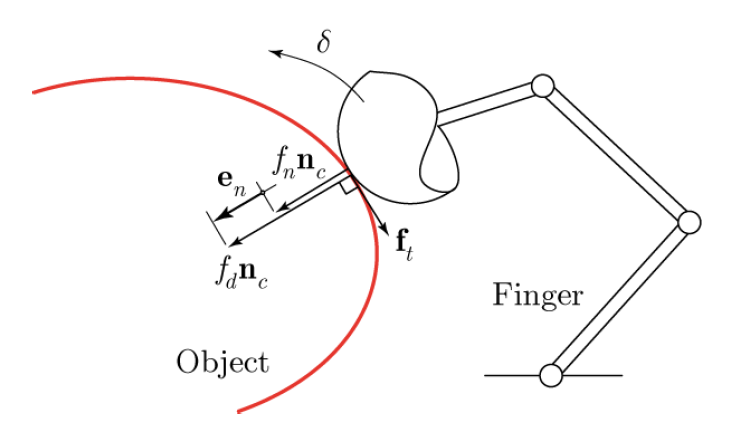
\includegraphics[width=0.65\textwidth]{finger_surface.png}
% \caption{Finger in contact with the unknown surface}
% \label{fig:finger_surface}
% \end{center}
% \end{figure}

A PID force controller is required to ensure contact during motion. The force control law is
\begin{equation}
    \bm{\tau_f} = f_dJ^T\bm{n_c} + K_{P_f}\bm{\tau_{e_n}} + K_{I_f}\int\bm{\tau_{e_n}}dt + K_{D_f}\dot{\bm{\tau}}_{e_n},
\end{equation}
where $J$ is the robot Jacobian matrix, $\bm{e_n} = (f_d - f_n)\bm{n_c}$ is the normal force error, $\bm{\tau_{e_n}} = J^T(\bm{q})\bm{e_n}$ is the normal force error in terms of joints torques, $\bm{v_d}$ the desired twist of the end effector, and $\bm{\dot{q}_d} = J^+\bm{v_d}$ the desired rate of angular joints.

Note that the position and force are to be controlled on the tangent plane and in the direction normal to it, hence due to their orthogonality, we can decouple the actions and sum up the contribution of each controller to form a hybrid force/position controller.

The strategy to slide a finger over a surface consist in assigning a reference velocity on the tangent plane at the contact point, of the same contact point. Let $C$ be the contact point and $\left\lbrace T \right\rbrace$ the frame with $C$ as origin, such that the $y$-$z$ directions form the local tangent plane and the $x$ direction is normal to the fingertip surface and pointing outwards, the desired twist of the fingertip with respect to $C$ written in $\left\lbrace T \right\rbrace$ is
\begin{equation}
    \bm{^Tv_C}=\left(
    \begin{matrix}
        0\\
        v_{dy}\\
        v_{dz}\\
        0\\
        0\\
        0
    \end{matrix}\right),
\end{equation}
where $v_{dy}$ and $v_{dz}$ are scalar components of the desired velocity in the local tangent plane, and $\sqrt{{v_{dy}}^2+{v_{dx}}^2}$ the norm of the assigned velocity. This is called the sliding primitive.

The desired twist of the fingertip center point, $P$, written in the end-effector frame $\left\lbrace E \right\rbrace$ is
\begin{equation}
\bm{^Ev_P}=\left(
    \begin{array}{cc}
       \bm{I}_{3x3} & ^E\hat{\bm{c}} \\
       \bm{0}_{3x3} & \bm{I}_{3x3}
    \end{array}
    \right)
    \left(
    \begin{array}{cc}
        R_{ET} & \bm{0}_{3x3} \\
        \bm{0}_{3x3} & R_{ET}
    \end{array}
    \right)
    \bm{{^Tv_C}},
\end{equation}
where $\bm{c}$ is a position vector from the fingertip center to the contact point, and the $\left(\hat{•}\right)$ operator is the skew-symmetric matrix extraction from a vector operator.

The Jacobian relative to the fingertip center is used to obtain the desired joint angle rates as
\begin{equation}
    \bm{\dot{q}_d}=J(\bm{q})\bm{^Ev_P}
\end{equation}

The set-point of the position controller is the updated joint angles
\begin{equation}
    \bm{q_d}=\bm{\dot{q}_d}\Delta_T+\bm{q},
\label{anglejointsreference}
\end{equation}
where $\Delta_T$ is the control period.

%% THE PPC CONTROLLER, NOT SURE TO INCLUDE IT

% A more general class of the adaptive controllers called Prescribed Performance Controller (PPC) proposed by~\cite{DoulgeriPPC} achieves force/position tracking with prescribed performance and ensures no loss of contact with the surface under parametric uncertainties in robot dynamics and contact compliance. Prescribed performance is presented in terms of convergence rate, steady state error and allowed overshoot for the force/position tracking errors.

% The strong limitation of such controller is that it \textbf{is derivated only for a fixed planar surface}; the robustness by utilizing the controller to perform the same task of the Hybrid F/P one is a possible subject of a future work. Altough a complete mathematical derivation of the controller is in ~\cite{DoulgeriPPC}, here the necessary for the implementation is presented.

% Let the base frame be {B}. Let the surface frame be {S} and attached at some point on the surface; its position is denoted by a vector $\bm{p_s} \in R^3$ and its orientation by a matrix $R_s =[\bm{n_s, o_s, a_s}]$, such that $\bm{n_s} \in R^3$ is the unit vector normal to the contact surface pointing inwards.

% Consider also the end effector frame ${\mathcal{E}}$ described by a position vector $\bm{p_t} \in R^3$ and an orientation matrix $R_t$ that can be parameterized by three rotation angles around the axes of the inertia frame, denoted by $\bm{\phi_t} \in R^3$. Let the generalized position be $\bm{p} = [\bm{p_t^T, \phi_t^T}]^T \in R^6$. The generalized velocity $\dot{\bm{p}} = [\dot{\bm{p}}_t^T, \bm{\omega}_t^T]^T$ is related to the joint velocity $\bm{\dot{q}}$ through the robot Jacobian
% \begin{equation}
%   \dot{\bm{p}}=J(\bm{q})\dot{\bm{q}}.
% \end{equation}

% Assume that the position and orientation of the surface is known and hence $\bm{n_s}$ and the generalized normal vector $\bm{n} = [\bm{n^T , 0_3^T}]^T$ can be used to calculate projection matrices $Q_s =[ I_{3 \times 3} - \bm{n_sn_s^T}]$, $Q=[I_{6 \times 6} - \bm{nn^T}]$ to the position/orientation subspace.

% For a planar surface it is possible to derive the material deformation $\chi$ as a function of $\bm{p_s}$ and $\bm{p}$:
% \begin{equation}
%   \chi = r- \bm{n_s^Tp_s+n_s^Tp_t},
% \end{equation}
% and its derivative:
% \begin{equation}
%   \dot{\chi}=\bm{n^T}\dot{\bm{p}}=\bm{n_s^T}\dot{\bm{p_t}},
% \end{equation}
% where a semispherical end effector of radius $r$ is assumed. As the robot interacts with the surface, an interaction wrench $\bm{w} \in R^6$ arises from the contact, that is measured by a force/torque sensor. This force includes both normal $\bm{n}f$ and tangential forces and torques $Q\bm{w}$.

% Assume that the normal force magnitude $f$ is in general a positive monotonically increasing continuously differentiable nonlinear function of the deformation $\chi$, say
% \begin{equation}
% \bar{f}=\begin{cases}
% f(\chi),\, \chi \ge 0\\
% 0,\, \chi <\ 0.
% \end{cases}
% \end{equation}
% We further assume that the \textbf{force deformation relationship} $f(\chi)$ can be modeled by a \textbf{weighted sum of positive powers of the deformation} $\chi$, that is
% \begin{equation}
% f(\chi)=Z_f^T(\chi)\theta_f,
% \end{equation}
% with
% \begin{equation}
% Z_f(\chi)=[\chi^{\mu_1} \ldots \chi^{\mu_{n_f}}], \; \mu_i \in R^+,
% \end{equation}
% and
% \begin{equation}
% \theta_f=[\theta_{f_1} \ldots \theta_{f_2}].
% \end{equation}

% Define also a quantity that will be useful below:

% \begin{equation}
% \vartheta Z_f = \frac{\partial Z_f(\chi)}{\partial \chi}
% \end{equation}

% In a force/position tracking problem the robot end effector is desired to track a force trajectory $\bm{n}f_d(t)$ along the normal to the surface direction and a desired position trajectory $Q_s\bm{p}_{\bm{t}d}(t)$ on the surface. The desired position trajectory $\bm{p}_{\bm{t}d}(t)$ may be defined in local surface coordinates as $\bm{\xi}_{d}(t)=[\xi_{d_1}(t), \xi_{d_2}(t)]^T \in R^2$ and $\bm{p}_{\bm{t}d}(t)$ is then calculated using information on surface position and orientation: $\bm{p}_{\bm{t}d}(t)=R_s[0, \bm{\xi}_{d}^T(t)]^T+\bm{p_s}$. Define also a orientation trajectory $\bm{\phi}_{td}$ an obtain the desired generalized position
% \begin{equation}
%   \bm{p}_d(t)=[\bm{p}_{\bm{t}d}^T(t) \bm{\phi}_{\bm{t}d}^T(t)].
% \end{equation}

% The control objective of PPC is twofold: 1) track the desired generalized position trajectory $Q\bm{p}_d(t)$ on the surface and 2) track the desired force trajectory $\bm{n}f_d(t)$ normal to the surface in presence of parametric uncertainties in the robot dynamics and the force deformation model, while keeping all signals in the closed loop bounded.

% The meaning of prescribed performance is that the position error $\bm{e}_p = Q(\bm{p}-\bm{p}_d)$ and the normal force error $e_f=(f-f_d)$ evolve within a predefined region that is bounded by a decaying function of time. Assuming an error
% signal $e(t)$, ($e(t)$ may be $\bm{e}_p(t)$ or $e_f(t)$), the mathematical expression of prescribed performance is given,
% for $t\ge0$, by the following inequalities
% \begin{equation}
%   \begin{cases}
%       -M\rho(t) <\ e(t) <\ \rho(t),\, e(0) >\ 0\\
%       -\rho(t) <\ e(t) <\ M\rho(t),\, e(0) <\ 0,
%   \end{cases}
% \end{equation}
% with $-1 <\ M <\ 1$ and $\rho(t)$ is a bounded, smooth, strictly positive, decreasing function with $\lim_{t \to \infty}\rho(t)= \rho_\infty >\ 0$. A possible choose for $\rho(t)$ is
% \begin{equation}
%   \rho(t)=(\rho_0-\rho_\infty)\exp(-lt),
% \end{equation}
% with $\rho_0 >\ |e(0)|$, and $\rho_\infty$ representing the maximum permissible size of the tracking error at steady state. The satisfaction of performance bounds for the force error allows us further to guarantee that the robot will never lose the contact with the surface.

% To satisfy both control objectives define the error trasformation
% \begin{equation}
%   \epsilon(t)=T\left(\frac{e(t)}{\rho(t)}\right),
% \end{equation}
% with
% \begin{equation}
% T(x)=\begin{cases}
%   \log\left(\frac{M+x}{1-x}\right),\, e(0) >\ 0\\
%   \log\left(\frac{1+x}{M-x}\right),\, e(0) <\ 0
%   \end{cases}
% \end{equation}

% In this way the satisfaction of the prescribed performance is obtained simply by keeping $\epsilon(t)$ bounded. Thus, let
% \begin{equation}
% \epsilon_f(t)=T_f\left(\frac{e_f(t)}{\rho_f(t)}\right),
% \end{equation}
% \begin{equation}
% {\bm{\epsilon}_p}(t)=\bm{T}_p\left(\frac{{\bm{e}_p}(t)}{{\bm{\rho}_p}(t)}\right),
% \end{equation}
% \begin{equation}
% \vartheta T_f=\frac{\partial T_f}{\partial \left( \frac{e_f}{\rho_f}\right)}\frac{1}{\rho_f},
% \end{equation}
% and
% \begin{equation}
% \vartheta \bm{T}_p=\frac{\partial \bm{T}_p}{\partial \left( \frac{\bm{e}_p}{\bm{\rho}_p}\right)}\frac{1}{\bm{\rho}_p}.
% \end{equation}
% Consider the following reference velocity vector $\dot{\bm{p_r}}$ in the robot tip operational space
% \begin{equation}
%   \dot{\bm{p_r}}=\bm{n}\frac{\dot{f_d}+\frac{\dot{\rho_f}}{\rho_f}\left(Z_f^T\hat{\bm{\theta}}_f-f_d\right)}{\vartheta Z_f^T\hat{\bm{\theta}}_f}+Q\left(\dot{\bm{p_d}}+\frac{\dot{\bm{\rho}_p}}{\bm{\rho}_p}\bm{e}_p\right),
% \end{equation}
% the proposed control law is
% \begin{equation}
%   u=-k_fJ^T\bm{n}\vartheta Z_f^T\hat{\bm{\theta}}_f\vartheta T_f\epsilon_f-k_pJ^TQ\vartheta \bm{T}_p\bm{\epsilon}_p+Z_d^T(\bm{q,\dot{q},\dot{q}_r,\ddot{{q}}_r})\bm{\hat{\theta}}_d+J^T\bm{w}-D\bm{s_q},
% \end{equation}
% where
% \begin{equation}
%   \bm{\dot{q}}_r=J^+\dot{\bm{p_r}}
% \end{equation}
% and
% \begin{equation}
%   \bm{s_q}=\dot{\bm{q}}-\dot{\bm{q_r}}.
% \end{equation}
% Furthermore, we have indicated with $Z_d^T(\bm{q,\dot{q},\dot{q}_r,{\ddot{q}}_r})$ the Slotine Lie regressor of the manipulator. Moreover, $k_f$, $k_p$ are positive scalar control gains and $D$ is a positive definite matrix.

% Note that, $\bm{\hat{\theta}}_f$ and $\bm{\hat{\theta}}_d$ used in the above equations are respectively the estimation of the unknown parameters vectors $\bm{{\theta}}_f$ and $\bm{{\theta}}_d$ provided by the update laws
% \begin{equation}
%   \dot{\bm{\hat{\theta}}}_f=P_f\left\lbrace \Gamma_fk_f\epsilon_f\vartheta T_f\left(\vartheta Z_f\dot{\chi}-\frac{\dot{\rho}_f}{\rho_f}Z_f\right)\right\rbrace
% \end{equation}
% and
% \begin{equation}
%   \dot{\bm{\hat{\theta}}}_d=-\Gamma_dZ_d^T(\bm{q,\dot{q},\dot{q}_r,\ddot{{q}}_r})\bm{s_q},
% \end{equation}
% with $\Gamma_f$ and $\Gamma_d$ positive definite matrices.

\paragraph{(b) Definition of control strategies for concurrent stable object grasping and rolling manipulation to acquire second-order object surface properties}

Based on the previous control framework, rolling over a surface is achieved by defining a reference velocity of the contact point for a pure revolution about an axis laying on the tangent plane and passing through the contact point. Similar to the previous section, the desired twist of the contact point $C$ written with respect to $\left\lbrace T \right\rbrace$ is
\begin{equation}
    \bm{^Tv_C}=\left(
    \begin{array}{c}
        0\\
        0\\
        0\\
        0\\
        \omega_{dy}\\
        \omega_{dz}\\
    \end{array}\right),
\end{equation}
where $\omega_{dy}$ and $\omega_{dz}$ are the scalar components of the desired rolling velocity, and $\sqrt{{\omega_{dy}}^2+{\omega_{dx}}^2}$ is the norm of the assigned velocity. This is called the rolling primitve.

The desired twist of the fingertip center and the desired joint angle rates rate of joint angles are obtained as in the previous paragraph.

To estimate the curvature of the unknown surface, which is a second-order property, it is possible to use Montata's equations for two object in pure rolling contact, namely
\begin{equation}
M_f \dot{\alpha}_f=(K_f+\tilde{K}_0)^{-1}
\left[
\begin{array}{c}
-\omega_y\\
\omega_x\\
\end{array}
\right],
\label{eq:montana}
\end{equation}
where $\dot{\alpha}_f$ is the velocity of the contact point in the local surface chart (measured), $M_f$ is the metric form of the fingertip surface (known), $K_f$ is the curvature form of the fingertip surface (known), $\omega_x$ and $\omega_y$] are the rolling component of the relative angular velocity of the Gauss frame (measured), and $\tilde{K}_0$ is the curvature form of the object surface (estimated).

For a finite rolling motion, it is possible to approximate (\ref{eq:montana}) with
\begin{equation}
M_f \Delta{\alpha}_f=\bar{K}_r
\left[
\begin{array}{c}
-\Delta\theta_y\\
\Delta\theta_x\\
\end{array}
\right],
\label{montanaapprox}
\end{equation}
where
\begin{equation}
\bar{K}_r=(K_f+\tilde{K}_0)^{-1}=
\left(
\begin{array}{cc}
r_1 & r_2 \\
r_2 & r_3
\end{array}
\right),
\end{equation}
or equivalently,
\begin{equation}
    \bm{b}=A\bm{r},
\end{equation}
with
\begin{equation}
    \bm{b}=M_f \Delta{\alpha}_f,
\end{equation}
\begin{equation}
A=\left(
\begin{array}{ccc}
-\Delta\theta_y & \Delta\theta_x & 0\\
0 & -\Delta\theta_y & \Delta\theta_x\\
\end{array}
\right),
\end{equation}
and
\begin{equation}
\bm{r}=\left(
\begin{array}{c}
r_1\\
r_2\\
r_3
\end{array}
\right).
\end{equation}

Therefore, using the generalized inverse as
\begin{equation}
\bm{r}=A^+\bm{b},
\end{equation}
it is possible to estimate the curvature form of the object surface,
\begin{equation}
\tilde{K}_0=\bar{K}_r^{-1}-K_f,
\end{equation}
and by diagonalization,
\begin{equation}
K_0=R^T(\psi)\tilde{K}_0 R(\psi)
\end{equation}
obtain the principal curvature directions given by $\psi$, and principal curvatures at the contact point, $\tilde{K}_0$.

% \section{Quadric model}
% To estimate the unknown surface a quadric model can be assumed:
% \begin{equation}
% S(\bm{r})=\bm{r^TQr+2p^Tr}-k=0
% \end{equation}

% and the normal surface is described by:
% \begin{equation}
% \nabla_r^TS(\bm{c})=2\bm{Qr}+2\bm{p}
% \end{equation}

% where $Q \in R^{3 \times 3}$ and symmetric, $\bm{p} \in R^3$ and $\bm{r} \in R^3$ position vector of the object surface.
% At each contacted point $(c,n_c)$ holds
% \begin{equation}
% \begin{cases}
% S(\bm{c})=0\\
% \nabla_r^TS(\bm{c})+k\bm{n_c}=0
% \end{cases}
% \end{equation}

% From the previuos system of equation holds
% \begin{equation}
% \bm{y=Wa}
% \end{equation}

% with

% \begin{equation}
% \bm{a}=[q_{11}, q_{22}, q_{33}, q_{12}, q_{23}, q_{13}, p_1, p_2, p_3, k]^T
% \end{equation}

% \begin{equation}
% \bm{W}=\left(
% \begin{matrix}
% x^2 & y^2 & z^2 & 2xy & 2yz & 2xz & 2x & 2y & 2z & 0 \\
% x & 0 & 0 & y & 0 & z & 1 & 0 & 0 & n_x\\
% 0 & y & 0 & x & z & 0 & 0 & 1 & 0 & n_y\\
% 0 & 0 & z & 0 & y & x & 0 & 0 & 1 & n_z
% \end{matrix}
% \right)
% \end{equation}

% \begin{equation}
% \bm{y}=[1,0,0,0]^T
% \end{equation}

% The estimation can be made in batch processing. After N contact points have been registered, solve:

% \begin{equation}
% \bm{a}=\bar{\bm{W}}^+\bar{\bm{y}}
% \end{equation}

% with $\bar{\bm{W}} \in R^{4N \times 10}$ and $\bar{\bm{y}} \in R^{4N}$

\paragraph{(c) Definition of strategies for frictional coefficient estimation}
Using the strategy described in paragraph (a), one can compensate for the tangential force generated due to the frictional property of the object. The tangential force can be extracted from the measured contact force as
\begin{equation}
    \mathbf{f}_t = (I-\mathbf{n}_{c}\mathbf{n}^T_{c})\mathbf{f}_c,
\end{equation}
and the dynamic friction coefficient at the contact point can be readily obtained as
\begin{equation}
    \mu_{d} = \lVert{\mathbf{f}_{t}}\rVert/\lVert{\mathbf{f}_{n}}\rVert.
\end{equation}

Knowing the fingertip material and using a usal look-up table fo friction coefficients, one can query by the pair material-dynamic coefficient, and thus obtain the static coefficient, as a well as the object material.

Finally, the compensation will be achieved by adding the term
\begin{equation}
    \boldsymbol{\tau}_f=-J^T \mathbf{f}_t,
\end{equation}
to the force controller.

\paragraph{(d) Testing in simulation}
The simulation framework is heavily based on Adams MSC\copyright, a software for multi-body dynamic simulation and collision management. It uses several contact models based on a penalty formulation on the inter-penetration between meshes. The geometry engine is responsible for detecting contact between two geometries, locating the points of contact, and calculating the common normal at the contact points. Once the contact kinematics are known, contact forces, which are a function of the contact kinematics, are applied to the intersecting bodies. The model adopted is a Hertzian model, named \emph{Impact} by Adams (see Fig.~\ref{fig:contactedmesh}).

Another feature is the capability to export a Simulink block representing the articulated model with inputs (e.g. joint torques) and outputs (e.g. joint angles, contact wrench). Matlab and Simulink were used to implement the control laws and to manage the results.

Thus, a planar finger with three angular joints was modeled using the parameters in Table~\ref{tab:3R}. The fingertip is a hemisphere of radius $3$ cm.

\begin{table}
\centering
\begin{tabular}{cccccccc}
    \toprule
    \textbf{joint} & $\theta$ & $d$ [m] & $a$ [m] & $\alpha$ & \textbf{Mass [Kg]} & $I_{zz}$ [Kgm] & \textbf{CoG [m]}\\
    \toprule
    1 & $q_1$ & $0$ & $0.05$ & 0 & $0.02$ & $5e^{-6}$ & $(0, -0.0250, 0)^{T}$\\
    \midrule
    2 & $q_2$ & $0$ & $0.05$ & $0$ & $0.02$ & $5e^{-6}$ & $(0, -0.0250, 0)^{T}$\\
    \midrule
    3 & $q_3$ & $0$ & $0.05$ & $0$ & $0.02$ & $5e^{-6}$ & $(0 -0.0250 0)^{T}$\\
    \bottomrule
\end{tabular}
\caption{DH and dynamic parameters of the 3R finger.}
\label{tab:3R}
\end{table}

The controller gains for position and force regulation and contact parameters between the fingertip and the objects were set as in Table~\ref{tab:sim_parameters}. The desired normal component contact force was set to $1$N for all cases.

\begin{figure}
\begin{floatrow}
\ffigbox{%
  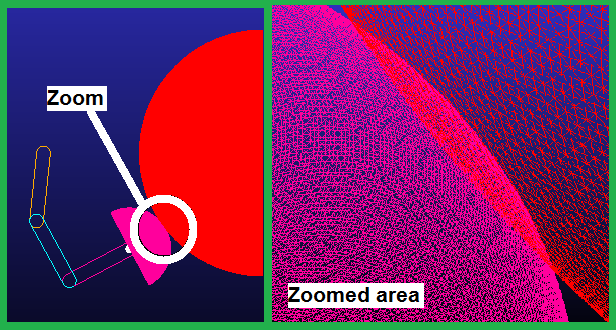
\includegraphics[width=\linewidth]{contacted_mesh.png}%
}{%
\caption{Contact model in Adams.}%
\label{fig:contactedmesh}%
}
\capbtabbox{%
    \begin{tabular}{cccc}
    \toprule
    \textbf{Parameter} & \textbf{Value}\\
    \toprule
    $K_{P_p};K_{D_p}$ & $100;20$\\
    \midrule
    $K_{P_f};K_{D_f};K_{I_f}$ & $10;1;0.1$\\
    \midrule
    Stiffness & 1000$\frac{N}{m}$\\
    \midrule
    Damping & 20$\frac{Ns}{m}$\\
    \bottomrule
    \end{tabular}
}{%
    \caption{Test parameters.}%
    \label{tab:sim_parameters}%
}
\end{floatrow}
\end{figure}


Fig.~\ref{fig:NormCompContForce} shows the track of the normal component of the contact force for the sliding on a plane and a sphere surface. And Fig.~\ref{fig:TangCompForce} shows the track of the normal and tangential force during rolling over the a plane.

\begin{figure}[!t]
\centering
\mbox{
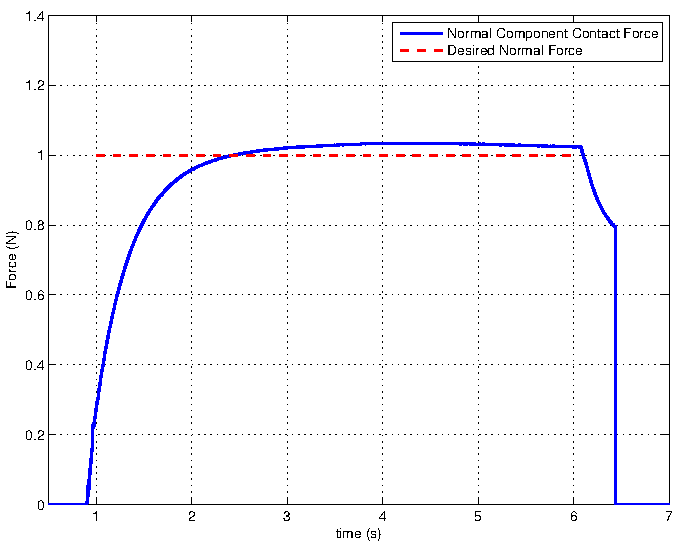
\includegraphics[width=0.45\linewidth]{NormalComponentContactForcePLANE.png}
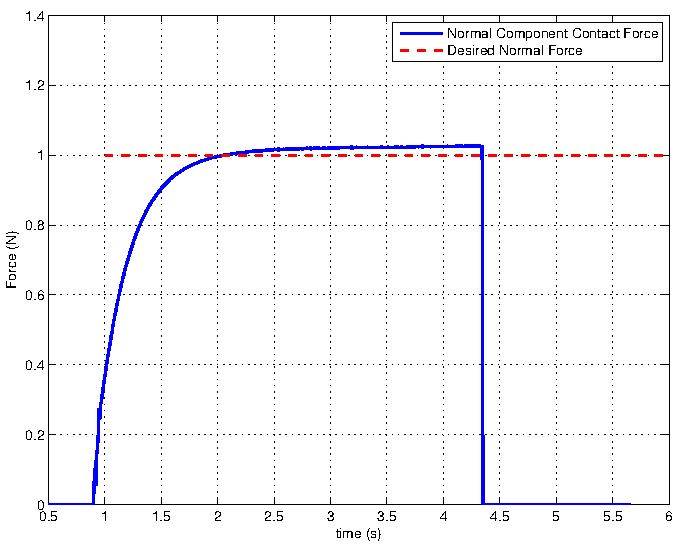
\includegraphics[width=0.45\linewidth]{NormalComponentContactForceSPHERE.png}
}
\caption{Normal component of the contact force when sliding over a plane (left) and a sphere (right).}
\label{fig:NormCompContForce}
\end{figure}

\begin{figure}[!t]
\centering
\mbox{
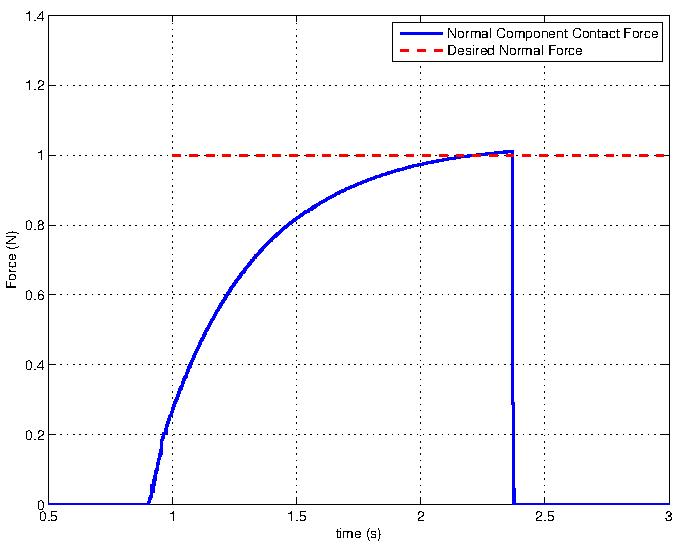
\includegraphics[width=0.45\linewidth]{NormalComponentContactForceROLLPLANE.png}
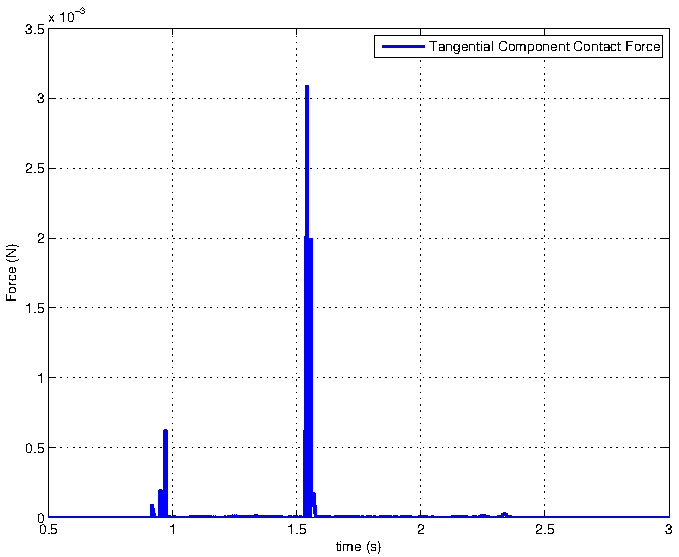
\includegraphics[width=0.45\linewidth]{TangentialComponentContactForceROLLPLANE.png}
}
\caption{Normal (left) and tangential (right) component of the contact force when rolling over a plane.}
\label{fig:TangCompForce}
\end{figure}

The tests were taken to a real scenario shown in Fig.~\ref{fig:curvature}, where the KUKA LWR was equipped with an ATI Nano 17 force torque sensor. The estimated principal curvatures are summarized in Table~\ref{tab:results}. Note that the sphere is a basketball, whose official radius is 11,92-12,07cm, as well as the large values for the plane and one of the pricnipal curvatures on the cylinder.

\begin{table}
\centering
\caption{Experimental Results}
\label{tab:results}
\begin{tabular}{ccccc}
    \toprule
    & \multicolumn{4}{c}{\textbf{Princial Radii}}\\
    \textbf{Object} & \multicolumn{2}{c}{\textbf{Real}} & \multicolumn{2}{c}{\textbf{Estimated}}\\
    \textbf{Direction} & $z$ [m] & $y$ [m] & $z$ [m] & $y$ [m]\\
    \toprule
    Plane & $\infty$ & $\infty$ & 333 & 500 \\
    Cylinder & $\infty$ & .90 & 500 & .088 \\
    Sphere & .1207 & .1207 & 0.121 & 0.127 \\
    \bottomrule
\end{tabular}
\end{table}

\begin{figure}[!h]
    \centering
    \label{fig:curvature}
    \mbox{
    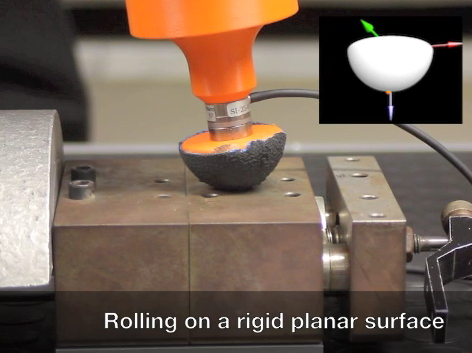
\includegraphics[width=.32\linewidth]{plane}
    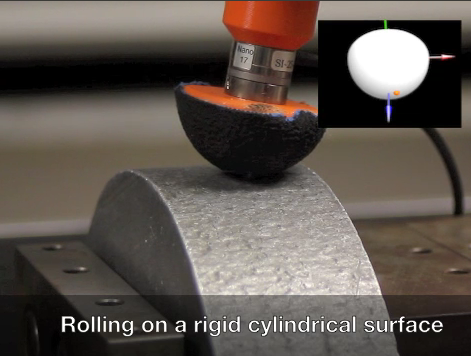
\includegraphics[width=.32\linewidth]{cylinder}
    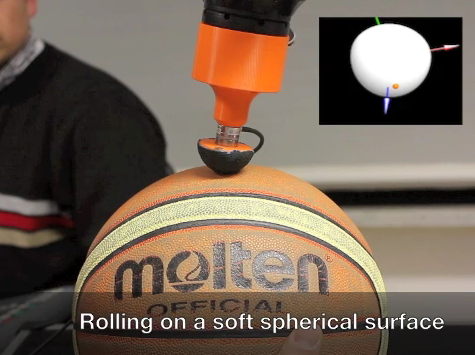
\includegraphics[width=.32\linewidth]{basketball}
    }
    \caption{Test objects for curvature estimation test on a plane (left), a cylinder (middle), and a sphere (right).}
\end{figure}


%This results will be tested again in the new simulation framework presented in~\ref{sec:Simulation}.

\paragraph{(e) Integration of object/part model obtained from vision with the code for reactive haptic exploration strategies}

\begin{figure}[!b]
  \begin{center}
    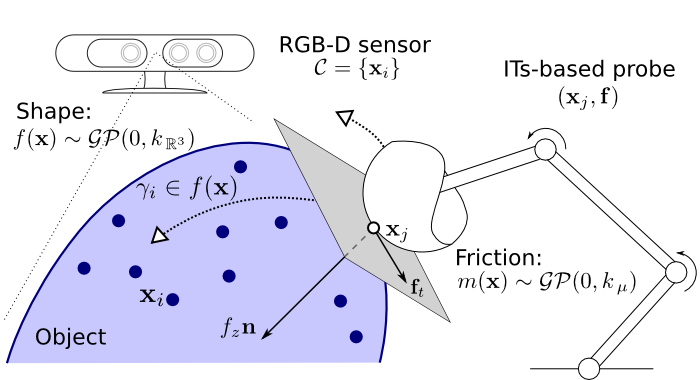
\includegraphics[width=0.95\linewidth]{sliding}
  \end{center}
  \caption{The shape is acquired by an RGBD sensor and the friction coefficients by the intrinsic tactile sensor, both shape~$f(\mathbf{x})$ and friction~$m(\mathbf{x})$ functions are represented as a Gaussian Process $\mathcal{GP}(0,k(\cdot))$. The exploration follows geodesic flows~$\gamma_i$ on the surface of a fixed object using a compliant behavior.}
  \label{fig:schema}
\end{figure}

The setup overview is depicted in Fig.~\ref{fig:schema}. The approach used Gaussian Processes to represent both, shape and fiction coefficient, and it was successfully exploited to generate exploration trajectories on the object surface with arbitrary shapes. The normal contact force was used to discriminate the contact states from the non-contact state. The exploratory probe was the same as in the previous paragraph, with an additional compliant coupler for safety and sensor protection. only sliding controller was used since the friction coefficient is simpler to retrive using that primitive. More details on the whole methodology can be found in the attached paper~\cite{Active2014Rosales} available at~\href{./attachedPapers/ActiveGatheringOfFrictionalPropertiesFromObjects.pdf}{this link}.

% \begin{figure}[th]
%     \centering
%     \mbox{
%         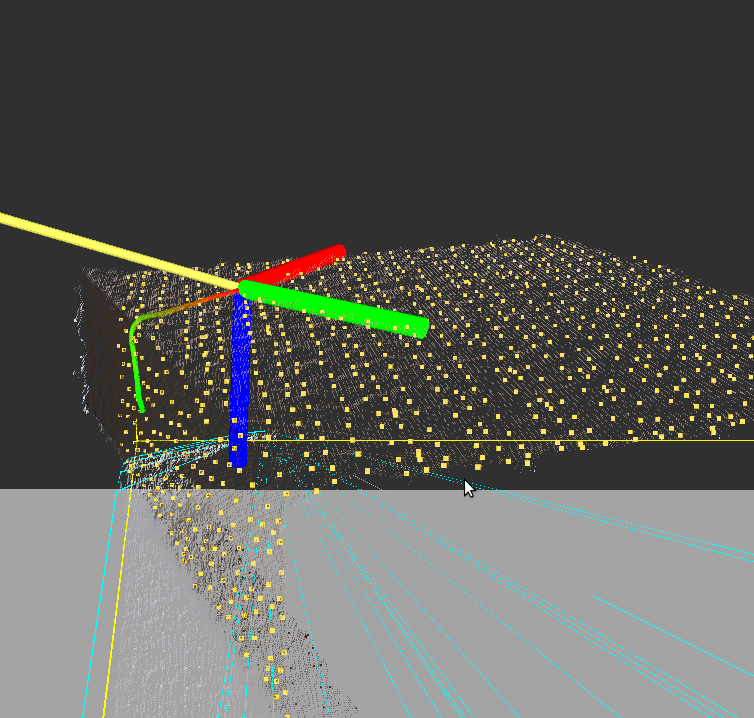
\includegraphics[height=0.4\linewidth]{box.png}
%         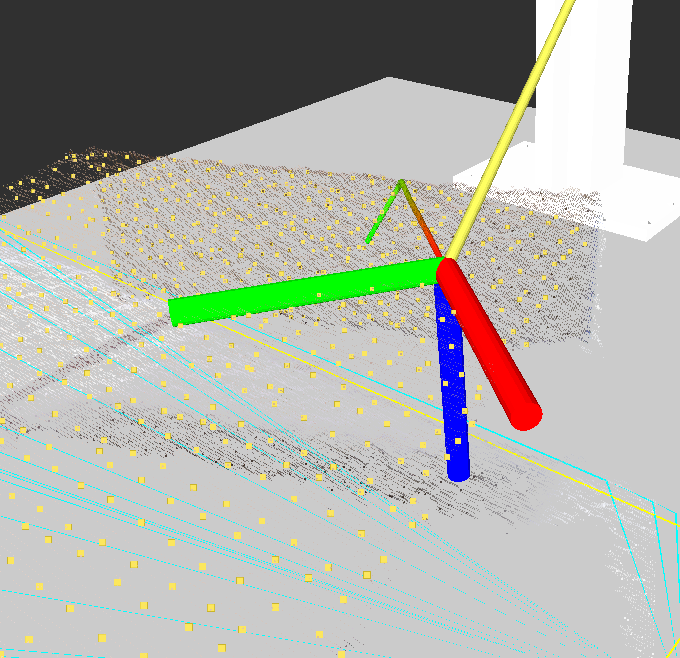
\includegraphics[height=0.4\linewidth]{box1.png}
%         }
%     \mbox{
%         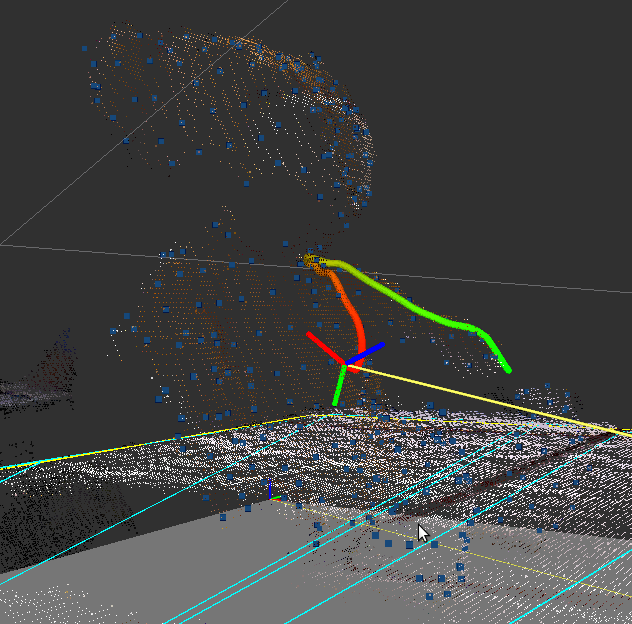
\includegraphics[height=0.4\linewidth]{teddy.png}
%         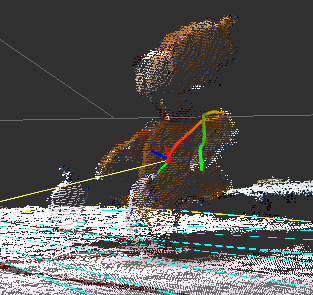
\includegraphics[height=0.4\linewidth]{teddy2.png}
%         }

%     \caption{Geodesic flows on object surfaces captured by an RGBD sensor. The color of the flow goes from red, i.e. the initial contact point, to green, i.e. the final position, according to the predefined length of the curve. The box has flat surfaces, hence geodesics are straight lines (top). The teddy bear has a very irregular shape, but still geodesic flows are found (bottom).}
%     \label{fig:geodesic_examples}
%     \vspace{-0.02\linewidth}
% \end{figure}

% \begin{figure}
%   \centering
%   \mbox{
%         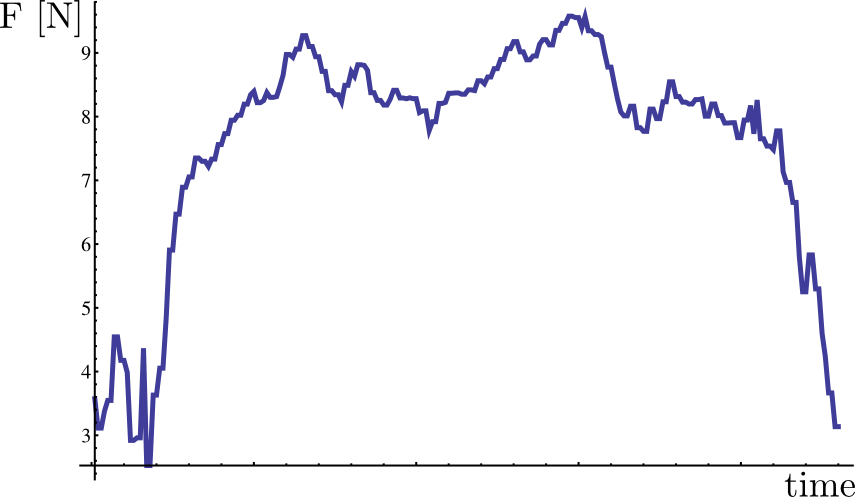
\includegraphics[width=0.45\linewidth]{FZBOX.png}
%         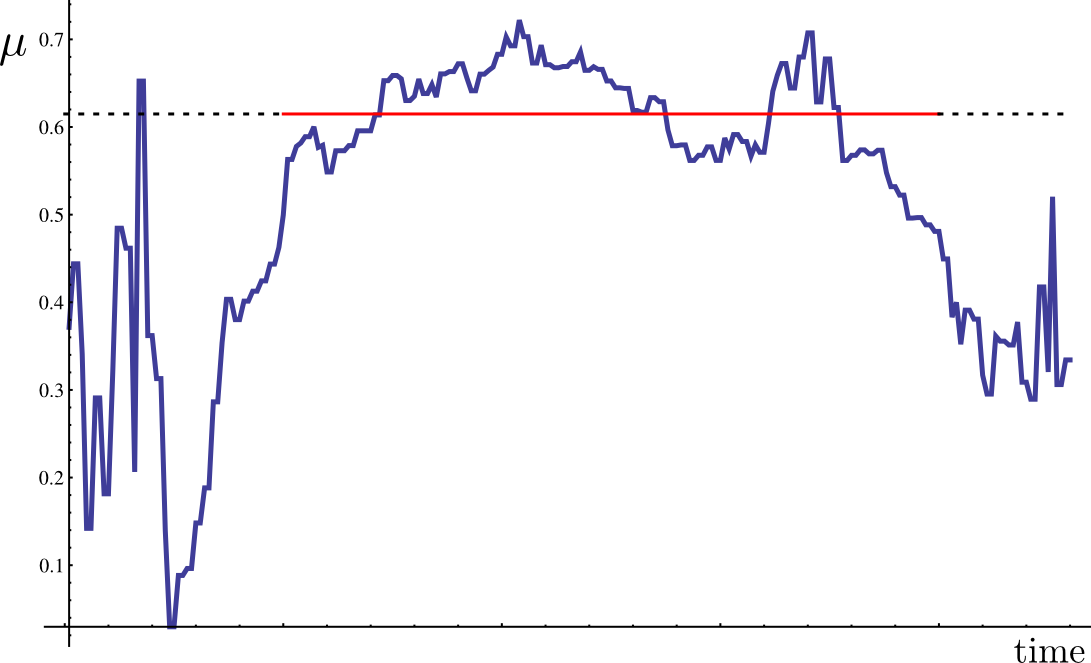
\includegraphics[width=0.45\linewidth]{MuBOX.png}
%         }
%     \caption{Relevant data recorded during a haptic exploration. Force along $\mathbf{z}_{\text{c}}$ used to detect the contact and non-contact states (top). Friction coefficient $\mu$, the red line marks the mean value during the contact state (bottom). Material: Paperboard.}
%     \label{fig:data2}
% \end{figure} 

\subsubsection{Task 3.2}

Previous work on object detection assisted by touch comprise typically fully actuated hands, such as the work presented in~\cite{Bimbo2013Combining}. To this end, the initial estimate provided by the visual input must be of high accuracy in order to place precisely the finger areas covered with tactile arrays. This implies solving the object recognition problem as well. In a extreme case, where no visual input is available, the remarkable work by~\cite{Petrovskaya2011Global} propose a Bayesian approach termed Scaling Series, however, the testbed was a robot arm equipped with a single force/torque sensor which allow to compute with high accuracy the contact point w.r.t. to the robot base. The inconvenient of such setup the probing. As said in the paper, each probe took approximately $10$s, and in the meantime, the algorithm, which is not light, was allowed to do computations. 

Thus, the fact that the object shape and localization uncertainty is reduced by making contact, combined with the adaptability of the Pisa/IIT SoftHand to any object shape, influenced the idea of using the hand as sophisticated exploratory probe w.r.t. previous testbeds. The configuration is similar to the usual adopted in bio-mechanic systems~\cite{Cappozzo1995}, direct sensorization of the limbs is advised via optical or magnetic markers, or inertial devices, ``strap down'' to the greatest extent to the underlying bone, while defining the simplest assembly of technical joints that best reproduces the animal or human joint motion~\cite{Lucchetti1998}. We propose a glove-inspired inertial-based solution to read the hand configuration for object detection as the result of a grasping action.%, and correlate motion patterns to functional status levels for clinical studies~\cite{Balzini2003}

We strongly believe that the proposed solution will be of great help in situations where partial or none visual information is available, as challenged in Task 3.2. Thus, we dedicated efforts to continue on this research as it seems beneficial to accomplish the project goals with an alternative methodology than the initially proposed. The following two paragraphs show the preliminary and on-going positive results on this topic, respectively.


%%%%%%%%%%%%%%%%%%%%%%%%%%%%%%%%%%%%%%%%%%%%%%%%%%%%%%%%%%%%%%%%%%%%%%%%%%%%%%

% To be prepared by: Marco Gabiccini
% Low-cost, Fast and Accurate Reconstruction of Robotic and Human Postures
% via IMU Measurements
%%% Low-cost, Fast and Accurate Reconstruction of Robotic and Human Postures
%%% via IMU Measurements

\subsubsection{Low-cost, Fast and Accurate Reconstruction of Robotic and Human Postures via IMU Measurements} 

In this section, we describe our approach to reconstruct the posture of kinematic structures which do not easily lend themselves to the use of rotary encoders. This part is motivated by our need to measure the joint angles of the Pisa/IIT SofHand --- its particular joint structure does not allow to fit encoders ---  after it has wrapped around an object (e.g., in an enveloping grasp), for the sake of employing it as a probe to explore and recognize objects.
 
The above discussed need, along with the mentioned constraints, brought us to consider the general problem of reconstructing the configurations of kinematic trees of rigid bodies without using measurements of relative angles, but employing absolute attitude sensors, such as IMUs, along with suitable filter algorithms. We argue that the relatively larger inaccuracies shown by absolute sensors can be compensated by suitable processing, such as passive complementary filters exploiting the Mahony-Hamel formulation. The proposed method is applicable to general kinematic structures where measurements of relative angles is not feasible or convenient, or where, as in the case of the Pisa/IIT SoftHand, the joint kinematics are not lower pairs. In the accompanying paper~\cite{Santaera:ICRA:2015} we present quantitative comparisons with ground truth data in grasping tests obtained for a two-fingered gripper: here, the fingers share the very same kinematic structure of that of the Pisa/IIT SoftHand. The comparisons validate the method employed, testifying that the resulting hardware design is mechanically robust, cheap and can be easily adapted to robotic hands with different topology, as well as to sensorizing gloves for studying human grasping strategies.

More details on this new approach and on the achieved results can be found in the attached paper~\cite{Santaera:ICRA:2015} available at this~\href{./attachedPapers/ReconstructionPosturesImuMeasurements.pdf}{link}.  

%%%%%%%%%%%%%%%%%%%%%%%%%%%%%%%%%%%%%%%%%%%%%%%%%%%%%%%%%%%%%%%%%%%%%%%%%%%%%%

% To be prepared by: Gaspare and Emanuele
% Endowing the Pisa/IIT SoftHand with the sense of touch
%%%% Endowing the Pisa/IIT SoftHand with the sense of touch

\subsubsection{Endowing the Pisa/IIT SoftHand with the sense of touch}
\label{sec:SenseOfTouch}


\paragraph{(a) The Madgwick Filter}

%\noindent $\blacktriangleright$  \textbf{The Madgwick Filter} \\
%\newline


In~\cite{Santaera:ICRA:2015} a modified version of the Mahony-Hamel passive complementary filter was used to obtain the orientation of a generic frame $\{ A \}$ with respect to frame $\{ B \}$, expressed by a rotation matrix.

In his works, Sebastian Madgwick~\cite{MadgwickMARG} studied a new algorithm able to better use measurements read by sensors. The algorithm proposed is also able to tackle the singularities, associated for example with Euler angle representation, by employing quaternions to represent a general orientation. The Madgwick filter is similar to Mahony-Hamel filter in that, at each time step, a new orientation quaternion is estimated summing, to its previous estimation, a correction factor that depends on the data read from an IMU.

Let be ${^b\omega_x}$, ${^b\omega_y}$ and ${^b\omega_z}$ angular rate measures (in $\rad s^{-1}$) with respect the IMU body frame $\{ B\}$ respectively about $x$, $y$ and $z$ axis and $^{b}\Omega$ a vector containing these measures as
\begin{equation}
\label{eq4_01}
^b \Omega = [ 0 \quad {^b\omega_x} \quad {^b\omega_y} \quad {^b\omega_z} ],
\end{equation}

\noindent the quaternion describing the rate of change of the earth frame $\{ A \}$ with respect to the sensor frame $\{ B \}$ can be written as

\begin{equation}
\label{eq4_02}
^b_a\dot{q} = \frac{1}{2} {^b_a \bar{q}}  \otimes {^b\Omega}.
\end{equation}

\noindent Where $\otimes$ denotes a quaternion product, while $\bar{}$ denotes the (unity) normalization operator. From eq.~\eqref{eq4_02} trivially the orientation of the earth frame with respect to sensor frame at time \textit{t} is given by eq. (\ref{eq4_03}) and (\ref{eq4_04}) as

\begin{equation}
\label{eq4_03}
^b_a \dot{q}_{\Omega,t} = \frac{1}{2} {^b_a \hat{\bar{q}}_{t-1}} \otimes ^b \Omega_t,
\end{equation}

\begin{equation}
\label{eq4_04}
^b_a q_{\Omega,t} = {^b_a \hat{\bar{q}}_{t-1}} + {^b_a \dot{q}_{\Omega,t}} \Delta t,
\end{equation}

\noindent where $^b \Omega_t$ is angular rate measured at time \textit{t}, $\Delta t$ is the sampling period and $^b_a \hat{\bar{q}}_{t-1}$ is the previous estimate of the orientation quaternion.

Now, by reading from a sensor a set of accelerometer and compass measurements in a frame strap down to the sensor, one can find infinite earth frame orientations, according to measures read from the sensors.
However, using quaternions to express an orientation, it is very easy to overcome the singularity problem, obtaining from sensors measures an unique orientation for the earth frame with respect the one attached to the sensor.
From this considerations, the orientation problem can be written as an optimization problem, where quaternion $^b_a \bar{q}$ aligns a predefined reference direction of a field (gravity or magnetic) in the earth frame $^a \bar{d}$, with the measured direction of the field in the sensor frame $^b \bar{s}$. Therefore, the quaternion $^b_a \bar{q}$ is given by the problem

\begin{equation}
\label{eq4_05}
\min_{{^b_a \bar{q}} \in \mathbb{R}^4} f({^b_a \bar{q}}, {^a \bar{d}}, {^b \bar{s}}),
\end{equation}

\noindent with the objective function $f$, $^b_a \bar{q}$ and the vectors $^a \bar{d}$ and $^b \bar{s}$ defined as

\begin{equation}
\label{eq4_06}
f(^b_a \bar{q},^a \bar{d}, ^b \bar{s}) = ^b_a \bar{q}^{*} \otimes ^a \bar{d} \otimes ^b_a \bar{q} - ^b \bar{s},
\end{equation}

\begin{equation}
\label{eq4_07}
^b_a \bar{q} = [q_1 \quad q_2 \quad q_3 \quad q_4],
\end{equation}

\begin{equation}
\label{eq4_08}
^a \bar{d} = [0 \quad d_x \quad d_y \quad d_z],
\end{equation}

\begin{equation}
\label{eq4_09}
^b \bar{s} = [0 \quad s_x \quad s_y \quad s_z],
\end{equation}

\noindent and $^{*}$ in (\ref{eq4_06}) denotes the conjugate operator of a quaternion $q = [q_1 \quad q_2 \quad q_3 \quad q_4]$ as $q^* = [q_1 \quad -q_2 \quad -q_3 \quad -q_4]$. To solve problem in (\ref{eq4_05}) many algorithms can be used. However, for the problem at hand, a gradient descent strategy appeared a satisfactory choice in terms of low computational burden and efficiency. With this choice and starting from an initial (guess) quaternion $^b_a \bar{q}_0$, it is possible to write the quaternion correction factor $^b_a \bar{q}_{k+1}$ linked to step $(k+1)^{th}$ as follows

\begin{equation}
\label{eq4_10}
^b_a q_{k+1} = ^b_a \bar{q}_k - \beta \frac{\nabla f(^b_a \bar{q}_k, ^a \bar{d}, ^b \bar{s})}{\vert \vert \nabla f(^b_a \bar{q}_k, ^a \bar{d}, ^b \bar{s}) \vert \vert}, \quad k = 0,1,2 \dots n,
\end{equation}

\noindent where
\begin{equation}
\label{eq4_10bis}
^b_a \bar{q}_k = \frac{1}{2} {^b_a \bar{q}_{k-1}} \otimes ^b{\Omega_k},  \quad k = 1,2,3 \dots n,
\end{equation}

\begin{equation}
\label{eq4_11}
\nabla f(^b_a \bar{q}_k, ^a \bar{d}, ^b \bar{s}) = J^T(^b_a \bar{q}_k,^a \bar{d}) f(^b_a \bar{q}_k, ^a \bar{d}, ^b \bar{s}),
\end{equation}

\begin{equation}
\label{eq4_12}
\begin{split}
f(^b_a \bar{q}_k, ^a \bar{d}, ^b \bar{s}) =
\left [ \begin{array}{c}
2d_x(\frac{1}{2} - q_3^2 - q_4^2) + 2d_y(q_1q_4 + q_2 q_3) + \\
2d_x(q_2 q_3 - q_1 q_4) + 2d_y(\frac{1}{2} - q_2^2 - q_4^2) + \\
2d_x(q_1 q_3 + q_2 q_4) + 2d_y(q_3 q_4 - q_1 q_2) + \end{array} \right. \\
\left. \begin{array}{r}
2 d_z(q_2q_4 - q_1q_3) - s_x \\
2d_z(q_1q_2 + q_3 q_4) - s_y \\
2d_z(\frac{1}{2} - q_2^2 - q_3^2) - s_z
\end{array} \right ] \end{split},
\end{equation}

\begin{equation}
\label{eq4_13}
\begin{split}
J(^b_a \bar{q}_k, ^a \bar{d}) =
\left [ \begin{array}{cc}
2d_yq_4 - 2d_zq_3 & 2d_yq_3+ 2d_zq_4\\
-2d_xq_4 + 2d_zq_2 & 2d_xq_3 - 4d_yq_2 + 2d_zq1 \\
2d_xq_3 - 2d_yq_2 & 2d_xq_4 - 2d_yq_1 - 4d_zq_2 \end{array} \right. \\
\left. \begin{array}{rr}
-4d_x q_3 2d_y q_2 - 2d_z q_1 & -4d_x q_4 2d_y q_1 + 2d_z q_2\\
2d_x q_2 + 2d_z q_4 &  -2d_x q_1 - 4d_y q_4 + 2d_z q_3\\
2d_x q_1 + 2 d_y q_4 - 4 d_z q_3 & 2 d_x q_2 + 2d_y q_3
\end{array} \right ] \end{split},
\end{equation}

\noindent where $\beta$ denotes the step size, while $J^T$ denotes the transpose of the Jacobian matrix of the objective function $f$.

Problem described in eq. (\ref{eq4_05}) is a general alignement problem. Therefore, by considering measurements read from accelerometers and from magnetormeters, it is possible to write two different problems: the first one from accelerometers data $f_g(^b_a \overline{q}_k, ^a \overline{g}_a, ^b \overline{g}_b)$ where $^a\overline{g}_a = \overline{g}_a$ is the gravity field measured in the inertial frame while $^b \overline{g}_b = \overline{g}_b$ is the gravity field in the sensor frame; in a similar manner, the second problem is $f_m(^b_a \overline{q}_k, ^a \overline{m}_a, ^b \overline{m}_b)$ with $^a\overline{m}_a = \overline{m}_a$ magnetic field read in the inertial frame and $^s \overline{m}_b = \overline{m}_b$ magnetic field read in the sensor frame.
Combining the two optimization problems as follows

\begin{equation}
\label{eq4_14}
f_{g,m}(^b_a \overline{q},\overline{g}_a,\overline{g}_b,\overline{m}_a,\overline{m}_b) = \left [ \begin{array}{c} f_g(^b_a \overline{q}, \overline{g}_a, \overline{g}_b) \\  f_m(^b_a \overline{q},  \overline{m}_a,  \overline{m}_b) \end{array} \right ],
\end{equation}

\noindent it is possible to find an unique quaternion which describes the orientation, at step $(k+1)^{th}$, of the inertial frame with respect the sensor frame as

\begin{equation}
\label{eq4_15}
^b_a q_{k+1} = ^b_a \overline{q}_k - \beta \frac{\nabla f_{g,m}(^b_a \overline{q}_k,\overline{g}_a,\overline{g}_b,\overline{m}_a,\overline{m}_b) }{\vert \vert \nabla f_{g,m}(^b_a \overline{q}_k,\overline{g}_a,\overline{g}_b,\overline{m}_a,\overline{m}_b)  \vert \vert}, \quad k = 0,1,2 \dots n,
\end{equation}

\noindent with

\begin{equation}
\begin{split}
\label{eq4_16}
\nabla f_{g,m}(^b_a \overline{q}_k,\overline{g}_a,\overline{g}_b,\overline{m}_a,\overline{m}_b) = J_{g,m}^T(^b_a \overline{q}_k, \overline{g_a},\overline{m_a}) \\ {f}_{g,m}(^b_a \overline{q}_k,\overline{g}_a,\overline{g}_b,\overline{m}_a,\overline{m}_b),
\end{split}
\end{equation}

\noindent and

\begin{equation}
\label{eq4_17}
J_{g,m}^T(^b_a \overline{q}_k, \overline{g_a}, \overline{m_a}) = \left [ \begin{array}{c} J_g(^b_a \overline{q}_k,\overline{g}_a) \\ J_m(^b_a \overline{q}_k, \overline{m}_a) \end{array} \right ]
\end{equation}

\noindent where $J_g$ and $J_m$ respectvily the Jacobians of the function $f_g$ and $f_m$.

In Figure~\ref{BlockDiagram}, the block diagram of the Madgwick filter is depicted. Algorithm~\ref{MadgwickAlg} details the steps followed to obtain the orientation quaternion using its previous estimation and the data read from IMU, using $g_a$ and $m_a$ to denote, respectively, the gravity and the magnetic field in the inertial frame. In particular, the gravity field is commonly set as $g_a = [0 \quad 0 \quad 0 \quad 1]$, or rather, using a North-East-Down convention. The earth magnetic field can be considered to have two components: one along the horizontal axis and one in the vertical axis, with its vertical component due to the inclination of the field depending by the latitude. In Pisa, for example, it is about $1\degree$ w.r.t. the horizontal, so $m_a = [0 \quad m_{a_x} \quad 0 \quad m_{a_z}]$.

\begin{figure}[t]
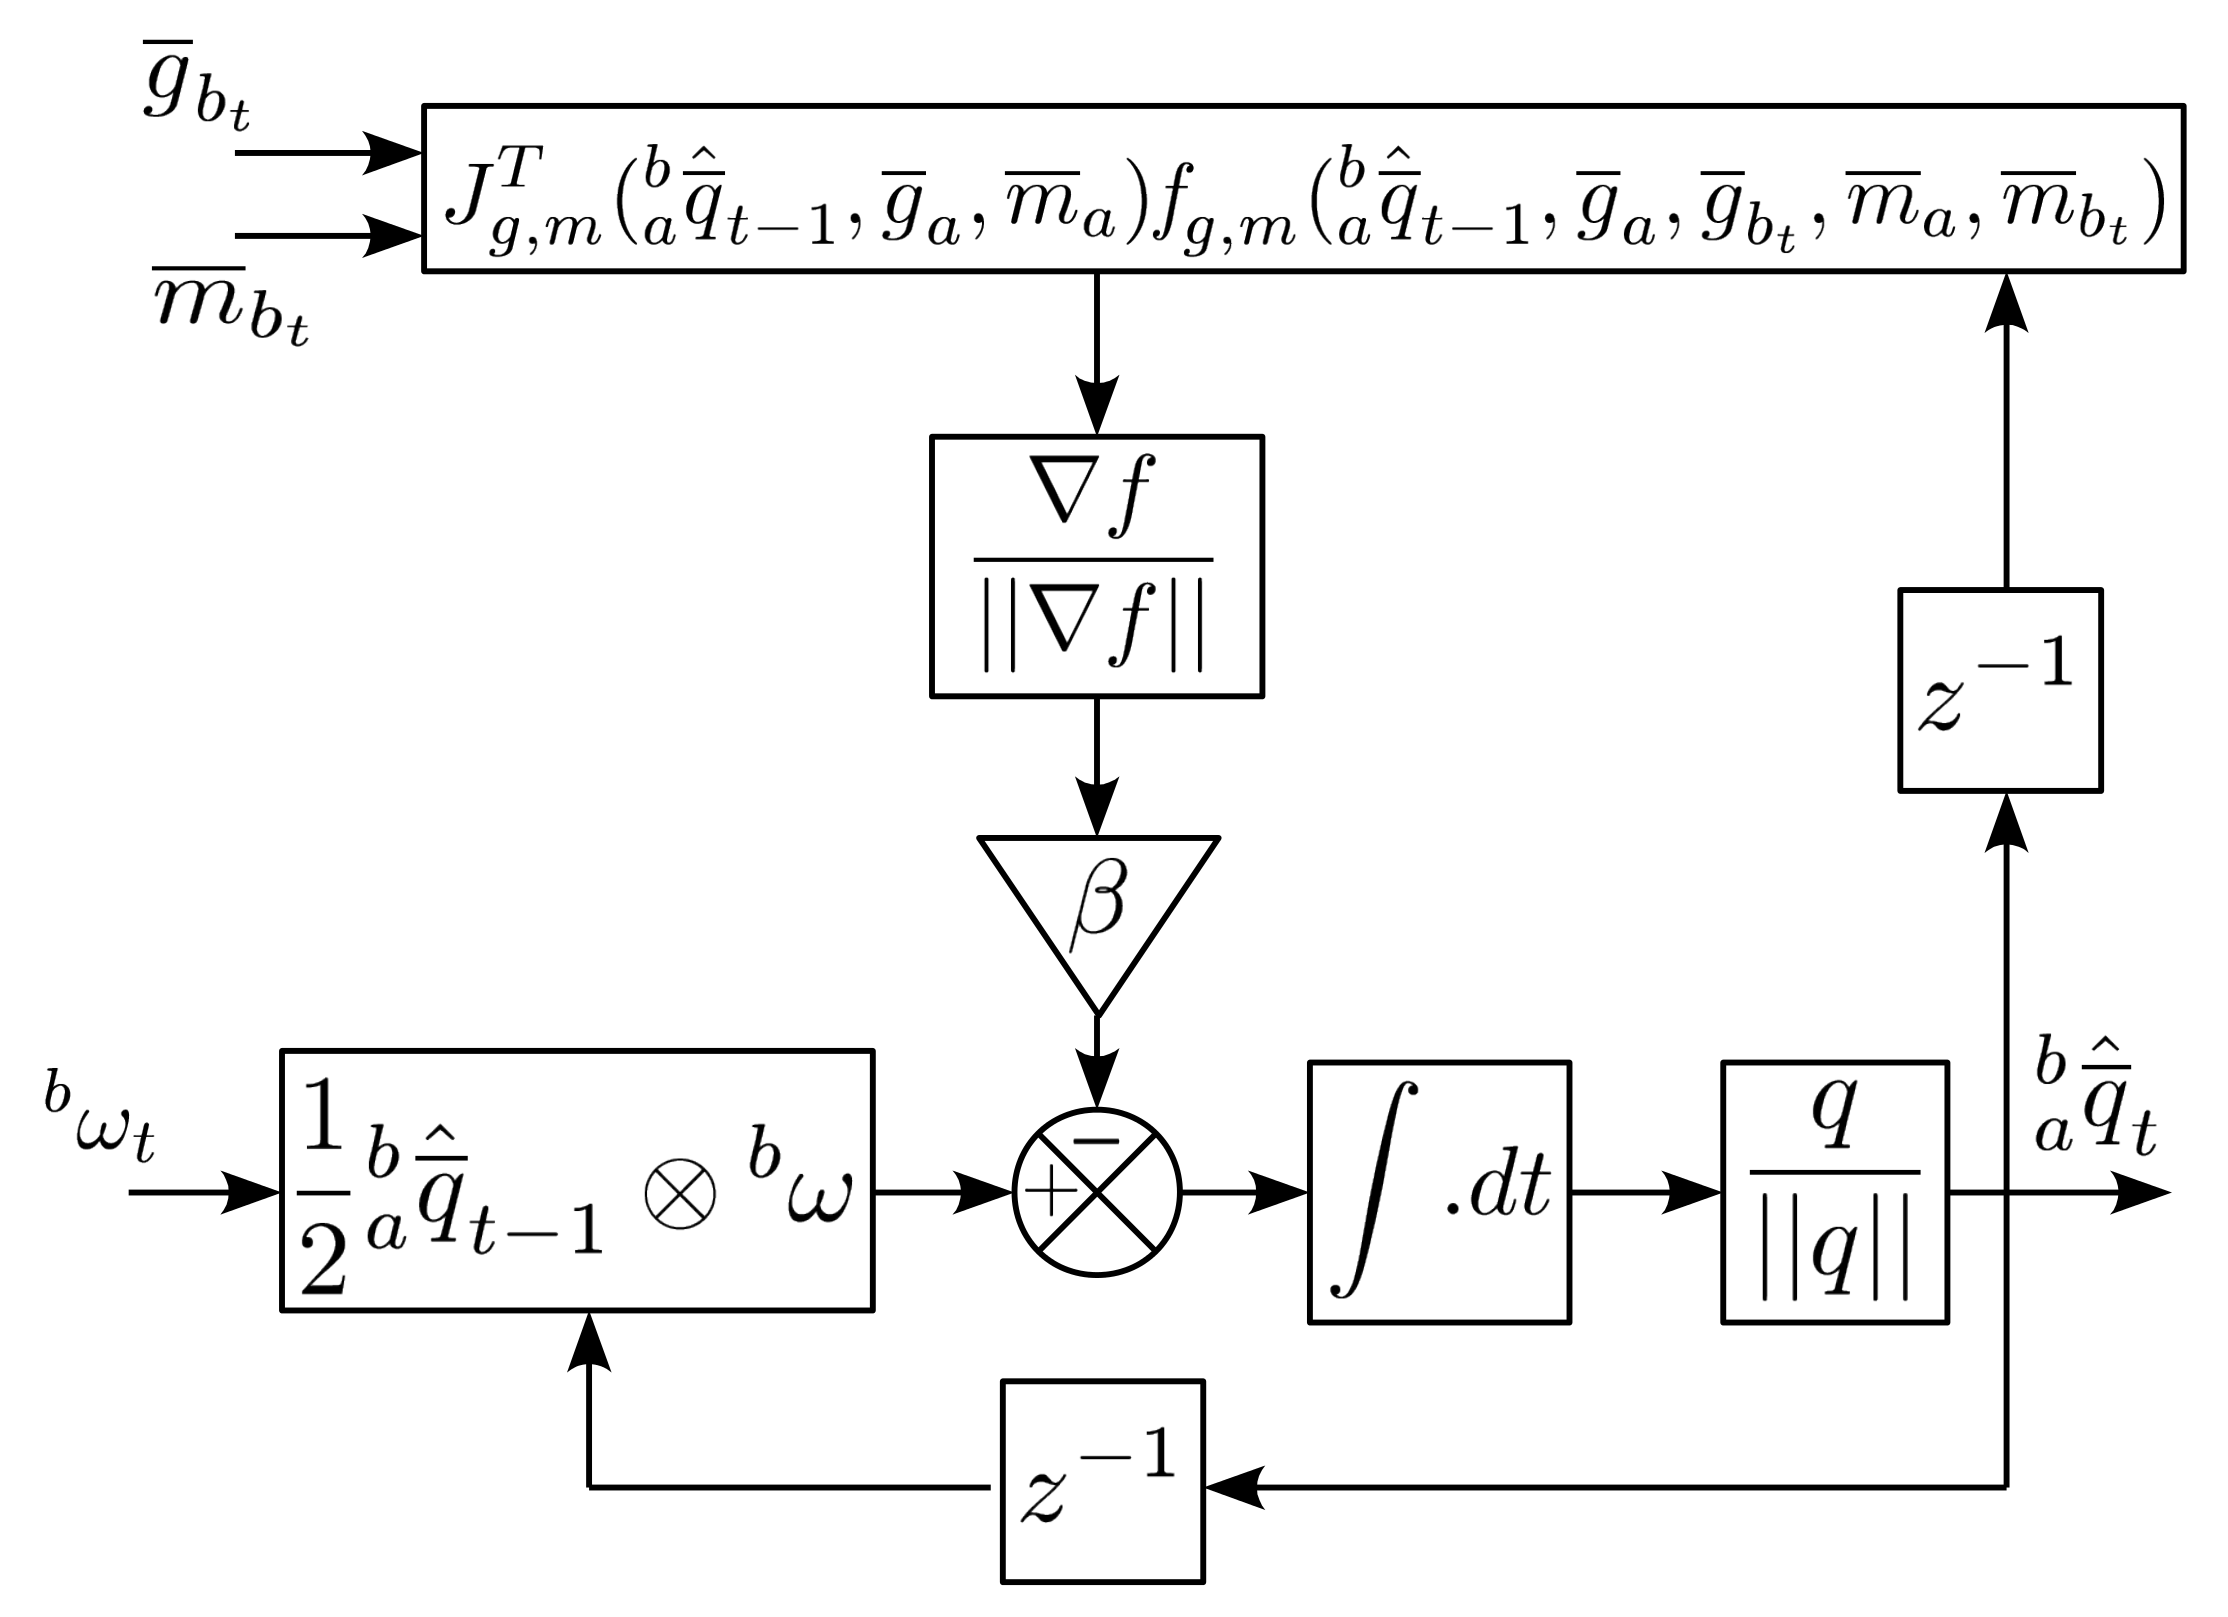
\includegraphics[scale=0.45]{Madgwick_Block_Diagram}
\caption{Block diagram of the Madgwick passive complementary filter}
\label{BlockDiagram}
\end{figure}

\begin{algorithm}
\caption{Madgwick Discrete Filter at $n^{th}$ step}
\begin{algorithmic}[1]
\label{MadgwickAlg}
\STATE Reading the current values of the accelerometers ($g_{b_n}$), magnetometers ($m_{b_n}$) and gyro rates ($\Omega_{b_n}$) in the local IMU frame $\{B\}$
\STATE Normalizing gravity and magnetic field vector read from IMU $\overline{g}_{b_n} = \frac{g_{b_n}}{\vert \vert g_{b_n} \vert \vert}$, $\overline{m}_{b_n} \frac{m_{b_n}}{\vert \vert m_{b_n} \vert \vert}$
\STATE Computing the objective function value $f_{g,m}({^b_a\hat{\overline{q}}_{n-1}},\overline{g}_a,\overline{g}_{b_n},\overline{m}_a,\overline{m}_{b_n})$ using equations (\ref{eq4_12}) and (\ref{eq4_14})
\STATE Computing the transpose of the Jacobian of the objective function $J^T_{g,m}(^b_a\hat{\overline{q}}_{n-1},\overline{g_a},\overline{m}_a)$ using equations (\ref{eq4_13}) and (\ref{eq4_17})
\STATE Computing the correction terms $c_n =  \beta \frac{\nabla f}{\vert \vert \nabla f \vert \vert}$ using equation (\ref{eq4_16})
\STATE Computing the orientation quaternion time variation $^b_a \hat{q}_{d_n} =  (\frac{1}{2} {^b_a\hat{\overline{q}}_{n-1}} \otimes \Omega_{b_n}) - c_n$
\STATE Computing the new orientation quaternion estimation given by its previouly one and its current time variation $^b_a \hat{q}_n = ^b_a\hat{\overline{q}}_{n-1} + ^b_a \hat{q}_{d_n} \Delta t$
\STATE Normalizing the new estimated quarternion $^b_a \hat{\overline{q}}_n = \frac{^b_a \hat{q}_n}{\vert \vert ^b_a \hat{q}_n \vert \vert}$
\end{algorithmic}
\end{algorithm}

\begin{figure}[t]
\centering
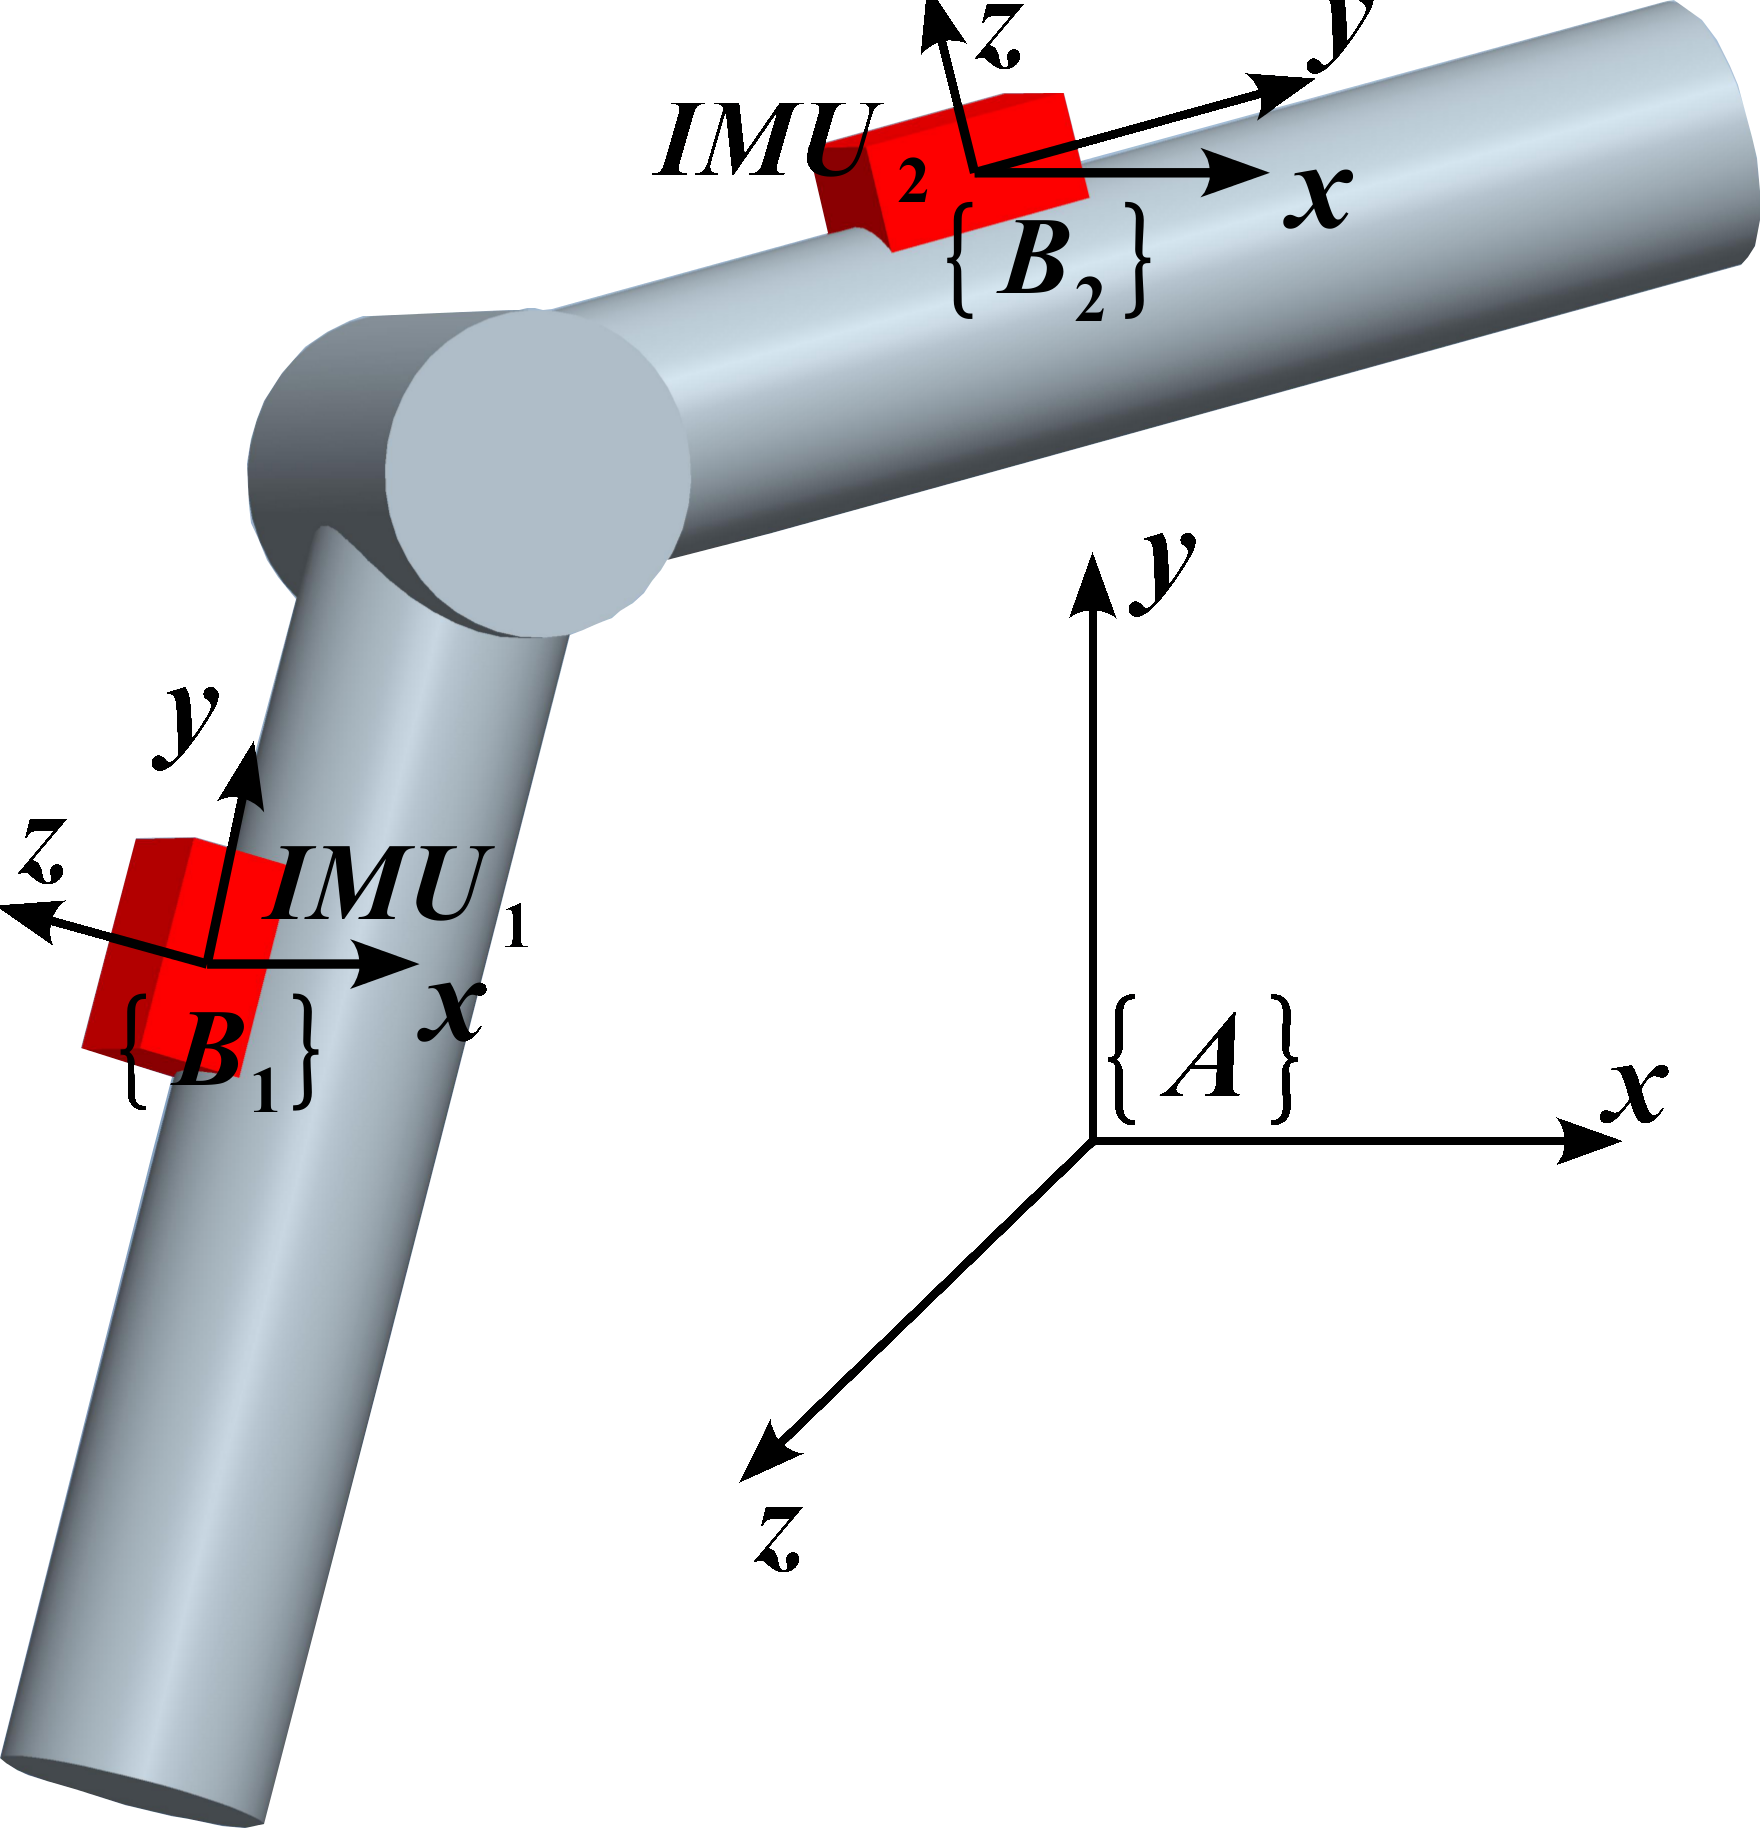
\includegraphics[scale=0.5]{TwoLinksOneJoint.png}
\caption{Simple structure with two link connected by a revolute joint}
\label{TwoLinksOneJoint}
\end{figure}

\subparagraph{Orientation between two IMUs}
%\noindent $\bullet$ \textbf{Orientation betwenn two IMUs}

When employing two different IMUs in a configuration as shown in Figure~\ref{TwoLinksOneJoint}, these will return two different sets of measurements ($r_1,r_2$) referred to their body frame $\{ B_1 \}$ and $\{ B_2 \}$. Applying the Madgwick filter to $r_1$, one will get $^{b{_1}}_a \hat{\overline{q}}$ or, rather, the orientation quaternion of the inertial frame with respect to frame $\{ B_1 \}$, while from $r_2$ the filter will return $^{b{_2}}_a \hat{\overline{q}}$ or, rather, the orientation quaternion of the inertial frame with respect to frame $\{ B_2 \}$. Trivially, the orientation quaternion of the frame $\{ B_2 \}$ with respect the frame $\{ B_1 \}$ is given by

\begin{equation}
\label{eq4_18}
{^{b_1}_{b_2}\hat{\overline{q}}} = {_{a}^{b_2}\hat{\overline{q}}^{*}} \otimes {_{a}^{b_1}\hat{\overline{q}}}.
\end{equation}

However, as seen for the Mahony-Hamel filter, it is possible to apply in a suitable way the Madgwick filter to data read from the two IMUs, to obtain ${^{b_1}_{b_2}\hat{\overline{q}}}$.

Starting from the IMUs measurements where $\overline{g}_{b_1}$, $^{b_1} \Omega$ and $\overline{m}_{b_1}$ denotes respectively accelerometer, gyroscope and magnetometer measurements in $\{ B_1 \}$,  while $\overline{g}_{b_2}$, $^{b_2} \Omega$ and $\overline{m}_{b_2}$ denotes respectively accelerometer, gyroscope and magnetometer measurements in $\{ B_2 \}$, the first term of the correction factor (\ref{eq4_10}), as written in (\ref{eq4_10bis}), becomes

\begin{equation}
\label{eq4_19}
^{b_1}_{b_2} \bar{q}_k = \frac{1}{2} {^{b_1}_{b_2} \bar{q}_{k-1}} \otimes {^{b_1}_{b_2} \Omega_k},  \quad k = 1,2,3 \dots n,
\end{equation}

\noindent where

\begin{equation}
\label{eq4_20}
{^{b_1}_{b_2} \Omega_k} = {^{b_2} \Omega_k} - {^{b_1}_{b_2} \bar{q}_{k-1}} \otimes {^{b_1} \Omega_k} \otimes {^{b_1}_{b_2} \bar{q}^{*}_{k-1}},
\end{equation}

\noindent is the angular rate of frame $\{ B_2 \}$ (attached to the $\text{IMU}_2$) with respect the frame $\{ B_1 \}$ (attached to $\text{IMU}_1$). The second term of the correction factor, in (\ref{eq4_16}), becomes

\begin{equation}
\begin{split}
\label{eq4_21}
\nabla f_{g,m}(^{b_1}_{b_2} \bar{q}_k,\bar{g}_{b_2},\bar{g}_{b_1},\bar{m}_{b_2},\bar{m}_{b_1}) = J_{g,m}^T(^{b_1}_{b_2} \bar{q}_k, \bar{g_{b_2}},\bar{m_{b_2}}) \\ {f}_{g,m}(^{b_1}_{b_2} \bar{q}_k,\bar{g}_{b_2},\bar{g}_{b_1},\bar{m}_{b_2},\bar{m}_{b_1}).
\end{split}
\end{equation}

\noindent Thus, the orientation quaternion of the frame $\{ B_2 \}$, with respect the frame ${\{ B_1 \}}$, at step $(k+1)^{th}$, is given by

\begin{equation}
\label{eq4_22}
^{b_1}_{b_2} q_{k+1} = ^{b_1}_{b_2} \bar{q}_k - \beta \frac{\nabla f_{g,m}(^{b_1}_{b_2} \bar{q}_k,\bar{g}_{b_2},\bar{g}_{b_1},\bar{m}_{b_2},\bar{m}_{b_1}) }{\vert \vert \nabla f_{g,m}(^{b_1}_{b_2} \bar{q}_k,\bar{g}_{b_2},\bar{g}_{b_1},\bar{m}_{b_2},\bar{m}_{b_1})  \vert \vert}, \quad k = 0,1,2 \dots n.
\end{equation}

In algorithm~\ref{MadgwickAlgTwo} the steps followed to obtain the orientation quaternion of a frame $\{ B_2 \}$ with respect frame $\{ B_1 \}$ are presented.

\begin{algorithm}
\caption{Two IMUs Madgwick Discrete Filter at $n^{th}$ step}
\begin{algorithmic}[1]
\label{MadgwickAlgTwo}
\STATE Reading the current values of the accelerometers ($g_{{b_1}_n}$), magnetometers ($m_{{b_1}_n}$) and gyro rates ($\Omega_{{b_1}_n}$) in the local $IMU_1$ frame $\{B_1\}$
\STATE Normalizing gravity and magnetic field vector read from $IMU_1$ $\overline{g}_{{b_1}_n} = \frac{g_{{b_1}_n}}{\vert \vert g_{{b_1}_n} \vert \vert}$, $\overline{m}_{{b_1}_n} \frac{m_{{b_1}_n}}{\vert \vert m_{{b_1}_n} \vert \vert}$
\STATE Reading the current values of the accelerometers ($g_{{b_2}_n}$), magnetometers ($m_{{b_2}_n}$) and gyro rates ($\Omega_{{b_2}_n}$) in the local $IMU_2$ frame $\{B_2\}$
\STATE Normalizing gravity and magnetic field vector read from $IMU_2$ $\overline{g}_{{b_2}_n} = \frac{g_{{b_2}_n}}{\vert \vert g_{{b_2}_n} \vert \vert}$, $\overline{m}_{{b_2}_n} \frac{m_{{b_2}_n}}{\vert \vert m_{{b_2}_n} \vert \vert}$
\STATE Computing the objective function value $f_{g,m}({^{b_1}_{b_2}\hat{\overline{q}}_{n-1}},\overline{g}_{{b_2}_n},\overline{g}_{{b_1}_n},\overline{m}_{{b_2}_n},\overline{m}_{{b_1}_n})$ using equations (\ref{eq4_12}) and (\ref{eq4_14})
\STATE Computing the transpose of the Jacobian of the objective function $J^T_{g,m}(^{b_1}_{b_2}\hat{\overline{q}}_{n-1},\overline{g}_{{b_2}_n},\overline{m}_{{b_2}_n})$ using equations (\ref{eq4_13}) and (\ref{eq4_17})
\STATE Computing the correction terms $c_n =  \beta \frac{\nabla f}{\vert \vert \nabla f \vert \vert}$ using equation (\ref{eq4_16})
\STATE Computing the orientation quaternion time variation $^{b_1}_{b_2} \hat{q}_{d_n} =  (\frac{1}{2} {^{b_1}_{b_2}\hat{\overline{q}}_{n-1}} \otimes {^{b_1}_{b_2} \Omega_k}) - c_n$ using (\ref{eq4_20})
\STATE Computing the new orientation quaternion estimation given by its previouly one and its current time variation $^{b_1}_{b_2} \hat{q}_n = ^{b_1}_{b_2}\hat{\overline{q}}_{n-1} + ^{b_1}_{b_2} \hat{q}_{d_n} \Delta t$
\STATE Normalizing the new estimated quarternion $^{b_1}_{b_2} \hat{\overline{q}}_n = \frac{^{b_1}_{b_2} \hat{q}_n}{\vert \vert ^{b_1}_{b_2} \hat{q}_n \vert \vert}$
\end{algorithmic}
\end{algorithm}

\paragraph{(b) Hardware}

In this section, the sensors used are described along with their interrogation and management by the filter. Information about acceleration, angular rate and  magnetic field are read by an IMU (Inertial Measurements Unit).  The low-consuption, lightweight and potential for low-cost manufacture of these sensors opens up a wide range of solution. To reconstruct the hand posture 17 IMUs are rigidly attached to a glove that is worn by the hand. In particular, one device in mounted on each phalanx of each finger ($3x5=15$), one is mounted on the hand palm, and the last one is attached to the wrist of the glove.

Although the size of a generic IMU is very small, an accurate selection of the sensors to better assembly the glove, led us to choose the device MPU-9250 by InvenSense~\cite{MPU9250}.  \\

\subparagraph{MPU-9250}

\begin{figure}[h]
\centering
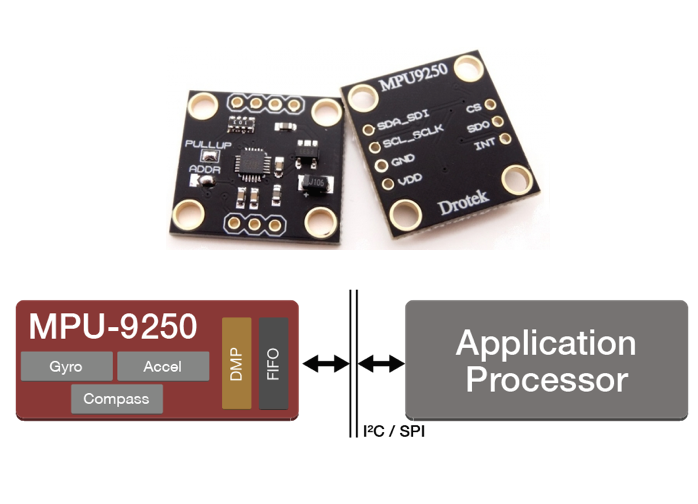
\includegraphics[scale=0.35]{mpu9250.png}
\caption{MPU-9250}
\label{fig:mpu9250}
\end{figure}

The MPU-9250 is a System in Package device (SiP) that combines two chips: the MPU-6500 device (used in the first feasibility study \cite{Santaera:ICRA:2015}) containing a 3-axis gyroscope and a 3-axis accelerometer, and the AK8963, a market leading 3-axis digital compass. In particular:

\begin{itemize}
\item[$\cdot$] \textit{Accelerometer}: Use separate proof masses for each axis. Acceleration along a particular axis induces displacement on the corresponding proof mass, and capacitive sensors detect the displacement differentially. The 3-analog information is digitized using individual on-chip 16-bit Analog-to-Digital Converters (ADCs) to sample each axis;

 \item[$\cdot$] \textit{Gyroscope}: There are three indipendet vibratory rate gyroscopes, wich detect rotation about the X, Y and Z axes. When the gyroscope are rotated about any of sense axes, the Coriolis force causes a vibration that is detected by a capacitive pickoff. The resulting signal is amplified, demodulated and filtered to produce a voltage proportional to the angular rate. This voltage, as for the accelerometer, pass thorugh a ADC providing digital outputs.

 \item[$\cdot$] \textit{Magnetometer}: The 3-axis magnetometer uses higly sensitive Hall sensor technology. It detects a magnetic field in the X, Y and Z axes. As the other, each ADC has 16-bit resolution.
\end{itemize}

\noindent The MPU-9250's technical features are summarized in the Table \ref{tab:mpu}.
\begin{table}[tb]\footnotesize
\caption{MPU-9250 features}
\centering
\label{tab:mpu}
\begin{tabular}{l | c | l}
\textbf{Part} & \textbf{Unit} &  \\ \hline \hline
Gyro Full Scale Range & (deg/sec) &  $\begin{array}{l}   \pm 250 \\  \pm 500  \\ \pm 1000 \\ \pm \textbf{2000} \end{array}$  \\
\rowcolor [gray]{.8}  \text{Gyro Rate Noise} &  (\text{dps}/$\sqrt{\text{Hz}}$)  & $\begin{array}{l}   0.01 \end{array}$  \\
\text{Accel Full Scale Range} & (\text{g}) & $\begin{array}{l}   \pm 2 \\  \pm 4 \\  \pm \textbf{8} \\ \pm 16 \end{array}$ \\
\rowcolor [gray]{.8} \text{Compass Full Scale Range} &($\mu\text{T}$) & $\begin{array}{l}   \pm \textbf{4800} \end{array} $\\
\text{Digital Output} &  & $\begin{array}{l} \text{I}^2\text{C} \\ \textbf{SPI}   \end{array} $ \\
\rowcolor [gray]{.8} \text{Logic Supply Voltage } & (\text{V}) & $\begin{array}{l} 1.7\text{V}\text{to}\text{VDD} \\ \textbf{VDD}   \end{array} $\\
\text{Package Size} & (\text{mm}) & $\begin{array}{l} 3\text{x}3\text{x}1   \end{array}$
\end{tabular}
\end{table}


The output data from  axes sensors can be read,  in digital way, from a 8-bit  register of the device.  Each axis sensor presents two registers: the  up  and the low register. Thus, a complete information from a specific sensor occupies 48-bit.  Considering, for example, the accelerometer there are 16-bit for the x axis, 16-bit for the y axis and 16-bit for the z axis.

Figure~\ref{fig:axes} shows the orientation of the axes of sensitivity and the polarity of rotation.
\begin{figure}[h]
\centering
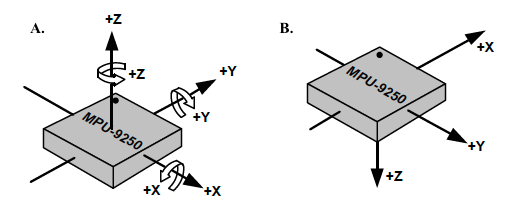
\includegraphics[scale=0.5]{axes_orientation.png}
\caption{A. accelerometer and gyro orientation axes  B. magnetometer oreintation axes}
\label{fig:axes}
\end{figure}

As already mentioned, a complete sensorization of the glove and, therefore, of the hand needs 17 IMUs. This means that for keeping the time response of the system low, the communication between a master processing unit and each IMU becomes a crucial aspect. The MPU-9250 supports two different types of digital communication: I$^2$C (Inter Integreted Circuit) and SPI (Serial Peripheral Interface). The I$^2$C maximum working frequency is 400Hz, while the SPI works on 1Mhz. Therefore, the SPI allows a faster communication and using the a further pin (Slave-Select pin) allows the user to use a single bus overcoming to the problem of set an unique address for each sensor.

In Figure~\ref{fig:spi}, the pin-out of a generic SPI communication is shown. In particular, the SPI is a 4-wire synchronous serial interface that uses two control lines and two data lines:
\begin{itemize}
\item[-] SCLK, clock - control line;
\item[-] MOSI, master-output slave-input - data line;
\item[-] MISO, master-input slave-output - data line;
\item[-] SS,   slave select - control line.
\end{itemize}

\begin{figure}[h]
\centering
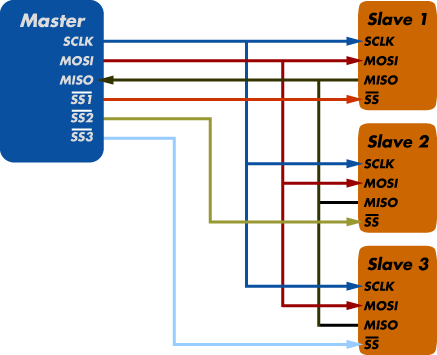
\includegraphics[scale=0.4]{spi.png}
\caption{Scheme of SPI communication}
\label{fig:spi}
\end{figure}

In our work, the MPU-9250 always operates as a Slave device during standard Master-Slave SPI operation. To speed up communication between master and sensors, in our work three SPI bus are used (\ref{fig:firmwarepage1}, \ref{fig:IMU_Glove_bus}).  In each bus the SCLK, the MISO and the MOSI pin are shared by all slaves devices, while each slave devices requires its own SS line to communicate with the master. The SS pin goes low, (\textit{active}) when the transmission start, and comes back high (\textit{inactive}) at the end, so only one SS line is active at a time, ensuring that only one slave is selected at any given time.

\begin{figure}[h]
\centering
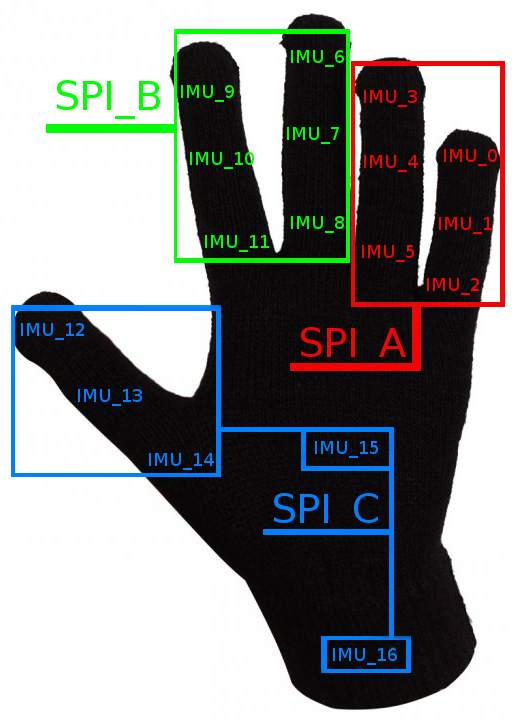
\includegraphics[scale=0.4]{Glove_IMU_SPI.png}
\caption{SPI bus used in the IMU Glove}
\label{fig:IMU_Glove_bus}
\end{figure}

Usually the master is a microcontroller  or any processing unit that support SPI communication. To manage all 17 slave devices,  a microcontroller with a sufficient number of pins is needed. The microcontroller must be able not only to read the correct data from the IMUs but also it must be able to send  data packages to the PC, where the Magdwick Filter is implemented.   \\
\newline

\subparagraph{PSoC 5LP}

The processing unit used is a PSoC mounted on the \textit{PSoC 5LP} board developed by Cypress Semiconductor \cite{PSOC5LP}. The PSoC is a low power ARM \textsuperscript \textregistered Cortex - M3 based programmable system on chip devices offering unmatched high-precision analog and the flexibility to design custom system solutions. Combined with the free PSoC software development tools (PSoC Creator and
PSoC Programmer) from Cypress, this board is a good solution for applications who need different hardware devices and good time response. %in able to offer a large range of internal devices and solutions necessary to our application.

%more than sufficient for creating anything from basic microcontroller with embedded analog and digital functions to a highly complex system controller. Both the hardware system architecture and the software are supported by the PSoC
%software tools.
The PSoC integrated circuit is composed of a core, configurable analog and digital blocks, and programmable routing and interconnect. The configurable blocks in a PSoC are the biggest difference from other microcontrollers: for this reason it can be associated to the FPGA microcontroller family (Field-Programmable Gate Array).
%\begin{figure}[h]
%\centering
%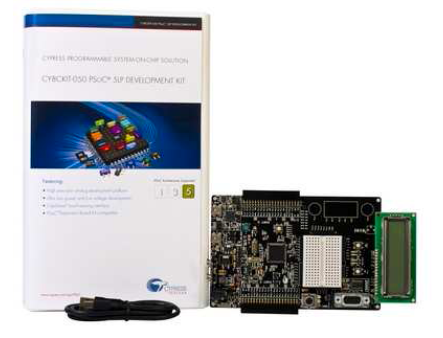
\includegraphics[scale=0.5]{psoc.png}
%\caption{PSoC 5LP}
%\label{fig:psoc}
%\end{figure}

By using configurable analog and digital blocks, it is possible to  create and change mixed-signal embedded applications. These blocks are designed by PSoC-Creator, an Integreted Design Environment (IDE).
%The development of the PSoC 5LP  and PSoC-Creator has permitted to managed  the IMUs easily.
%In our work the PSoC is used first to communicare with IMU then to send data read from sensors to computer.

The first task of the microcontroller is to read data from the slave devices allowing a SPI communication. The SPI bus could be only one, but three separated bus were preferred to have greater control on the hardware system and to speed up the communication.
\begin{figure}[h]
\centering
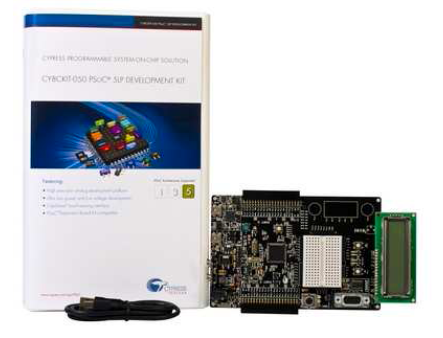
\includegraphics[scale=0.5]{psoc.png}
\caption{SPI buses on the IMU glove}
\label{fig:spibuses}
\end{figure}

After all IMU data are read, the data are stored in the EEPROM of the PSoC5 and are ready to be send to the PC. To communicate with the PC, the PSoC5 has a dual-channel USB. A first channel \textit{A} %of the highspeed USB interface is
is connected to the PSoC 5 in FIFO parallel mode to allow a fastest transfers between the USB host PC and the PSoC 5. A second channel \textit{B} is connected to the PSoC 5 in serial mode to allow a standard UART communication between the host PC and the PSoC5. However, channel A, commonly used to implement fast a communication, has a little communication buffer composed by 64 byte, while to send all IMU data to PC we need more than 450 bytes. The channel B is instead a serial RS-232 channel and needs a Serial-USB converter to be connected to the PC. The PSoC 5LP mount on board presents an internal Serial-USB converter but its maximum speed is 115200 baud while we need more than 900000 baud.
Starting from these considerations, a different solution was implemented using on PSoC a standard serial communication and an external Serial-USB module to connected PSoC board to PC.

\subparagraph{Serial Communication}

The communication between PSocC5 and PC was created exploiting the serial adapter 990 004 \cite{Serial_USB}. It is optimum to connect microcontroller and logic circuit to a PC with an high rate trasfer data. The heart of the module is the chip FT232R distributed by FTDI \cite{FDTI_homepage} which works with a supply tension of 3.3V, thus it possible to connect the device to another TTL peripheral o microcontroller in the range of 3.3V-5V without the problem to convert the signal RS232 to  the TTL. The size of the circuit are very small, 25x18 mm and
\begin{figure}[h]
\centering
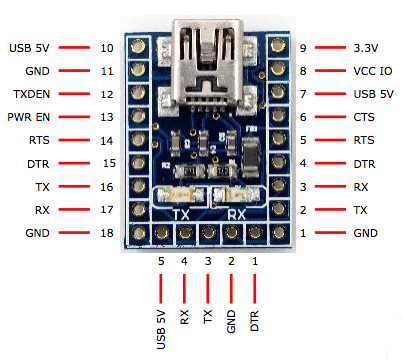
\includegraphics[scale=0.3]{usb_serial.png}
\caption{Serial adapter}
\label{fig:serial_adapter}
\end{figure}
two led visualize input-output data of serial port, very useful to control data stream, avoiding possible software/hardware problems. The device is USB 2.0 compatible and it allows full speed of 1Mb.

\begin{figure}[h]
\centering
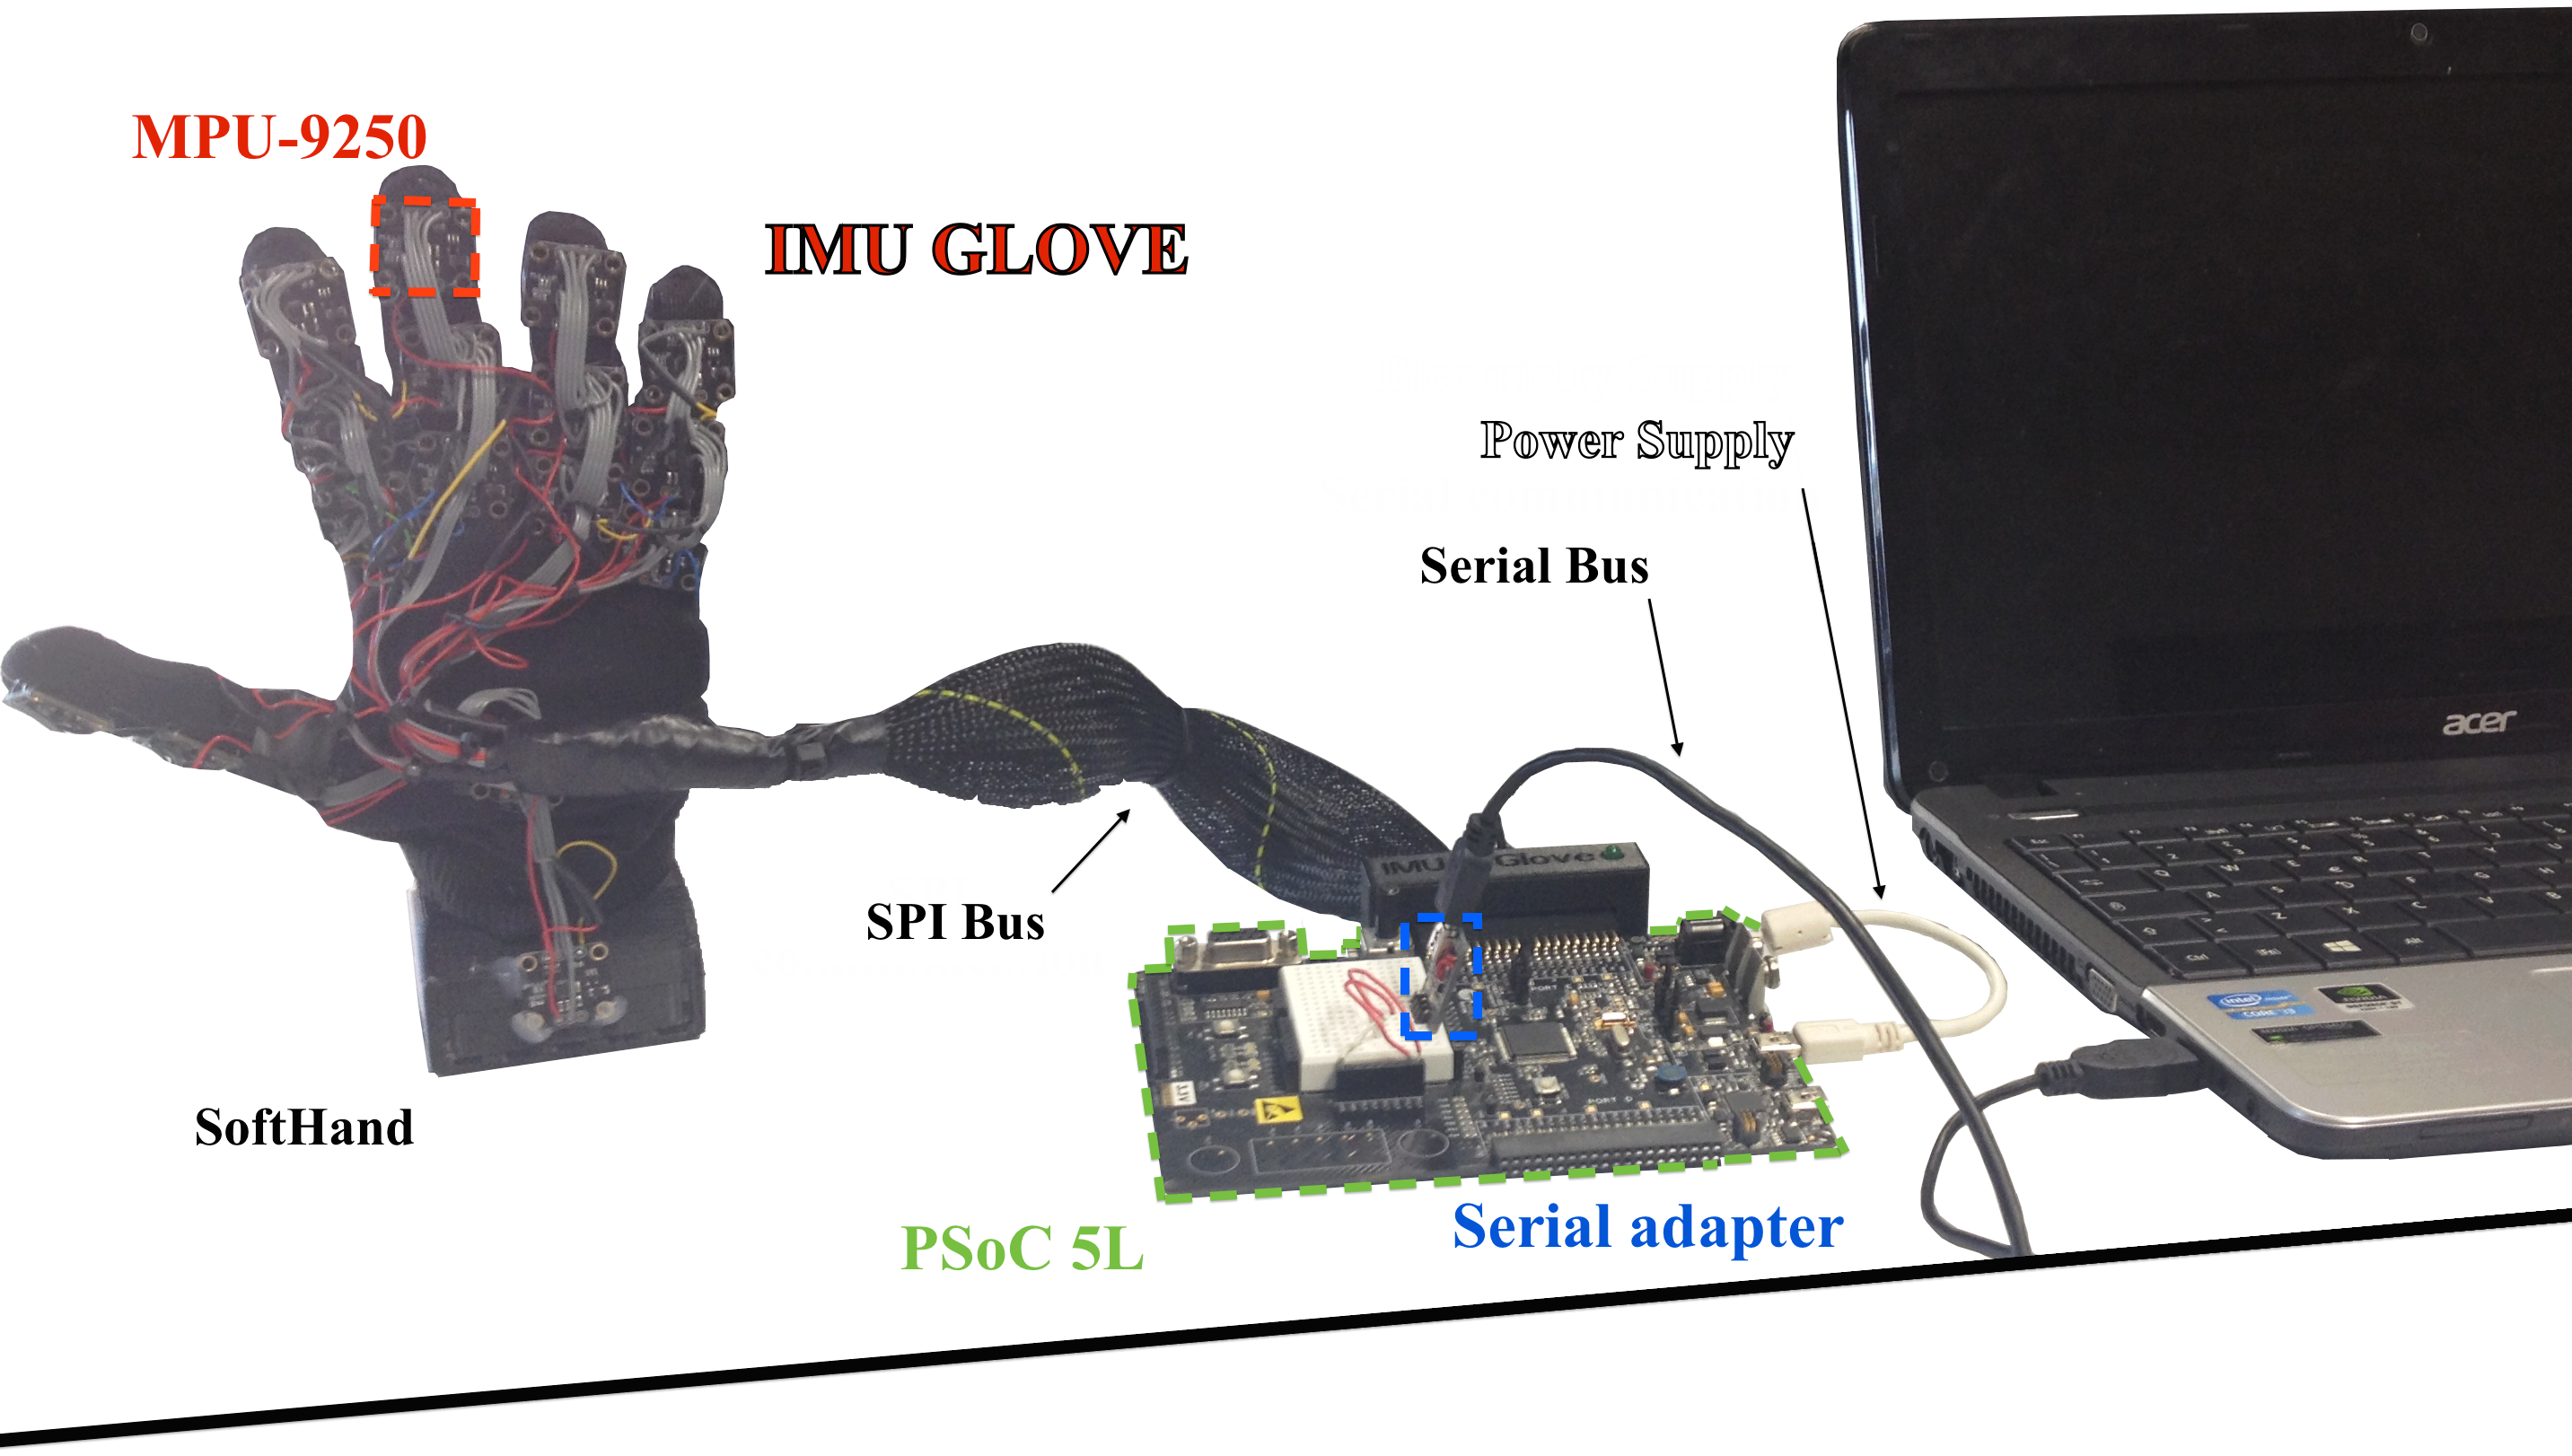
\includegraphics[scale=0.125]{hardware.png}
\caption{Full Hardware}
\label{fig:hardware}
\end{figure}


\paragraph{(c) Software}

To reconstruct the hand complete posture using the IMU glove two different software are written. The first one, written in C, running on the PSoC is its firmware and this one as described read all IMU measurements and then send data to a PC.
The second software, written in C++, running on a PC reads data from PSoC and applies in a suitable way the Madgwick filter to data from two subsequent IMU.
%The hardware described was managed in two fundamental step.  From one side there was the necessity to read IMU data and send its to computer, from the other side the sensor informations must be used to implement the algorithm for the  hand posture reconstruction.
%This was possible exploiting the PSoC5L where the \textit{Firmware} was installed and the \textit{Software} written in C++ in a Personal-Computer.

\subparagraph{Firmware on PSoC}

The firmware is written using the PSoC creator IDE developed by Cypress. This one offers an intuitive GUI to
%First of all the SPI communication was created between PSoC5L and the IMUs via software, where the PSoC5L  was the master and the IMUs the salves.  This was possible exploiting PSoC Creator, the software developed by Cypress. It
manage the internal PSoC devices represented as code blocks, to configure the PSoC input/output, and to write the code necessary to connect and work PSoC internal device and pin. % so all necessary pins of the PSoC's board were configured take advantage of the GUI offers by the IDE.
Figure~\ref{fig:firmwarepage1} shows how the three SPI bus are configurated and the relative pin used.%How the SPI communication was implemented is possible to view in the figure

\begin{figure}[h]
\centering
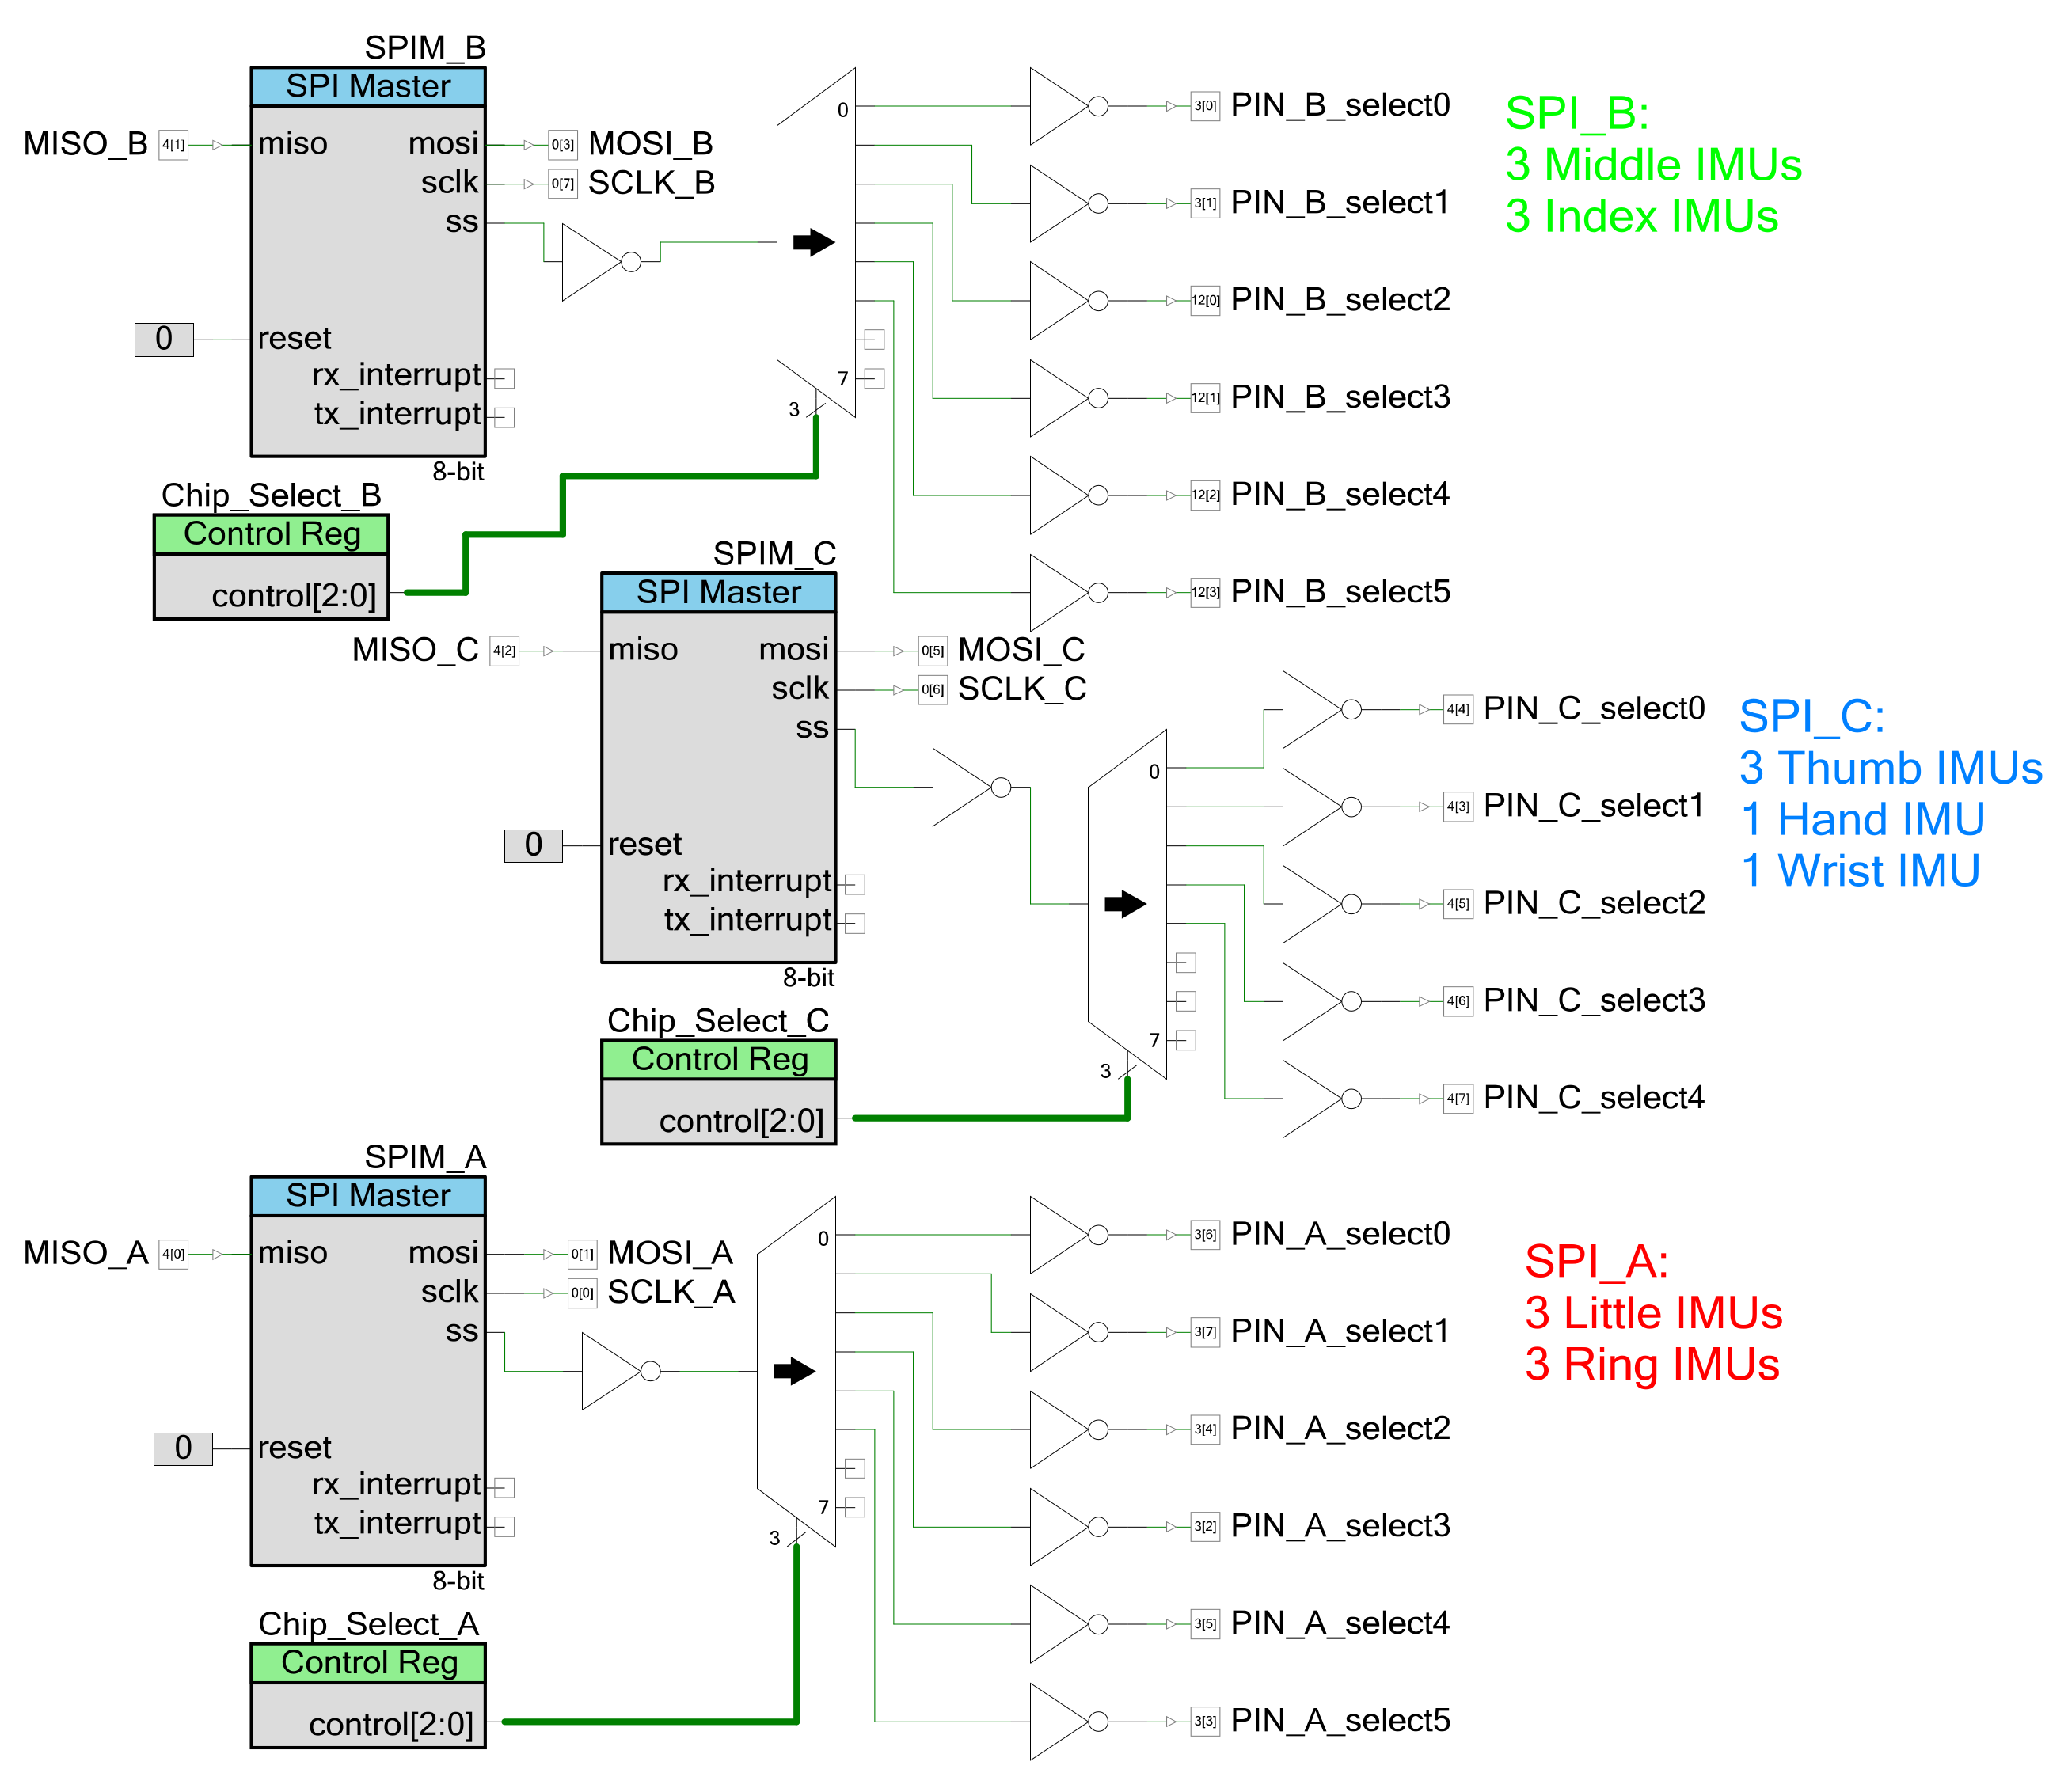
\includegraphics[scale=0.7]{Fimware_Page1.png}
\caption{SPI blocks in the IDE}
\label{fig:firmwarepage1}
\end{figure}

Figure~\ref{fig:psocfirmware} shows how the firmware manages the IMUs. %Guaranteed the communication between the sensor and the PSoc5L,  the firmware was written in the memory of the board, figure \ref{fig:psocfirmware}.
\begin{figure}[h]
\centering
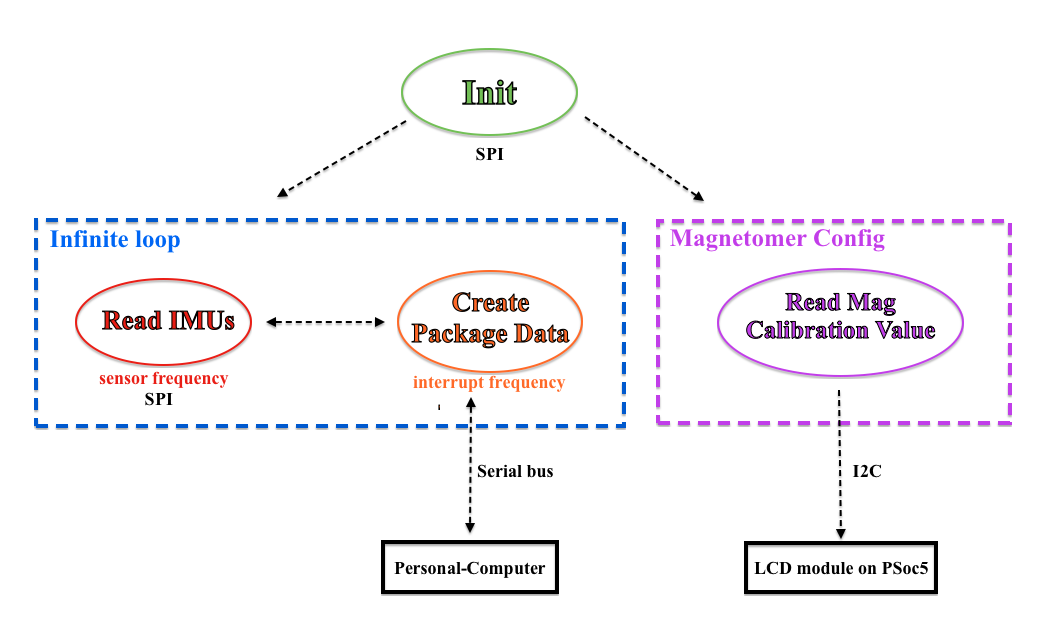
\includegraphics[scale=0.35]{firmware.png}
\caption{Scheme of Firmaware written in the PSoC5L}
\label{fig:psocfirmware}
\end{figure}
In particular, there is an initalization phase \textit{Init}, where all IMU internal registers are set. This means configure, e.g. internal clock, type of communication, accelerometer, gyro full scale range, etc.
After the initialization phase firmware could run in two different ways. The \textit{Magnetometer Config}, performed whenever there are new IMUs, helps to know sensitivity adjustment data for each magnetometer axis. In fact, due to constructive inaccuracies during the magnetometer installation on the MEMS, the magnetometer axis pose or orientation can be different between two IMUs. Therefore, the manufacturer stores in each IMU 8-bit register, three numbers (one for each axis), to equalize magnetic measurements between two o more IMU. In particular, these registers are:

\begin{enumerate}
\item[$\cdot$] $ASA_x[7:0]$: Magnetic sensor X-axis sensitivity adjustment value
\item[$\cdot$] $ASA_y[7:0]$: Magnetic sensor Y-axis sensitivity adjustment value
\item[$\cdot$] $ASA_z[7:0]$: Magnetic sensor Z-axis sensitivity adjustment value
\end{enumerate}

Read the three sensivity registers the sensitivity factor corrector $s_a$ is given by %adjustment is done by the equation below

\begin{equation}
s_a  = \frac{ 0.5(ASA_a - 128)}{128} + 1,
\end{equation}

\noindent and for example the exact magnetic field on the $x$-axes is given

\begin{equation}
H_{{adj}_x} = H_x s_x,
\end{equation}

\noindent where $H_x$ is the current data read from the measurement data register, $ASA_x$ is the sensitivity $x$-axes correction factor and $H_{{adj}_x}$ is the real measurement.
%To Each values is possible to view on the LCD module on the PsoC's board via I2C.
After the all magnetometer correction factors are computed, these ones are store on the PC hard disk and then are used to correct the current data read from PSoC. %The magnetometer config step runs only one time, because  the adjustment parameters, once known, are stored by the user in the C++ code in the Personal-Computer.

If all magnetometer corrector factors have been computed after the initialization phase, firmware will run \textit{Infinite loop} phase. This is subdivided in two independent sections
\begin{enumerate}
\item[$\cdot$] \textit{Read IMUs}: An internal counter each $20$ms (50Hz) generates an interrupt where IMU are sequentially read and the output data stored in 3 different matrices
                          \begin{enumerate}
                          \item[-] Acc $\in \Re ^{17 \text{x} 3}$
                          \item[-] Gyro $\in \Re ^{17 \text{x} 3}$
                          \item[-] Mag $\in \Re ^{17 \text{x} 3}$
                          \end{enumerate}
                          The maximum read frequency is the lowest one among the three sensors, and in particular the magnetomer has the lowest refresh frequency 100Hz.
\item[$\cdot$] \textit{Create Package Data}:  Between two subsequent interrupt data stored in the three matrices are reorganized in a package ready to be sent to the PC. The package  is summarized in Figure~\ref{fig:package}
\begin{figure}[h]
\centering
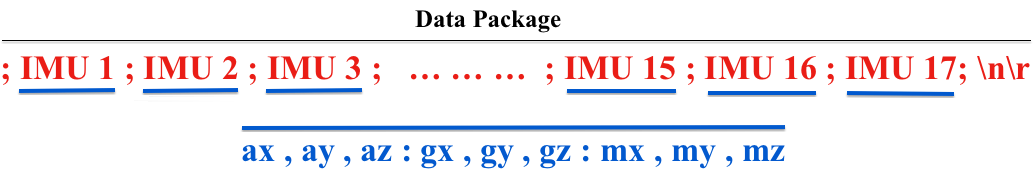
\includegraphics[scale=0.3]{datapackage.png}
\caption{Data package sent to  the PC}
\label{fig:package}
\end{figure}

\noindent where its length is
\begin{equation*}
\displaystyle  \left. \begin{array}{lccc}
\text{int} & \text{ax},\quad \cdots, \quad \text{mz}  & = & 2 \text{byte} \\
\text{char} & , & = & 1 \text{byte} \\
\text{char} & : & = & 1 \text{byte} \\
\text{char} & ; & = & 1 \text{byte} \\
\text{char} & \backslash \text{r} & = & 1 \text{byte} \\
\text{char} & \backslash \text{n} & = & 1 \text{byte}
\end{array} \right\rbrace \;
\begin{array}{lcl}
\textcolor{blue}{\text{int}} \; = \; 9 \; \cdot \; 17 \; & = & 306 \; \text{byte} \\
\textcolor{blue}{\text{char}} \; = \; 8  \; \cdot \;+\; \; \textcolor{red}{\text{char}} \; \cdot \; 20  & = & 156 \; \text{byte}  \\
& & \\ \hline
 & & \text{462 byte}
\end{array}
\end{equation*}

\noindent The interrupt that defines the IMU read and data send time is generated using an PWM block, while the communication with the computer is implemented using an UART block, as shown in Figure~\ref{fig:firmwarepage1}

%The sent of this package is regulated by an interrupt every 50Hz via Serial bus.  The serial bus is managed developing PSoC Creator too. The frequency of interrupt is created by PWM block while for the serial communication a UART block is implemented, figure \ref{fig:firmwarepage1}.

\begin{figure}[h]
\centering
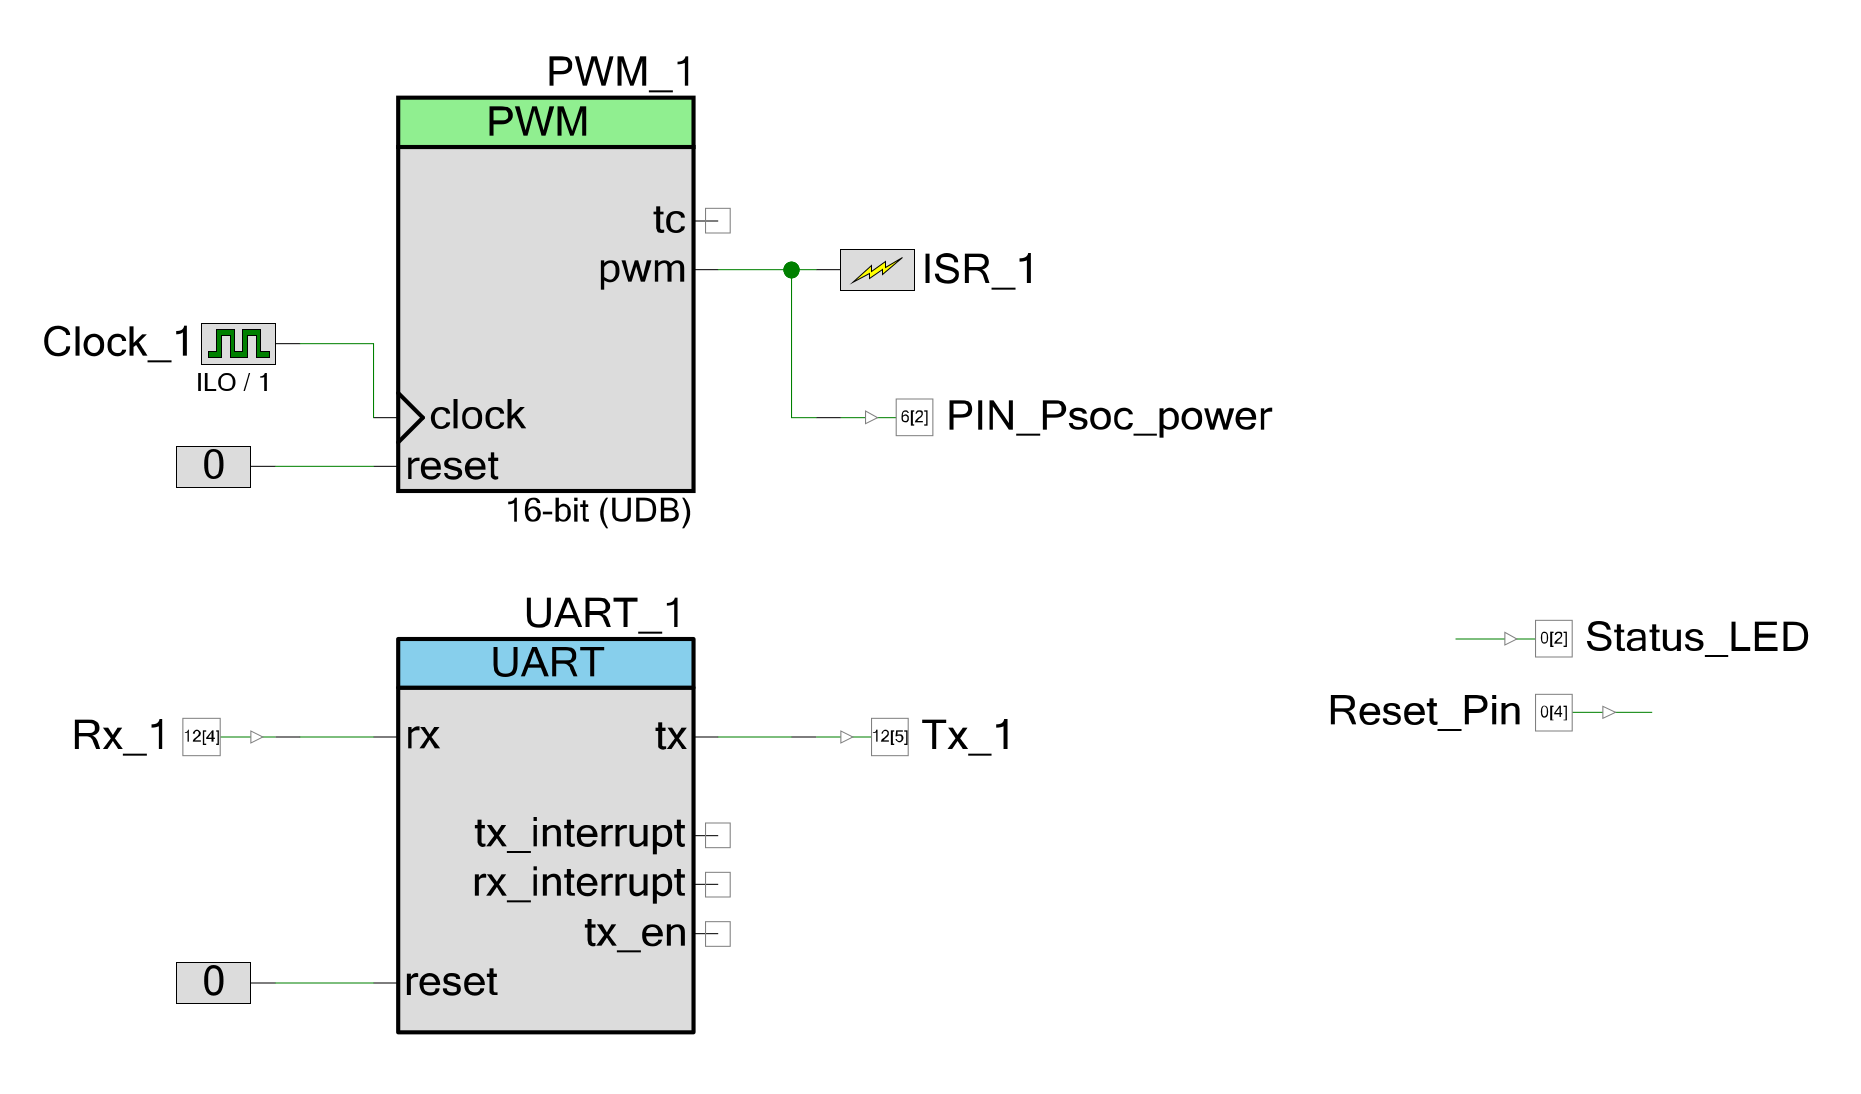
\includegraphics[scale=0.8]{Fimware_Page2.png}
\caption{Interrupt and UART blocks in the IDE}
\label{fig:firmwarepage1}
\end{figure}
\end{enumerate}

\subparagraph{C++ code on PC}
The code on PC implements, from data read by PSoC, the Madgwick algorithm between two IMUs. A scheme of the code is shown in Figure~\ref{fig:code_c}.

\begin{figure}[h]
\centering
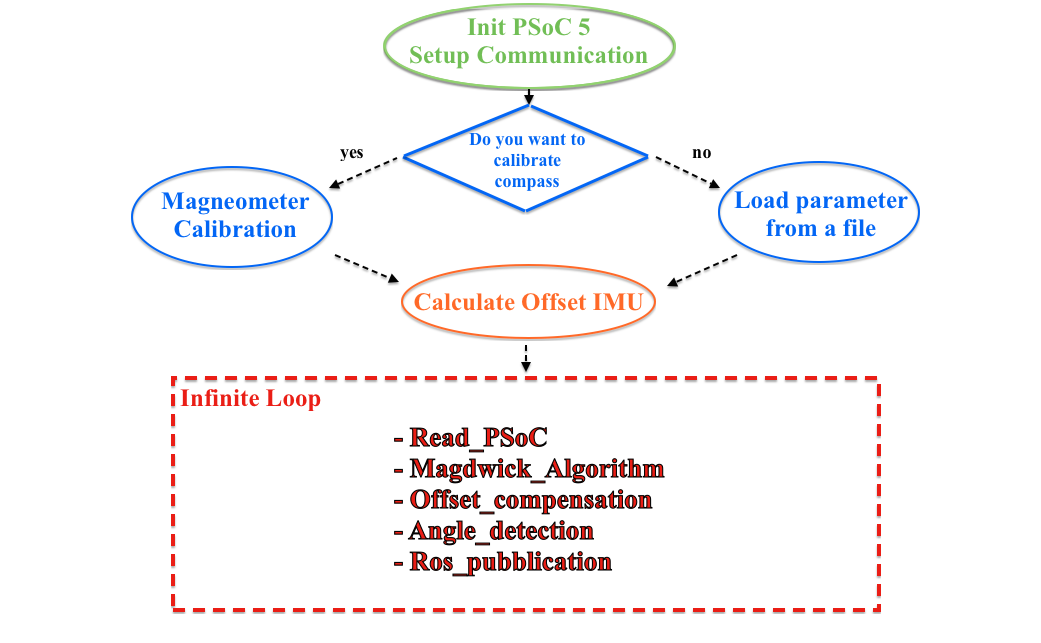
\includegraphics[scale=0.35]{code_c.png}
\caption{Code C++ implemented in the PC}
\label{fig:code_c}
\end{figure}

During an initial phase, the communication with the PSoC is configured, then the user can decide whether to change or not the magnetometer calibration factors. If the user decides to change the magnetometer calibration factors, a special function
to calibrate correctly magnetometer will run, and the new compass correction parameter will be stored in a file.txt to be load in the future. Magnetometer calibration takes about 50-60 seconds to compute all magnetometer correction factors.
If the user decides to keep the previous magnetometer corrector factors, software applies the Madgwick filter to data read from the IMU to compute the offset angles between IMUs due to glove mounting inaccuracies. Then, after these initial stages, software enters in a infinite loop where it keeps computing, at each time instant, the joint angles values from the current IMU measurements.

Once the offset quaternion is detected, the infinite loop starts calculating the desired joint angles.

\paragraph{(d) Validation}

In order to validate the hand posture reconstructed using the IMU glove, and to demonstrate the ability for a robot to recognize a grasped object from the knowledge of its hand posture, some simple experiments have been performed.
To validate the hand posture, a Pisa/IIT SoftHand is dressed with the IMU glove. On line visualization of the hand posture is programmed wth ROS (Robot Operating System) \cite{Ros_homepage}. Figs. \ref{fig:hand_reconstruction_1}, \ref{fig:hand_reconstruction_2} and \ref{fig:hand_reconstruction_3} show three different examples of hand posture reconstruction, while the two videos show the hand posture reconstruction, respectively, in \href{https://www.youtube.com/watch?v=0oVha0Q1vWM}{static} and \href{https://www.youtube.com/watch?v=bceOXa990-Q}{dynamic} case.

\begin{figure}[h]
\centering
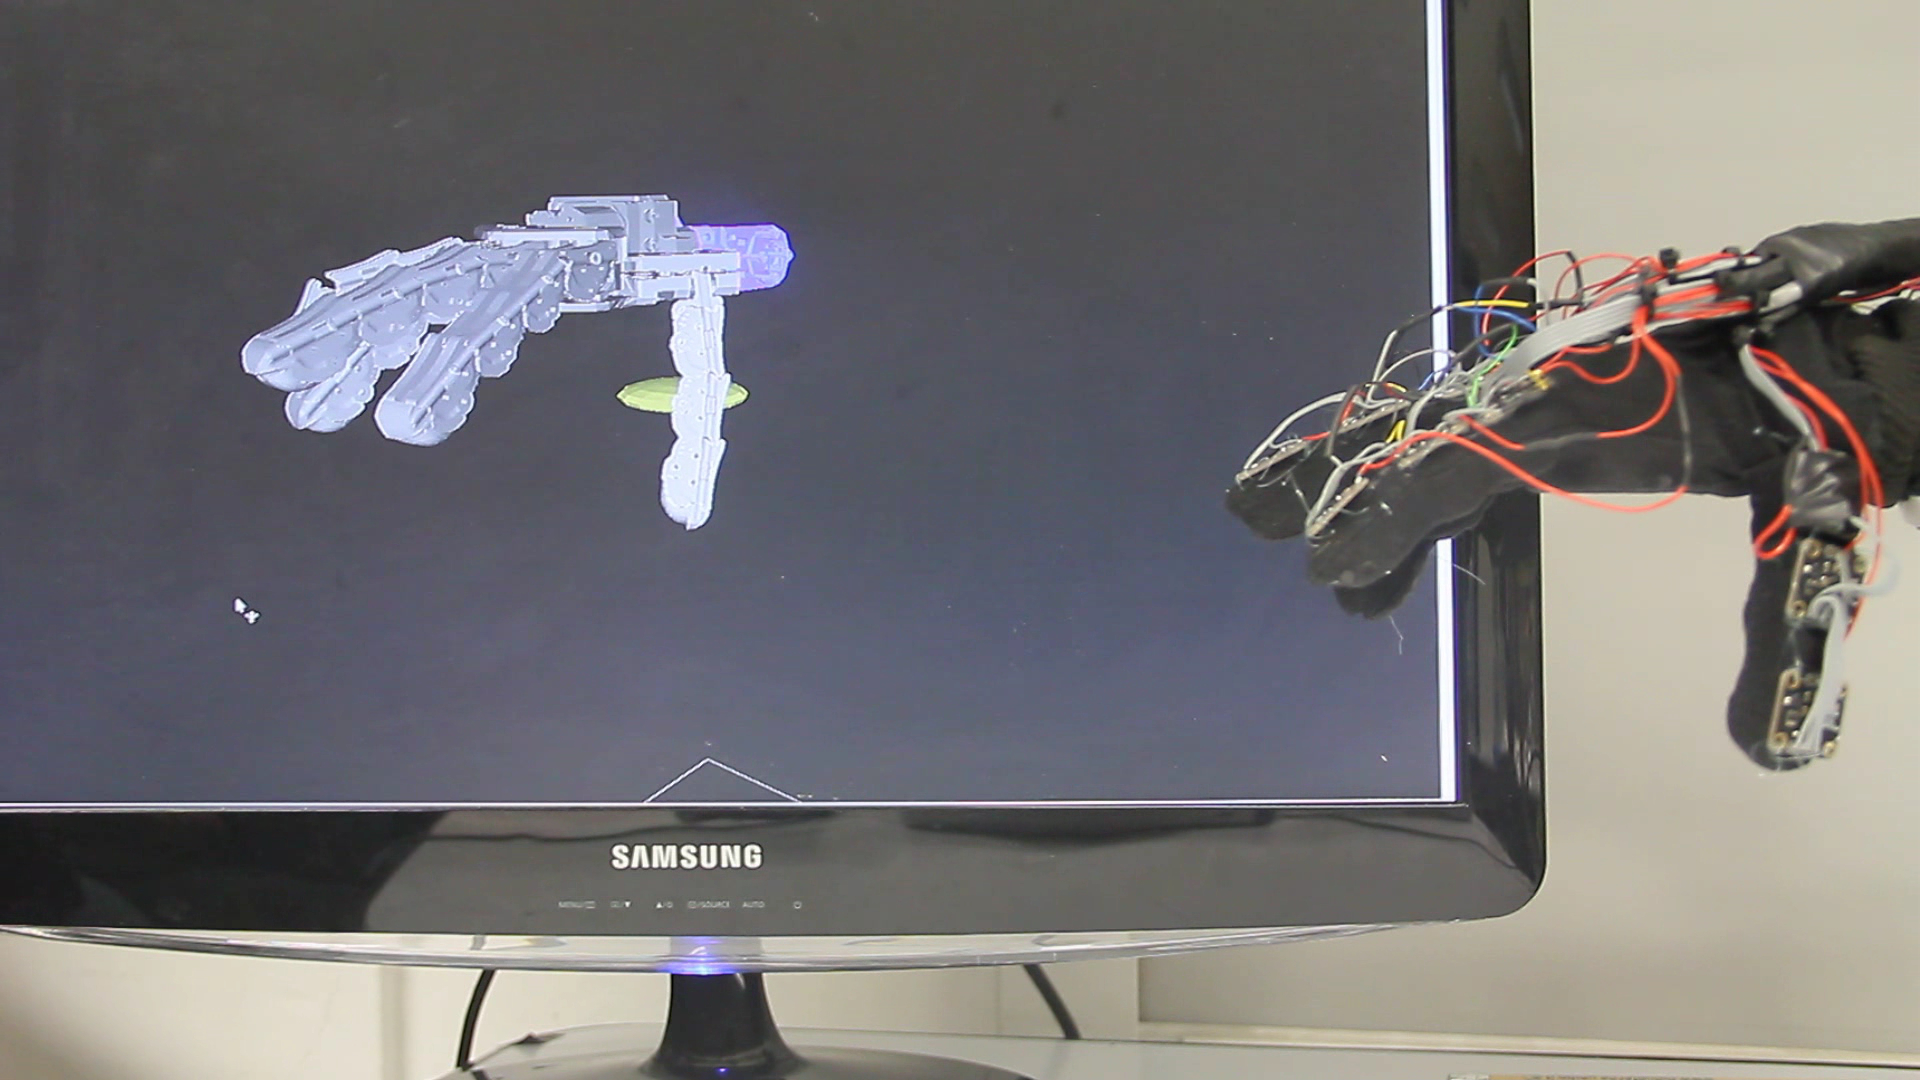
\includegraphics[scale=0.20]{Hand_Movement_1.png}
\caption{Hand Posture Reconstruction Example}
\label{fig:hand_reconstruction_1}
\end{figure}

\begin{figure}[h]
\centering
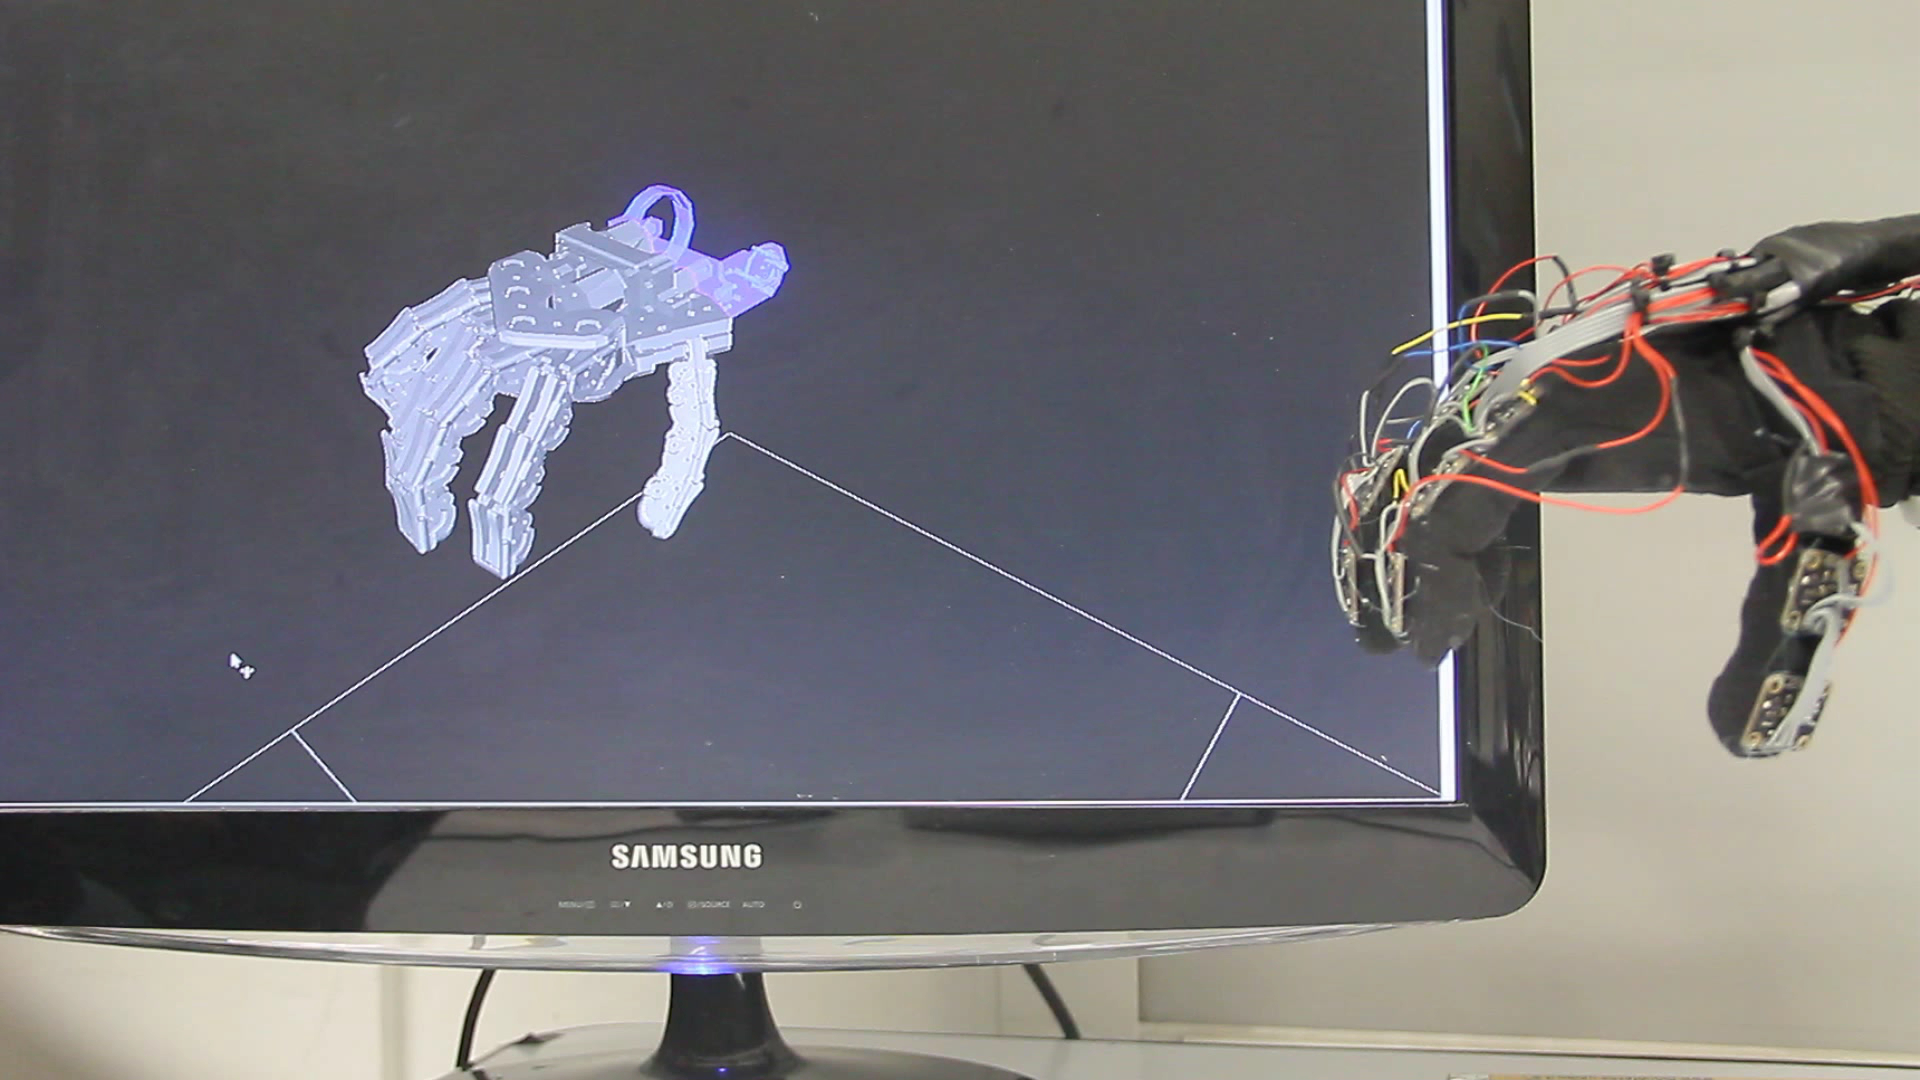
\includegraphics[scale=0.20]{Hand_Movement_2.png}
\caption{Hand Posture Reconstruction Example}
\label{fig:hand_reconstruction_2}
\end{figure}

\begin{figure}[h]
\centering
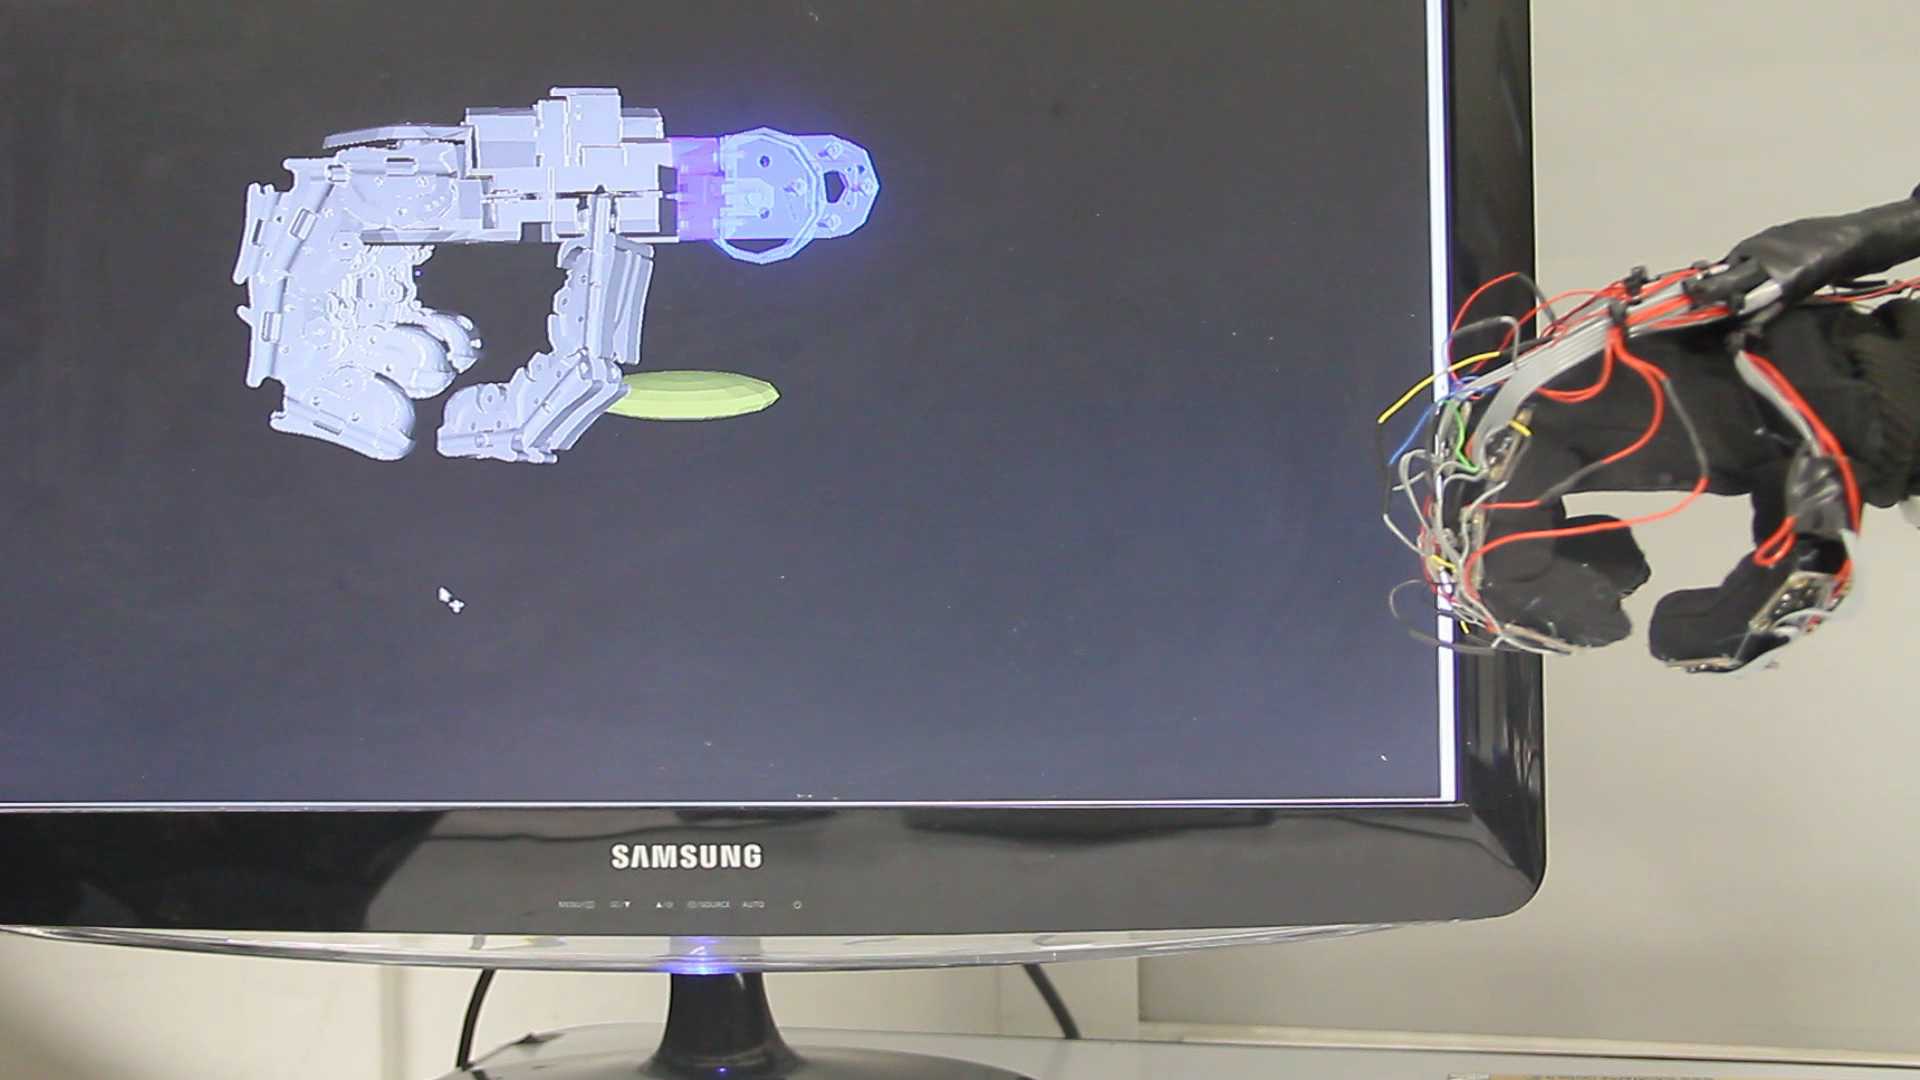
\includegraphics[scale=0.20]{Hand_Movement_3.png}
\caption{Hand Posture Reconstruction Example}
\label{fig:hand_reconstruction_3}
\end{figure}

To study the ability of a robot to recognize a grasped object knowing the posture of its hand, a set of five cups are used. Four of the five cups come from the PaCMan object database. All cups have different diameters as shown in Table~\ref{tab:cups}.

\begin{table}[tb]\footnotesize
\begin{tabular}{cc} \hline \hline
Cups Number & Diamter \\ \hline
\#1 & 55mm \\
\#2 & 76mm \\
\#3 & 82mm \\
\#4 & 90mm \\
\#5 & 98mm.
\end{tabular}
\caption{Probed Cups}
\label{tab:cups}
\end{table}

The object recognition experiments is composed by two different steps: \textit{Learn} and \textit{Recognize}. During the two phases the hand is used as a probe.
The hand movements (open/close) are managed by a simple PID controller. In this first phase, the $K_p$, $K_d$ and $K_i$ parameters of the PID controller are set to values such that the hand squeezing force is kept low. In these conditions, the hand is not able to grasp an object, but behaves as a probe.

In the learning phase, when the hand probes an object, the software running on the PC appends in a matrix format  (saved in a text file) a twenty elements row. This row is composed by a first number which identifies the object and by other nineteen elements which report the current joint angles values (4 for little, 4 for ring, 4 for middle, 4 index and 3 for thumb).

In the recognition phase, the software reads the text file where the learning data are saved and creates a matrix $O_{bj} \in \mathbb{R}^{n \times 20}$, where $n$ is the number of learned objects.
Then, the hand in closing, probes the current object and software compares the current joint angles values with the values recorded during the learning phase.

To start off to match the joint angles values, a brute force root mean squares error minimizer was considered. Here, the software returns $n$ different numbers $m_n$ representing the distance of each of the $n$ hand recorded poses to the current hand pose. Trivially, the object in database whose hand pose signature is  closest to the current one, has the smallest $m_n$ number.
For each learned object, $m_n$ is given by

\begin{equation}
m_n = \sqrt{(C_{angle_{1}} - O_{n_{angle_{1}}})^2 + \cdots + (C_{angle_{19}} - O_{n_{angle_{19}}})^2 },
\end{equation}

\noindent where $C_{angle_{k}}$ is the $k^{th}$ hand current joint angles value, $O_{n_{angle_{k}}}$ is the $k^{th}$ joint angles value of the object $n$ and $k=1, 2 , \cdots , 19$.

With a large number of learned object ($n$) this object recognition strategy could require a large time to match current joints angles values with values recorded in the object database. In future work, we will investigate more efficient strategies (with respect to the current brute force search) to quickly match the current joint angles values with the recorded ones, and to being able to increase object database data types considering, for example, also grasping forces as features.

Figs. \ref{fig:Object_1}, \ref{fig:Object_3} and \ref{fig:Object_5} show three different examples of objects recognition, while the videos show objects recognition procedure respectively for the \href{https://www.youtube.com/watch?v=d_WPQ3WmHRg}{Object 1}, \href{https://www.youtube.com/watch?v=PG38VObdl6o}{Object 2}, \href{https://www.youtube.com/watch?v=bIYhLXm90hc}{Object $3_a$}, \href{https://www.youtube.com/watch?v=IXVlBAoGKho}{Object $3_b$}, \href{https://www.youtube.com/watch?v=Efmm6-JHcxU}{Object $4_a$}, \href{https://www.youtube.com/watch?v=NZElSV_AnJ4}{Object $4_b$}, \href{https://www.youtube.com/watch?v=mDDb5oTaHzM}{Object $5_a$} and \href{https://www.youtube.com/watch?v=sLzU39zffFY}{Object $5_b$}, where the subscripts $_a$ or $_b$ denote if the hand probes the cup handle or no, in this case the cup is recorded as two different objects.

\begin{figure}[h]
\centering
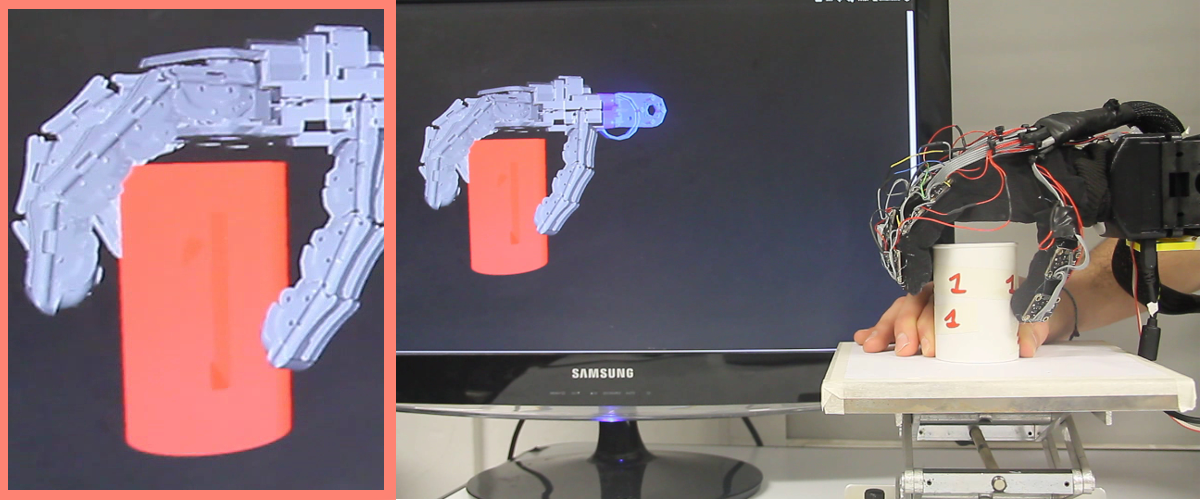
\includegraphics[scale=0.30]{Object_1.png}
\caption{Object Recognition Example}
\label{fig:Object_1}
\end{figure}

\begin{figure}[h]
\centering
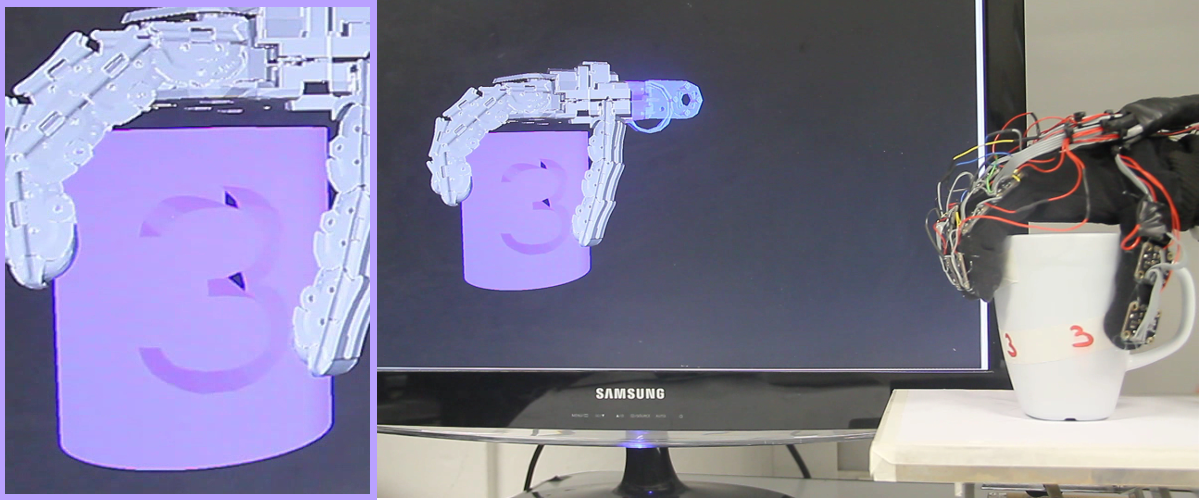
\includegraphics[scale=0.30]{Object_3.png}
\caption{Object Recognition Example}
\label{fig:Object_3}
\end{figure}

\begin{figure}[h]
\centering
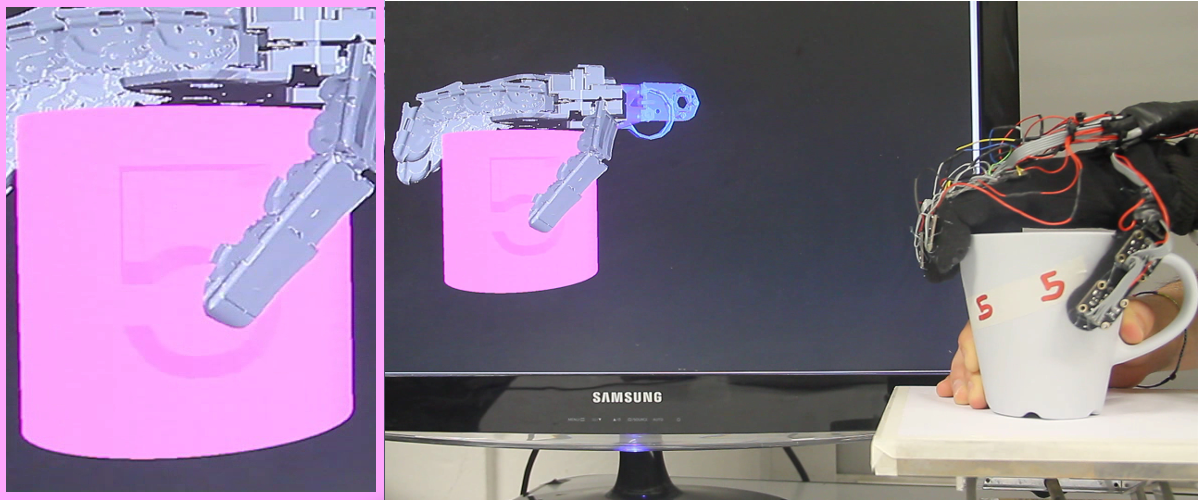
\includegraphics[scale=0.30]{Object_5.png}
\caption{Object Recognition Example}
\label{fig:Object_5}
\end{figure}

\paragraph{Endowing the Pisa/IIT SoftHand with the sense of touch}

We successfully extended the proposed solution above to the case of the five-finger Pisa/IIT SoftHand. We validated the approach by visual inspection as shown in Fig.~\ref{fig:hand_reconstruction_1}. Additional, we suggest watching the video sequences for static \href{https://www.youtube.com/watch?v=0oVha0Q1vWM}{static} and a \href{https://www.youtube.com/watch?v=bceOXa990-Q}{dynamic} configurations\footnotetext{External links are readily identified in the PDF and might not be visible in a black\&white hard-copy, please, click on the PDF to go to the on-line site.}.

\begin{figure}
\centering
\mbox{
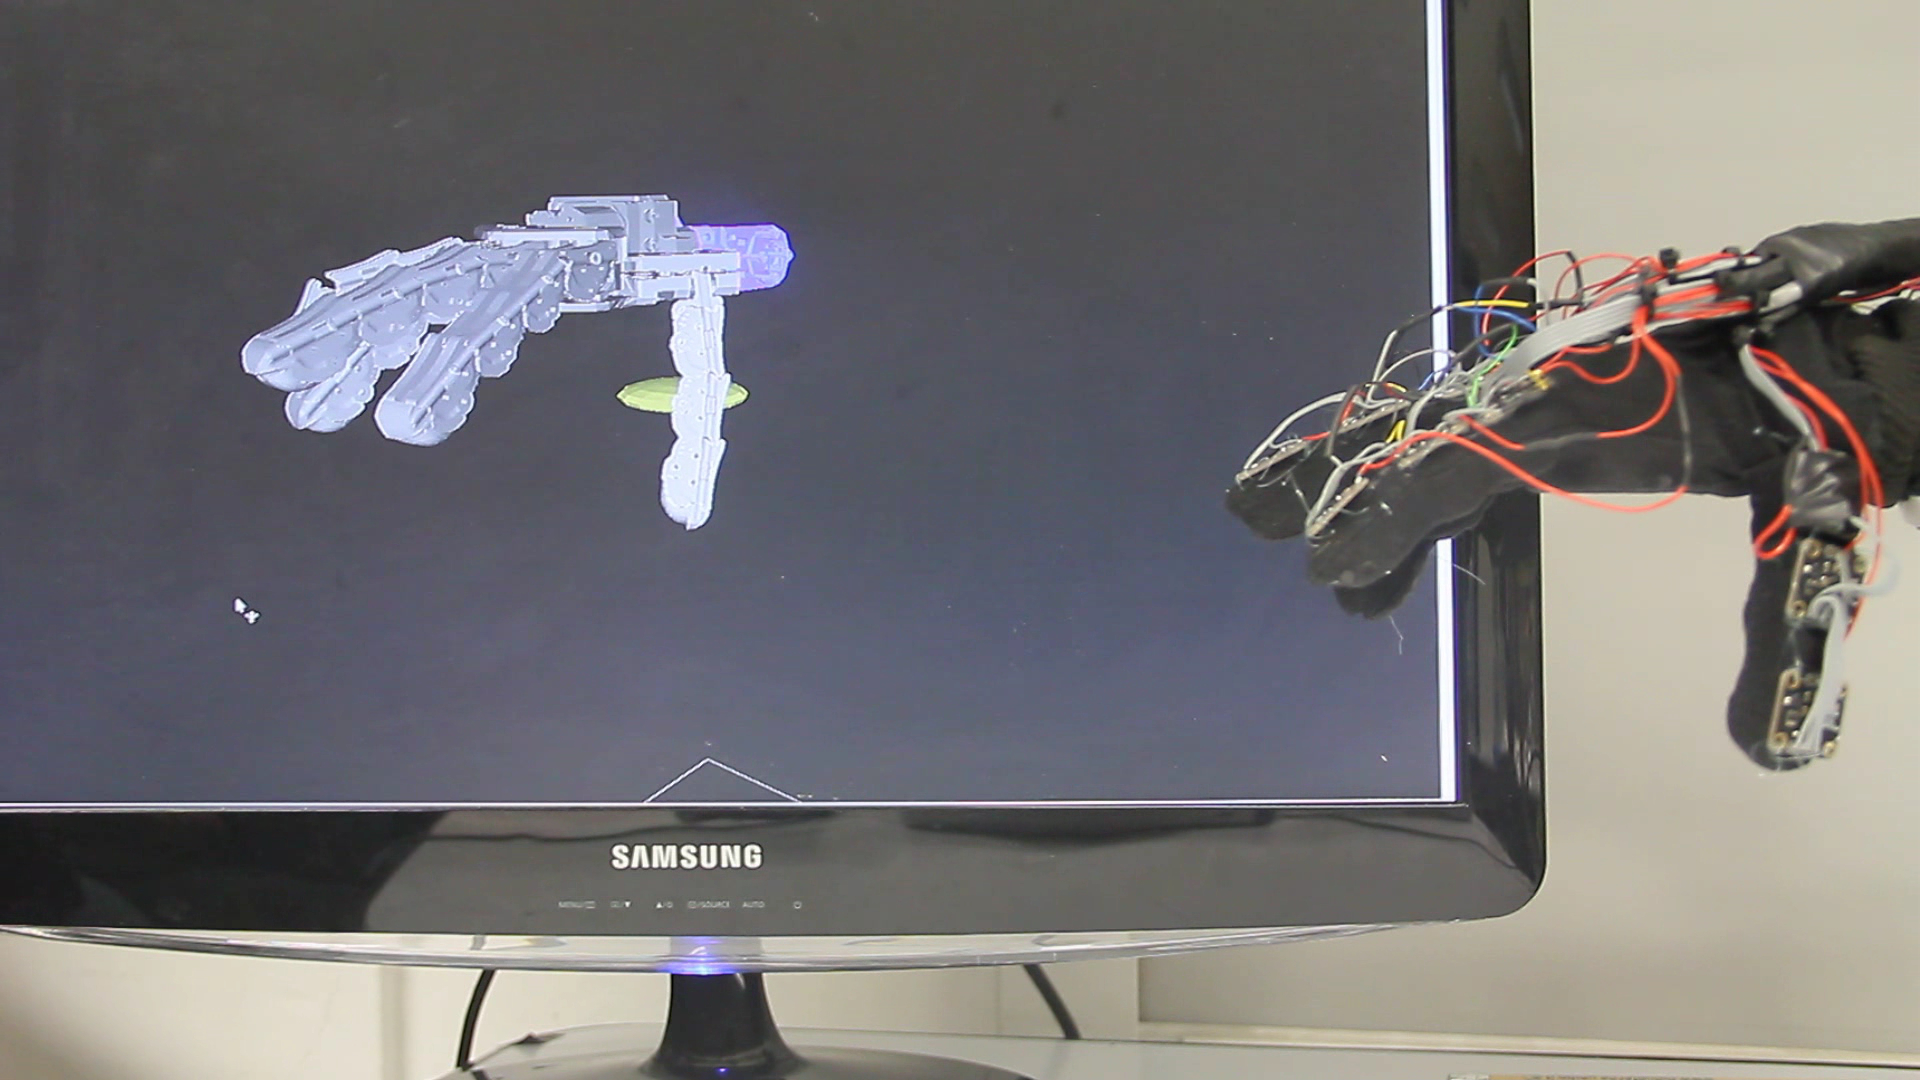
\includegraphics[width=0.33\linewidth]{Hand_Movement_1.png}
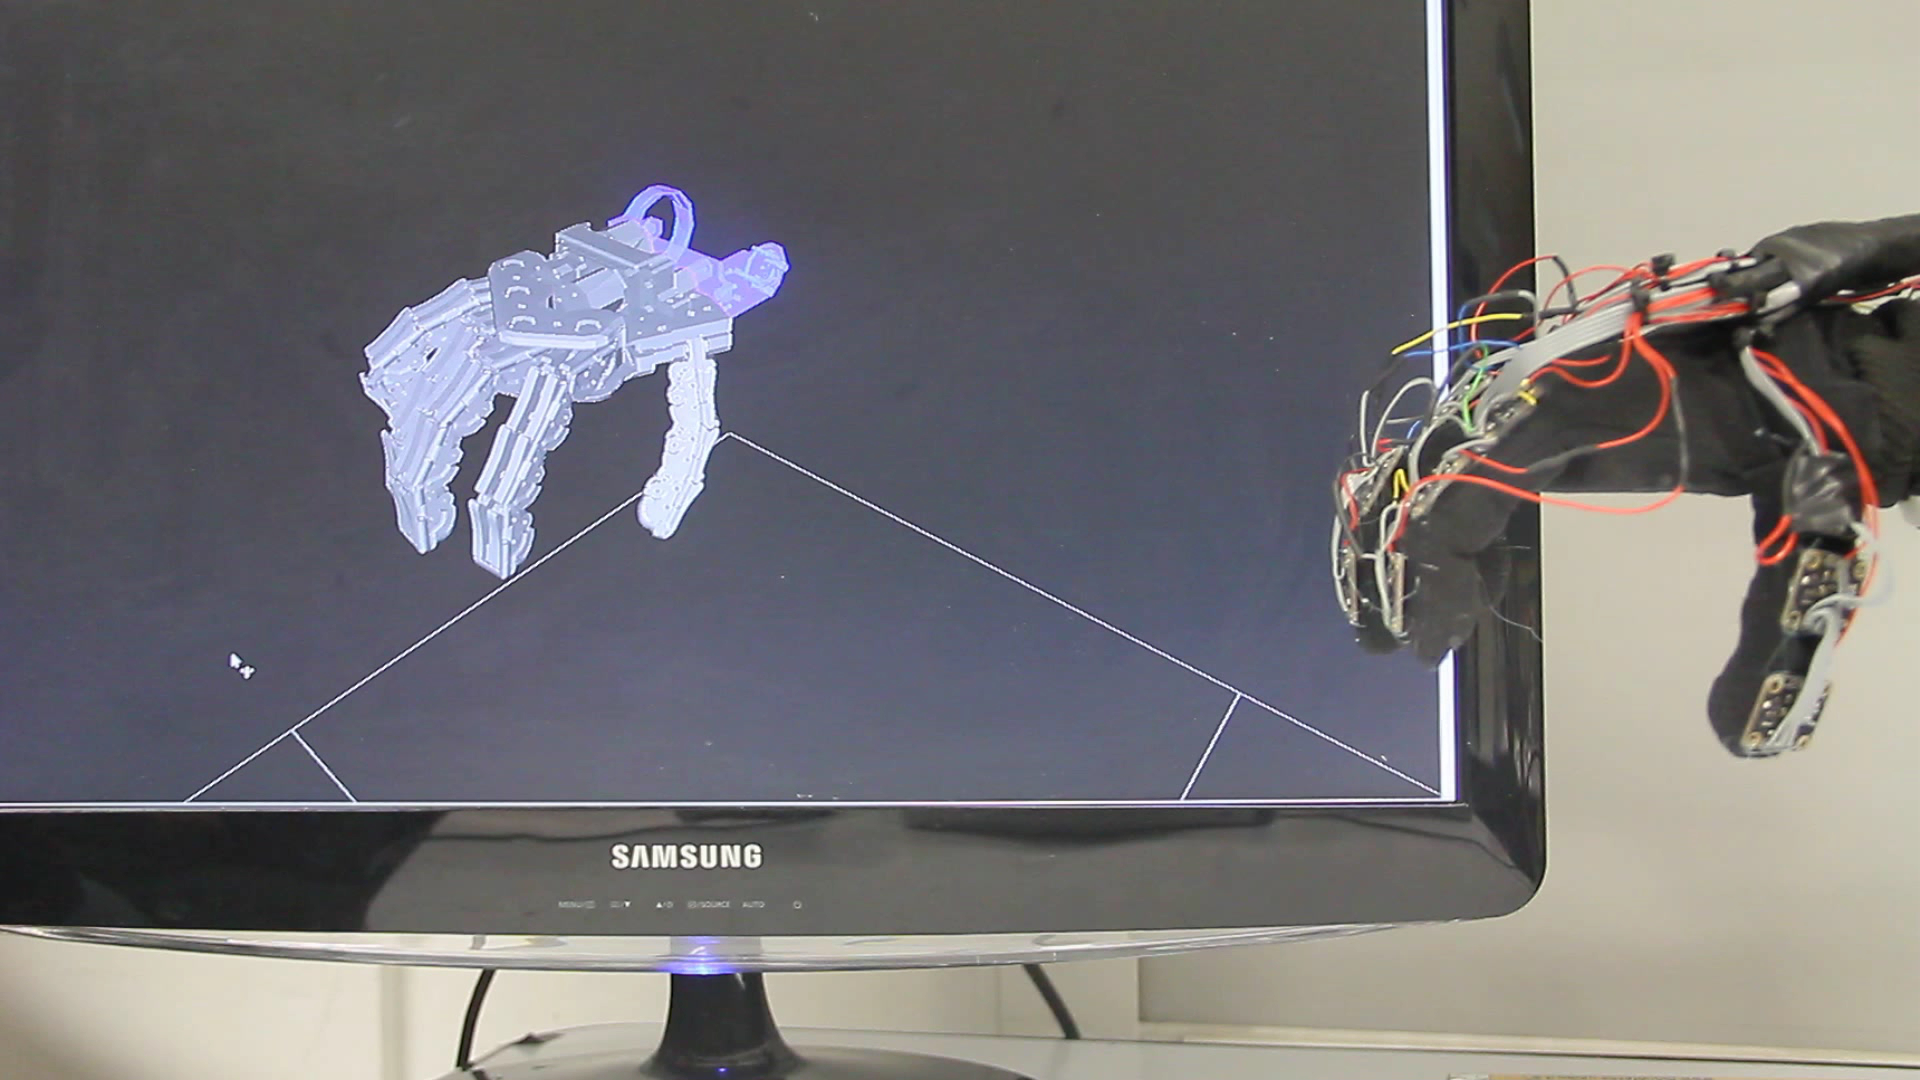
\includegraphics[width=0.33\linewidth]{Hand_Movement_2.png}
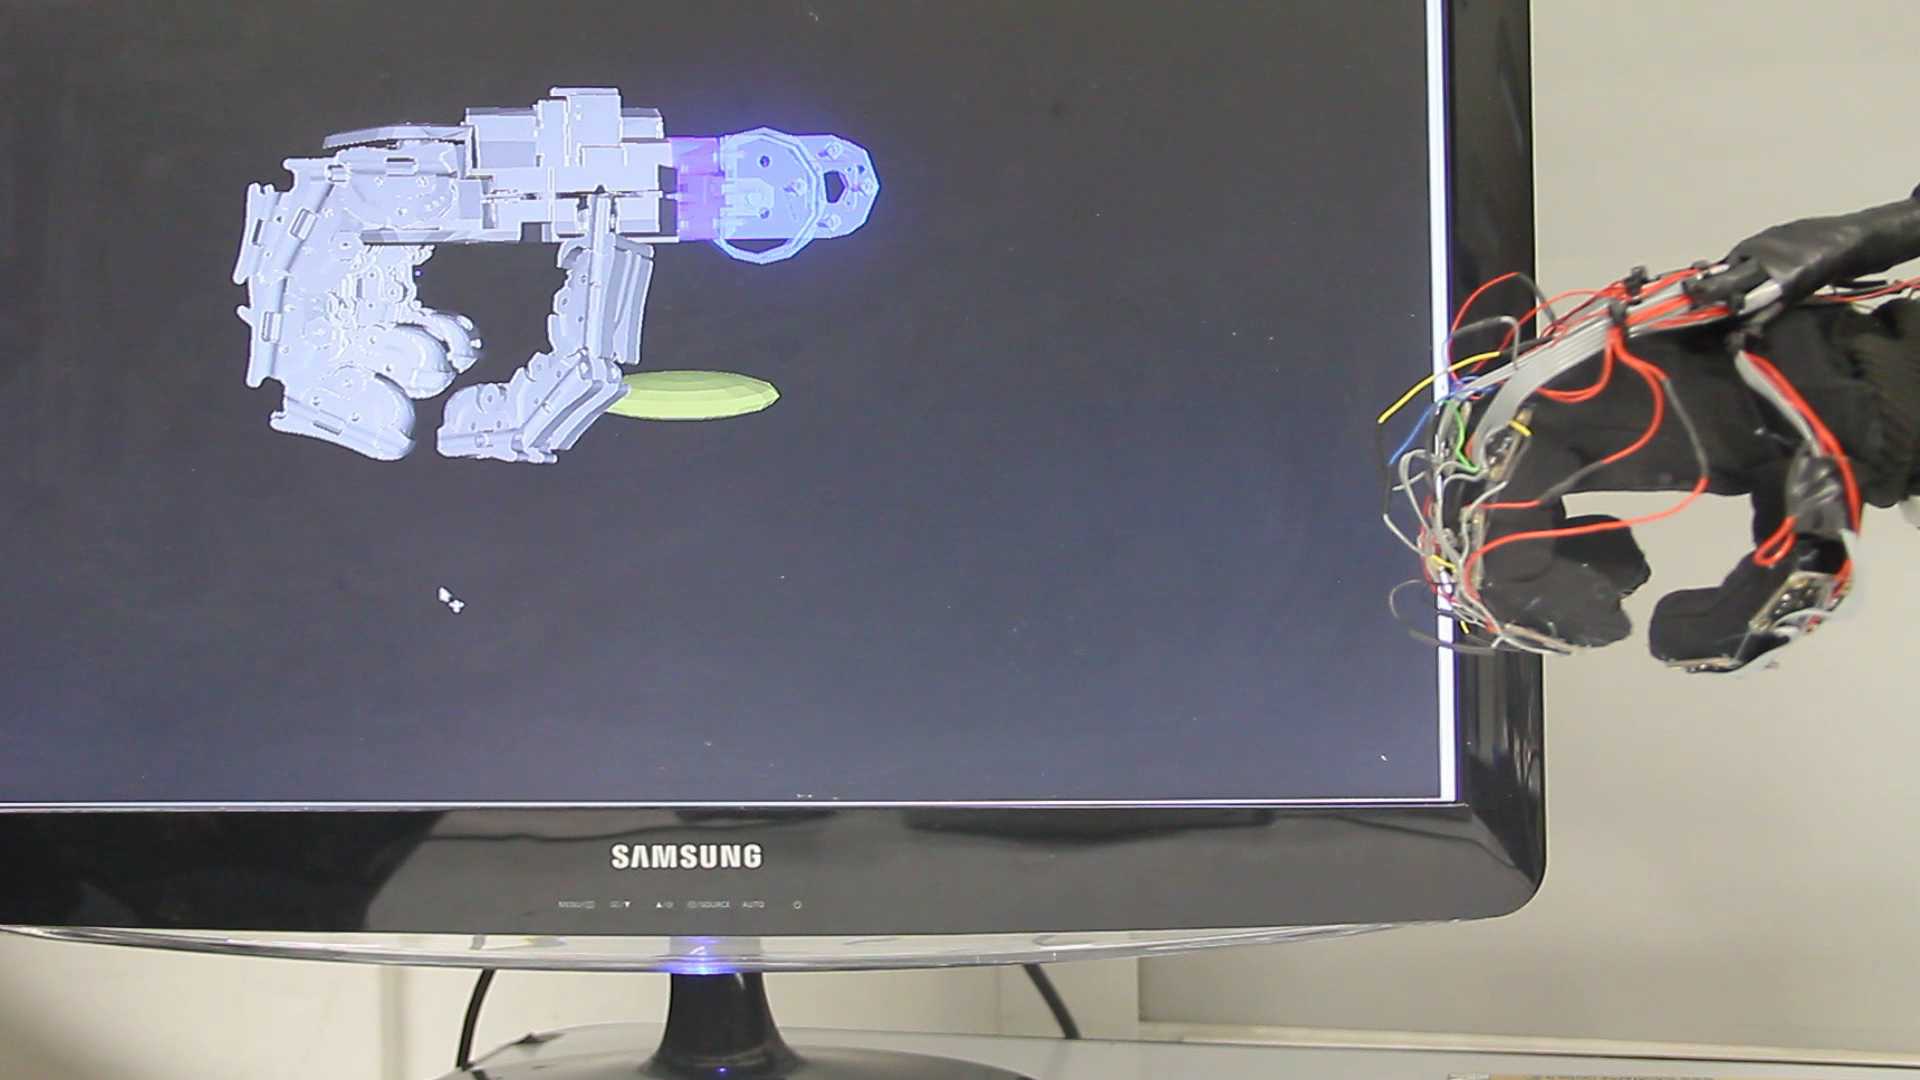
\includegraphics[width=0.33\linewidth]{Hand_Movement_3.png}
}
\caption{Hand posture reconstruction examples}
\label{fig:hand_reconstruction_1}
\end{figure}

We used a naive recognizer to test the proposed solution, and we were able to discriminate similar cups in shape but in different sizes as shown in Fig. \ref{fig:Object_1}. For more in-sight on the recognition examples, we suggest to see videos by clicking on \href{https://www.youtube.com/watch?v=d_WPQ3WmHRg}{Object 1}, \href{https://www.youtube.com/watch?v=PG38VObdl6o}{Object 2}, \href{https://www.youtube.com/watch?v=bIYhLXm90hc}{Object $3_a$}, \href{https://www.youtube.com/watch?v=IXVlBAoGKho}{Object $3_b$}, \href{https://www.youtube.com/watch?v=Efmm6-JHcxU}{Object $4_a$}, \href{https://www.youtube.com/watch?v=NZElSV_AnJ4}{Object $4_b$}, \href{https://www.youtube.com/watch?v=mDDb5oTaHzM}{Object $5_a$} and \href{https://www.youtube.com/watch?v=sLzU39zffFY}{Object $5_b$}. For more details on the implementation, refer to Sec.~\ref{sec:imuSoftHand}.

\begin{figure}
\centering
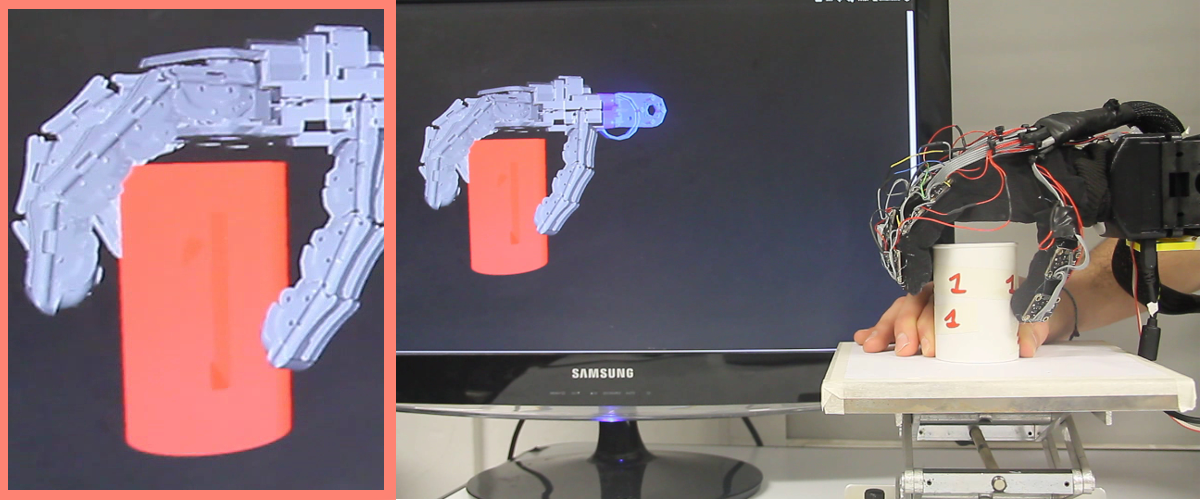
\includegraphics[width=0.8\linewidth]{Object_1.png}
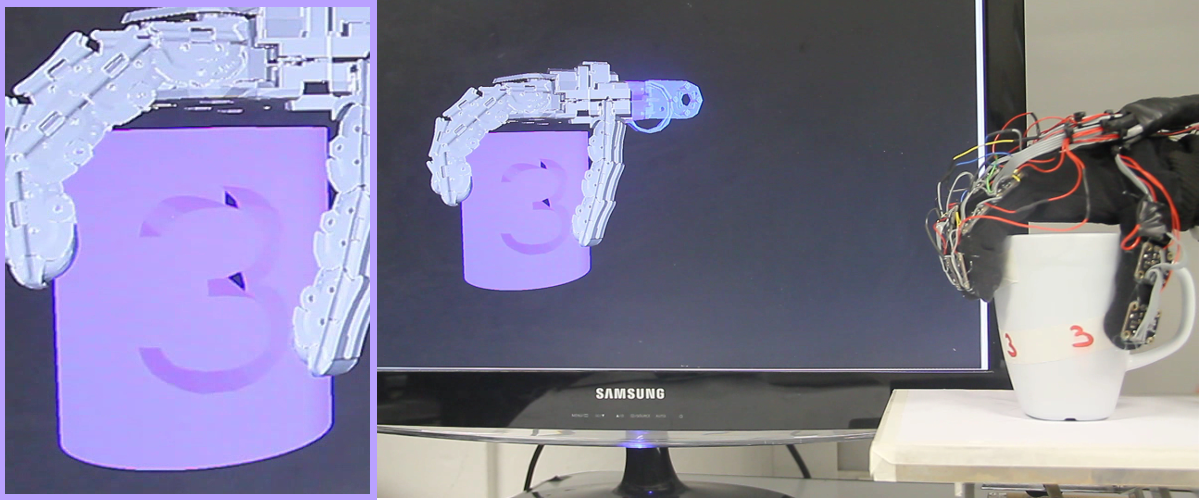
\includegraphics[width=0.8\linewidth]{Object_3.png}
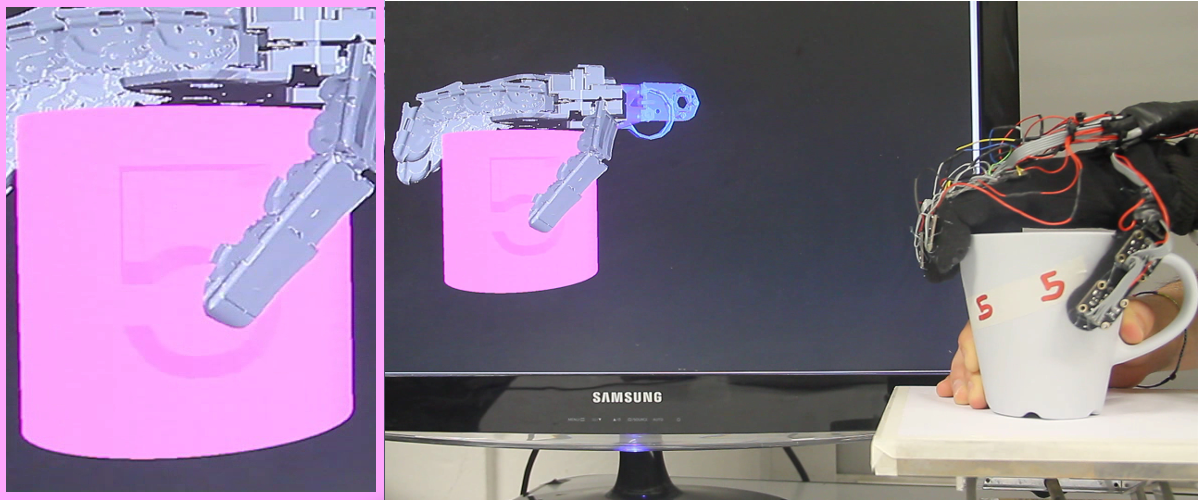
\includegraphics[width=0.8\linewidth]{Object_5.png}
\caption{Object recognition examples using the same cup of different sizes.}
\label{fig:Object_1}
\end{figure}



%%%%%%%%%%%%%%%%%%%%%%%%%%%%%%%%%%%%%%%%%%%%%%%%%%%%%%%%%%%%%%%%%%%%%%%%%%%%%%

\subsubsection{Task 3.3}

Concerning Task 3.3, we must say the the work on grasping of novel objects in WP4 progressed much faster than expected. The active gaze approach taken has thus been informed by this progress. Specifically the fact that experiments in our IJRR submission for WP4 has shown us that grasp failure is typically driven by the incompleteness of the point cloud near to suggested grasp points and along the final grasp trajectory. In addition, tests with differing numbers of views of the test object prior to grasping showed that the more views one has from an object, the greater the probability of grasping success for this object. In addition, we have used a wrist mounted depth camera for the active gaze method. We are extending the reward-based method from~\cite{nunez2013models} to the case of incomplete point clouds. We require a measure of the proportion of the total possible coverage given by the incomplete object model. To this end, we are currently investigating the use of an octree representation, called octomap~\cite{hornung13auro}, for online object modelling and sensor data fusion. The octomap of a given object allows the representation of occupied (known voxels belonging to a segmented object), free (voxels that do not belong to an object), and unknown areas of the scene, which might belong to the object if they are near known and occupied voxels. We are now implementing a method to estimate the safety of a grasp trajectory given this octomap. We are also testing different measures of the coverage of the object pertinent to a candidate grasp given the point cloud and the octomap representations.

Relevant work on grasping under incomplete information is that by Bohg and Kragic \cite{bohg:icra11}. There the approach is not active gaze to fill in information, but to use a symmetry prior to complete missing object parts. An active vision system for grasping is described in \cite{gratal:irosws10}, but in this the main goal of gaze control is to find and fixate on the object to support a visual servoing routine. There is relatively little published work that deals with active vision specifically in the service of manipulation. A more general but related problem is the use of active vision to recover the pose and complete shape of an object. Recently Krainin et al. \cite{Kra11Aut} devised a next-best-view algorithm that autonomously acquires a complete shape model of an unknown object. The next-best-view is obtained by iterating over a grid of feasible viewpoints and selecting the (relative) camera pose with the highest score adjusted for the cost of rotating the object to the new viewpoint. The work also considers the volume occupied by the robotic manipulator (the configuration of which is known), to segment the object from the robot, and to plan new grasps in order to reveal object parts that were occluded by the manipulator. This is the closest to the approach we are currently working on. Finally A recent workshop at RSS 2014 on active information gathering for grasping was notable in that none of the papers considered active vision, but instead focussed on the type of approaches we study Task 4.4.


%In year 1, we presented an algorithm for active gaze in the case where the object model is known, and the pose is uncertain. This was tested in simulation, and shown to fit human data. Relevant work on grasping under incomplete information is that by Bohg and Kragic \cite{bohg:icra11}. There the approach is not active gaze to fill in information, but to use a symmetry prior to complete missing object parts. An active vision system for grasping is described in \cite{gratal:irosws10}, but in this 
%The main goal of gaze control is to find and fixate on the object to support a visual servoing routine. A recent workshop at RSS 2014 on active information gathering for grasping was notable in that none of the papers considered active vision, but instead focussed on the type of approaches we study Task 4.4. Thus the area is underexplored.

% \subsection{Relation to the state-of-the-art}
% How are the obtained results related to the state-of-the-art?
% This part is usually discussed in the corresponding subsection. Therefore, % a global 'Relation to the state-of-the-art' is unnecessary

% To be prepared by: Jeremy Wyatt
% Active Gaze
% \input{./inputFiles/ActiveGaze.tex}
\newpage
\bibliographystyle{IEEEtran}
\bibliography{../shared_bibliography/abbreviations,./bibliography/DR31}

\newpage
\appendix
\section{Annexes}
\label{sec:annex}

% Which papers / articles are included in the report? Mention titles, authors, publication info; abstract; and a one-liner relating the publication back to the discussion on actual work performed.

\subsection{Article: Active Gathering of Frictional Properties from Objects} \label{sec:slidingPointClouds}
\begin{description}
	\item[Authors] Carlos Rosales, Arash Ajoudani, Marco Gabiccini, and Antonio Bicchi
	\item[Info] Published, see~\cite{Rosales2014Active}.
	\item[Abstract] This work proposes a representation that comprises both shape and friction, as well as the exploration strategy to gather them from an object. The representation is developed under a common probabilistic framework, particularly it uses a Gaussian Process to approximate the distribution of the friction coefficient over the surface, also represented as a Gaussian Process. The surface model is exploited to compute straight lines (geodesic flows) that guide the exploration. The exploration follows these flows by employing an impedance
controller in pursuance of safety, shape accommodation and contact enforcement, while measuring the necessary data to estimate the friction coefficient. The exploratory probes consist of an RGBD camera and an Intrinsic Tactile sensor (ITs) mounted on a robotic arm. Experimental results give evidence for the effectiveness of the algorithm in the friction coefficient gathering and enrichment of the object representation.
	\item[Relation with the deliverable] The article succesfully integrate vision with the developed controller for the sliding primitve to refine the object shape and estimate the friction coefficient (static and dynamic), and concludes Task 3.1.
	\item[Attachment] (following pages until next annex)
\end{description}
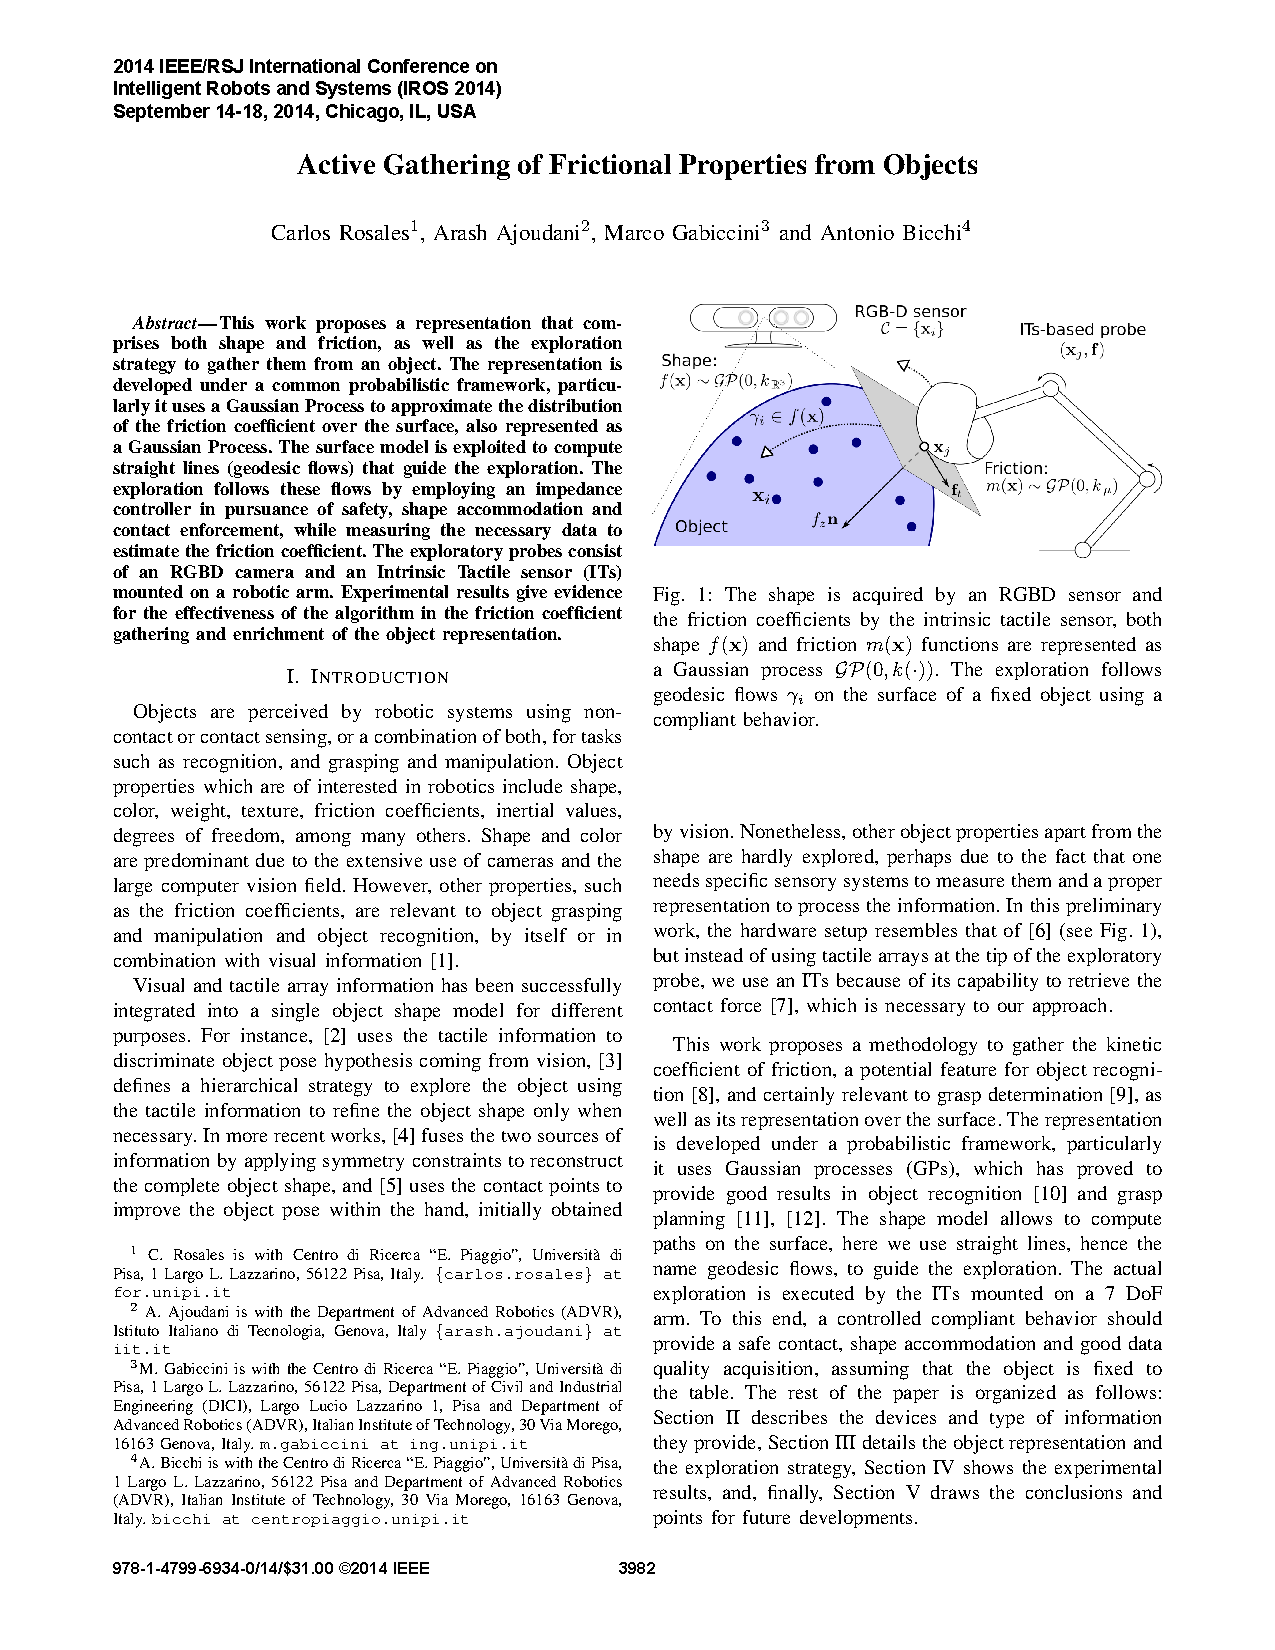
\includepdf[pages=-]{./attachedPapers/ActiveGatheringOfFrictionalPropertiesFromObjects.pdf}

\subsection{Article: Low-cost, Fast and Accurate Reconstruction of Robotic and Human Postures via IMU Measurements} \label{sec:imu2Fingers}
\begin{description}
	\item[Authors] Gaspare Santaera, Emanuele Luberto, Alessandro Serio, Marco Gabiccini, and Antonio Bicchi.
	\item[Info] Accepted for publication in Proc. of the 2015 IEEE Int. Conf. on Robotics and Automation
	\item[Abstract] In this paper, we present a method to reconstruct the configurations of kinematic trees of rigid bodies not using
measurements of relative angles (such as, e.g. rotary encoders at joints) but absolute posture sensors (such as IMUs) along with suitable filter algorithms. We argue that the relatively larger inaccuracies shown by absolute sensors can be compensated by suitable processing, such as a passive complementary filters exploiting the Mahony-Hamel formulation. The proposed method is applicable to  systems where measurements of relative angles is not feasible or convenient, or where the joint kinematics are not lower pairs: for example, human body parts or soft robotic devices. In the paper, we make explicit reference to the reconstruction of posture of the compliant, underactuated Pisa/IIT SoftHand. Quantitative comparisons with ground truth data in grasping tests are used to validate the proposed method. The resulting hardware design is mechanically robust, cheap and can be easily adapted to robotic hands with different structures, as well as to sensorizing gloves for studying human grasping strategies.
	\item[Relation with the deliverable] The proposed solution in this article is the preliminary result for the next annex.
	\item[Attachment] (following pages until next annex)
\end{description}
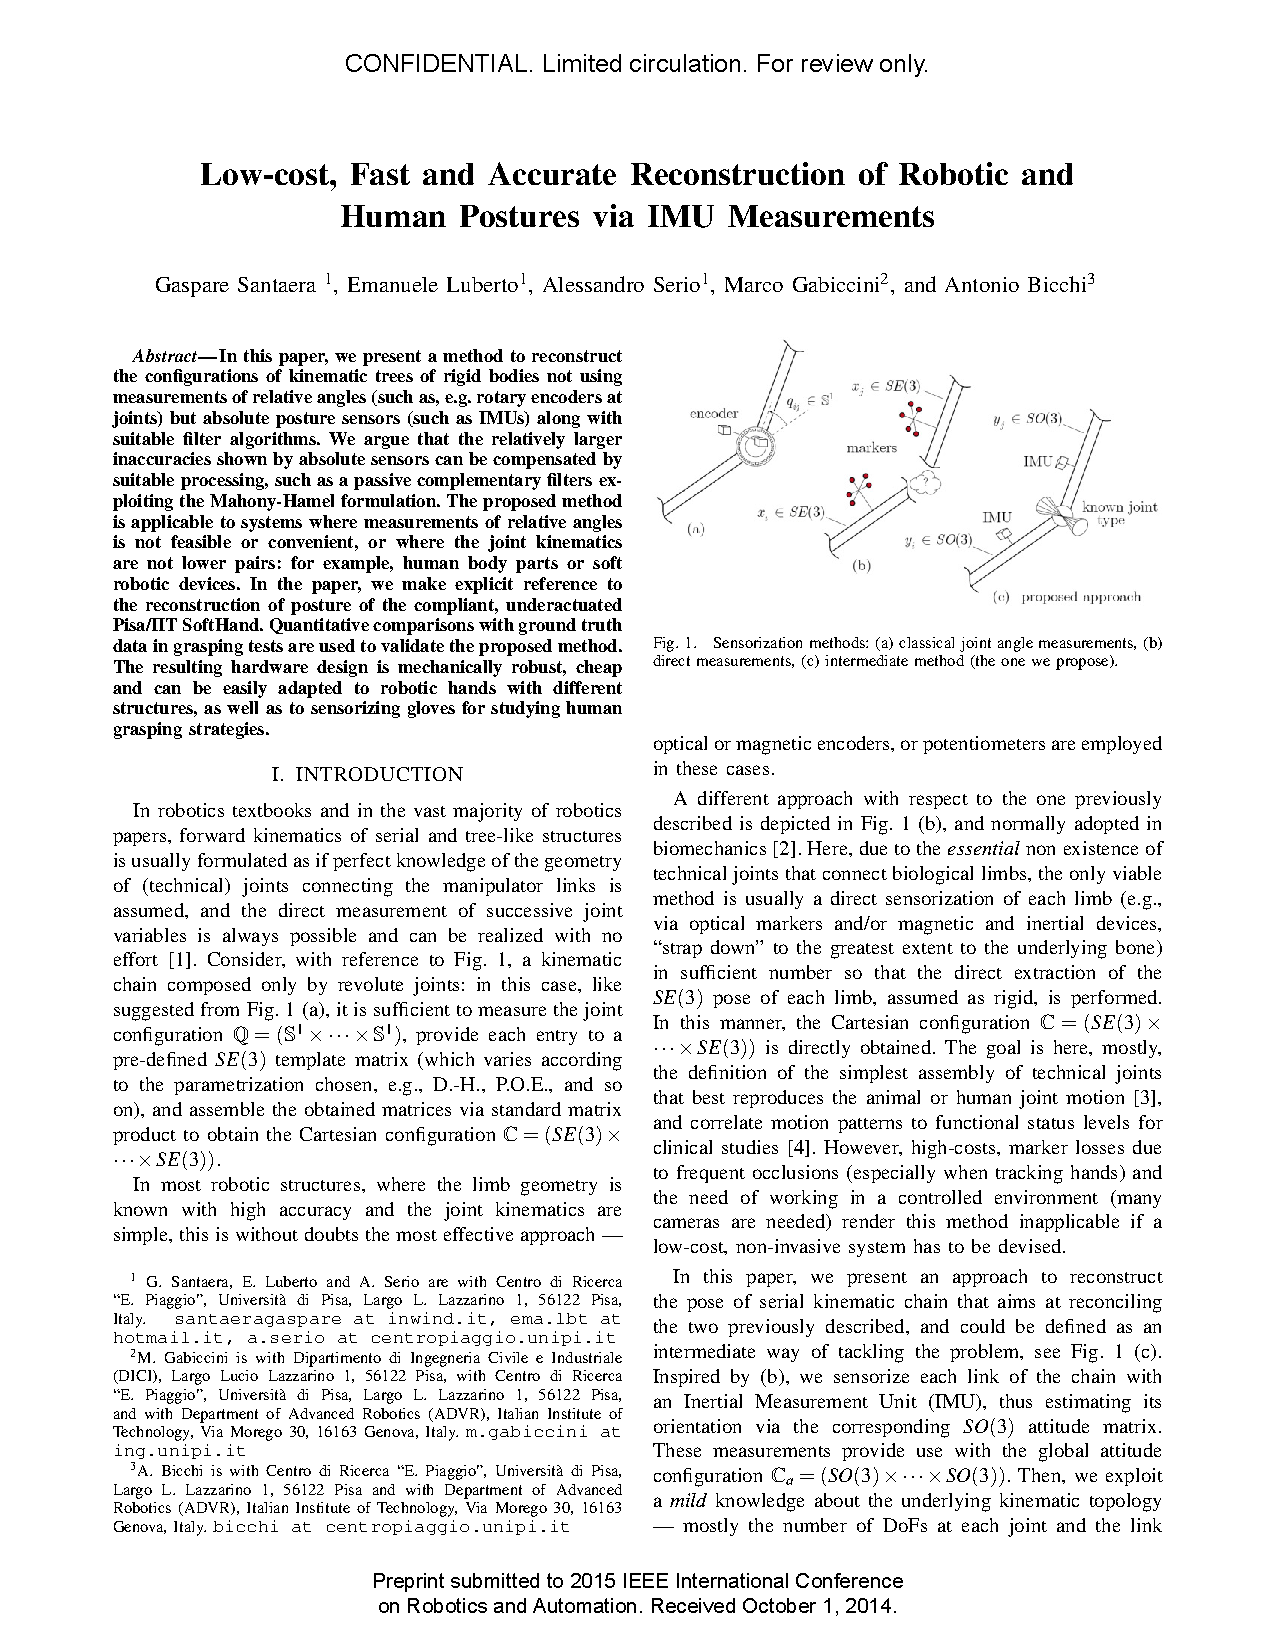
\includepdf[pages=-]{./attachedPapers/ReconstructionPosturesImuMeasurements.pdf}

\subsection{Technical report: Endowing the Pisa/IIT SoftHand with the sense of touch} \label{sec:imuSoftHand}
\begin{description}
	\item[Authors] Gaspare Santaera, Emanuele Luberto, Marco Gabiccini, and Antonio Bicchi.
	\item[Info] Internal report, in preparation for submission to a conference.
	\item[Abstract] A modified version of the Mahony-Hamel passive complementary filter is used to obtain the orientation of a frame $\{ A \}$ with respect to another frame $\{ B \}$, expressed by a rotation matrix and subject to kinematic constraints, to reconstruct a two-finger gripper. We extend that work to the five-finger Pisa/IIT SoftHand and the potential application of object recognition without vision and using a naive recognizer.
	\item[Relation with the deliverable] The proposed solution in this report aims to tackle the problem of object exploration and recognition in the case where partial or none visual information is available. This scenario is challenged in Task 3.2.
	\item[Attachment] (following pages)
\end{description}
\includepdf[pages=-]{./attachedPapers/imuSoftHand.pdf}


\end{document}
